%%
%% Author: Davidov
%% 23.04.2018
%%

\documentclass[12pt,a4paper]{book}

%underline emph
\renewcommand{\emph}[1]{\textbf{#1}}

%packages for math symbols
\usepackage{amsmath}
\usepackage{amssymb}
\usepackage{textcomp}
\usepackage{mathpartir}
\usepackage{stmaryrd}
\usepackage{mathtools}

% package for graphs
\usepackage{tikz}
\usetikzlibrary{graphs}
\usetikzlibrary{positioning}
\usetikzlibrary{automata}
\usetikzlibrary{arrows,decorations.pathmorphing,backgrounds,positioning,fit,petri}

% package for urls
\usepackage{hyperref}

%package for using
\usepackage{graphicx}

%package for proof and other theorem environments
\usepackage{amsthm}

%this package provides a pendant to "itemize" with better spacing - use compactitem
\usepackage{paralist}

%supports some nice characters with mathscr
\usepackage{mathrsfs}

%enables better support for tables
\usepackage{array}
\usepackage{multirow}

% various theorems, numbered by section
\newtheorem{theorem}{Theorem}[section]
\newtheorem{lemma}[theorem]{Lemma}
\newtheorem{proposition}[theorem]{Proposition}
\newtheorem{corollary}[theorem]{Corollary}
\newtheorem{definition}[theorem]{Definition}
\newtheorem{example}[theorem]{Example}

\newenvironment{remark}[1][Remark]{\begin{trivlist}
\item[\hskip \labelsep {\bfseries #1}]\end{trivlist}}

\newcolumntype{C}[1]{>{\parbox[c][#1][c]{0cm}{}}c<{}}

%some own commands
\newcommand{\expspace}[1]{#1-EXPSPACE/$_{\raise.17ex\hbox{$\scriptstyle\sim$}}$}
\newcommand{\exptime}[1]{#1-EXPTIME/$_{\raise.17ex\hbox{$\scriptstyle\sim$}}$}

%set of own commands
%\newcommand{\hcat}{\rotatebox{90}{$\ominus$}}
\newcommand{\hcat}{
\mathchoice{\rotatebox{90}{$\displaystyle\ominus$}}
{\rotatebox{90}{$\ominus$}}
{\rotatebox{90}{$\scriptstyle\ominus$}}
{\rotatebox{90}{$\scriptscriptstyle\ominus$}}}
\newcommand{\vcat}{
\mathchoice{\raisebox{1pt}{$\displaystyle\ominus$}}
{\raisebox{1pt}{$\ominus$}}
{\raisebox{0.5pt}{$\scriptstyle\ominus$}}
{\raisebox{0.2pt}{$\scriptscriptstyle\ominus$}}}
\newcommand{\plusinbox}{
\setlength\fboxsep{0pt}
\setlength{\fboxrule}{0.00001pt}
\text{ \framebox[8pt]{+} }
\setlength\fboxsep{3pt}
\setlength{\fboxrule}{0.4pt}
}
\newcommand{\mirroredL}{
\resizebox{0.31cm}{!}{\tiny\begin{tabular}[b]{C{0.4cm}|C{0.4cm}|}
\cline{2-2}
&\tabularnewline
\hline
\multicolumn{1}{|c|}{}&\tabularnewline
\hline
\end{tabular}}\normalsize}
%document information
\title{Comparing Deterministic Exponential Time and Space Hierarchy with Polyadic Higher Order Fixpoint Logic}

\author{David Kronenberger}

\makeatletter
\def\maketitle{%

\begin{center}
\textbf{\textsf{\Huge \@title}}\\
\vspace{2cm}
{\Large by\\
\@author\\
\vspace{2.5cm}
Dipl.-Math. Florian Bruse, Advisor\\
Prof. Dr. Martin Lange, Advisor
}\\
\vspace{2.5cm}
A thesis submitted in partial fulfillment\\
of the requirements for the\\
Degree of Master of Science\\
in Computer Science\\
\vspace{2cm}
UNIVERSITY OF KASSEL\\
Hesse, Germany\\
\vspace{1cm}
\@date
\end{center}
}

\begin{document}

\maketitle
\thispagestyle{empty}

\pagebreak

\cleardoublepage
\vspace*{30\baselineskip}
\hbox to \textwidth{\hrulefill}
\par
\hbox to \textwidth{I declare that I have developed and written the enclosed thesis entirely}
\hbox to \textwidth{by myself, and have not used sources or means without declaration in the text.}
\vspace{0.9cm}
\hbox{\textbf{Kassel, \today}}
\vspace{0.6cm}

\hbox{\ldots\ldots\ldots\ldots\ldots\ldots\ldots\ldots\ldots\ldots\ldots\ldots}~\\
\hbox{\hspace*{1cm}(\textbf{David Kronenberger})} %center name with hspace

\thispagestyle{empty}

\pagebreak

\tableofcontents
\thispagestyle{empty}
\pagebreak

\setcounter{page}{1}
\chapter{Introduction}\label{ch:introduction}

The higher order cases of PHFL and a restriction called
tail-recursive for this higher order cases we are interested to compare with the in
Section~\ref{sec:descriptiveComplexity} introduced complexity classes \exptime{$k$} and \expspace{$k$}.

\chapter{Preliminaries}
\label{ch:preliminaries}
This chapter introduces all necessary definitions to prove that PHFL$^k =$~\exptime{$k$} and
PHFL$^{k+1}_{tail} =$~\expspace{$k$}. The notions are mainly from~\cite{immerman1999descriptive},
~\cite{papadimitriou1994complexity},~\cite{otto1999bisimulation},~\cite{freireMartins2011descriptive}
and~\cite{lange2014capturing}.

We assume that the reader is already familiar with basic notions of first order logic and 
computational complexity. In the first section we define a special kind of graphs called LTS and 
define some properties on it. Also in this section we define queries with special forms of queries. 
In the next section we give some information on fixpoints that are used the section that follows. 
There is defined the logic PHFL. In Section~\ref{sec:descriptiveComplexity} we present the 
descriptive complexity and the complexity clases \exptime{$k$} and \expspace{$k$}. In the last section we define the higher-order logic and combinations with LFP and PFP.

%%
%% Author: Davidov
%% 16.05.2018
%%

\subsection{Bisimulation Invariance}\label{subsec:bisimulationInvariance}

First of all, we need the definition of \textit{labeled transition systems}. A labeled transition system is a graph
with labeled vertices and edges. Formally, it is the following.

\begin{definition}
    \label{definition:lts}
    A quintuple $\mathcal{T} = (Q, \Sigma, P, \Delta, \nu)$ is called a \emph{labeled transition system} (\emph{LTS}),
    where
    \begin{compactitem}
        \item $Q$ is a set of states,
        \item $\Sigma$ is a finite set of actions,
        \item $P$ is a finite set of propositions,
        \item $\Delta \subseteq Q \times \Sigma \times Q$ is the labeled transition relation and
        \item $\nu: Q \rightarrow 2^P$ is a function that maps each state to a set of propositions.
    \end{compactitem}
\end{definition}

For all $q_1, q_2 \in Q$ and all $a \in \Sigma$ we write $q_1 \overset{a}{\rightarrow} q_2$ for $(q_1, a, q_2) \in
\Delta$.

\begin{example}
    As mentioned above, LTS can be seen as a graph with labeled vertices and edges. One example for a LTS is
    $\mathcal{T} = (\{0, 1, 2, 3, 4\}, \{a, b\}, \{p, q\}, \Delta, \nu)$
\begin{center}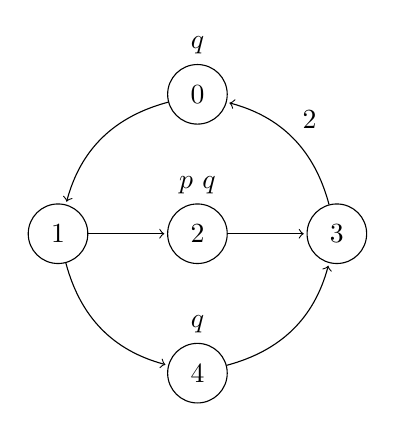
\begin{tikzpicture}[]
                  \node [place] (w1) [label=above:$q$] {0};
                  \node [place] (c1) [below=of w1,label=above:$p~q$] {2};
                  \node [place] (s) [below=of c1,label=above:$q$] {4};
                  \node [place] (e1) [left=of c1] {1}
                  edge [pre,bend left] (w1)
                  edge [post,bend right] (s)
                  edge [post] (c1);
                  \node [place] (l1) [right=of c1] {3}
                  edge [pre] (c1)
                  edge [pre,bend left] (s)
                  edge [post,bend right] node[auto, swap] {2} (w1);
\end{tikzpicture}
\end{center}
\end{example}

On this systems or rather on the states of the systems it is possible to define relations. The
following relation describes those states that have the same behaviour. For this, let be $\mathcal{T}_1 = (Q_1,
\Sigma_1, P_1, \Delta_1, \nu_1)$ and $\mathcal{T}_2 = (Q_2, \Sigma_2, P_2, \Delta_2, \nu_2)$ two LTSs.

\begin{definition}
    A \emph{bisimulation} is a binary relation $R \subseteq Q_1 \times Q_2$ that fulfills for all $(q_1, q_2) \in R$
    \begin{compactitem}
        \item $\nu_1 (q_1) = \nu_2 (q_2)$,
        \item for all $a_1 \in \Sigma_1$ and all $q_1' \in Q_1$, if $q_1 \overset{a_1}{\rightarrow} q_1' \in
        \Delta_1$, then there is a state $q_2' \in Q_2$ with $a_1 \in \Sigma_2$, $q_2
        \overset{a_1}{\rightarrow} q_2' \in \Delta_2$ and $(q_1', q_2') \in R$ and
        \item for all $a_2 \in \Sigma_2$ and all $q_2' \in Q_2$, if $q_2 \overset{a_2}{\rightarrow} q_2' \in
        \Delta_2$, then there is a state $q_1' \in Q_1$ with $a_2 \in \Sigma_1$, $q_1
        \overset{a_2}{\rightarrow} q_1' \in \Delta_1$ and $(q_1', q_2') \in R$.
    \end{compactitem}
    We call two states $q_1 \in Q_1$, $q_2 \in Q_2$ \emph{bisimilar}, noted as $(\mathcal{T}_1, q_1) \sim
    (\mathcal{T}_2, q_2)$, if there
    is a bisimulation $R$ such that $(q_1, q_2) \in R$.
\end{definition}

Furthermore, we can describe properties of LTS. \textit{Queries} are one way to describe these properties. A query
is a mapping that associates a LTS $\mathcal{T} = (Q, \Sigma, P, \Delta, \nu)$ to a subset
$M^{\mathcal{T}}$ of $Q \times \dots \times Q$. Remark, that any isomorphism $f: \mathcal{T} \simeq
\mathcal{T}'$ is also an isomorphism of $M^{\mathcal{T}}$ and $M^{{\mathcal{T}}'}$.

\begin{definition}
    \label{definition:query}
    A function $\mathcal{Q} : \mathscr{T} \rightarrow \mathscr{Q} \times \dots \times \mathscr{Q}, [\mathcal{T}]_\simeq
    \mapsto M^{\mathcal{T}}$ is called a
    \emph{$r$-adic query},
    where
    \begin{compactitem}
        \item $\mathscr{T}$ is the set of all equivalence classes of LTS relative to isomorphism,
        \item $\mathscr{Q}$ is the set of all equivalence classes of sets of states relative to isomorphism,
        \item $[\mathcal{T}]_\simeq = ([Q^\mathcal{T}]_\simeq, [\Sigma^\mathcal{T}]_\simeq, [P^\mathcal{T}]_\simeq,
        [\Delta^\mathcal{T}]_\simeq, [\nu^\mathcal{T}]_\simeq) \in \mathscr{T}$ is the equivalence class of LTS
        $\mathcal{T}$ relative to isomorphism and
        \item $M^{\mathcal{T}} \in \mathcal{P}([Q^\mathcal{T}]_\simeq \times \dots \times [Q^\mathcal{T}]_\simeq)$ is a
        set of tuples of states from $[\mathcal{T}]_\simeq$, i.e. $(q_1, \dots, q_r) \in M^{\mathcal{T}}$ with $q_1,
        \dots, q_r \in [Q^\mathcal{T}]_\simeq$.
    \end{compactitem}
\end{definition}

The queries defined in Definition~\ref{definition:query} can be categorized. Here we are interested in two of these
categories. The first category is called \textit{bisimulation invariant}. This category describes those queries that
can't distinguish bisimilar states. In~\cite{otto1999bisimulation} this property is defined over so called
\textit{Kripke structures}. A Kripke structure
is a transition system. Remark, that transition systems  have only one type of actions. This means the edges of the
graph haven't labels.

\begin{definition}
    \label{definition:bisimulationInvariant}
    Let $\mathcal{T}$, $\mathcal{T}'$ be two LTSs with $\mathcal{T} = (Q, \Sigma, P, \Delta, \nu)$
    and $\mathcal{T}' = (Q', \Sigma', P', \Delta', \nu')$. Furthermore, let be $(q_1, \dots, q_r) \in Q \times \dots
    \times Q$ and $({q_1}', \dots, {q_n}') \in Q' \times \dots \times Q'$.

    A query $\mathcal{Q}$ is called \emph{bisimulation invariant} if $(\mathcal{T}, q_i) \sim (\mathcal{T}', q_i')$
    for all $1 \leq i \leq r$ implies that $(q_1, \dots, q_r) \in \mathcal{Q}([\mathcal{T}]_\simeq)$ iff $({q_1}',
    \dots, {q_n}') \in \mathcal{Q}([\mathcal{T}']_\simeq)$.
\end{definition}

The second category of a query tells us which complexity class a query belongs to.

\begin{definition}
    \label{definition:queryBelongsToComplexityClass}
    Let $\mathcal{T}$ be a LTS with $\mathcal{T} = (Q, \Sigma, P, \Delta, \nu)$ and $(q_1, \dots, q_{r}) \in Q \times
    \dots \times Q$.

    A query $\mathcal{Q}$ belongs to complexity class $\mathcal{C}$ if there is an algorithm in $\mathcal{C}$ for
    deciding on input $(\mathcal{T}, (q_1, \dots, q_{r}))$ whether $(q_1, \dots, q_{r}) \in \mathcal{Q}
    ([\mathcal{T}]_\simeq)$.
\end{definition}

This definition leads us to the next chapter and the definitions for descriptive complexity.

%%
%% Author: Davidov
%% 16.05.2018
%%

\section{Fixpoints}\label{sec:fixpoints}

To define the polyadic higher-order fixpoint logic and the higher-order logic with least and partial fixpoints, we examine fixpoints in general in this section. The first fixpoint we consider is the least fixpoint.

\begin{definition}
   Let $F\colon A \rightarrow A$ be an operator on a finite set $A$, then $x \in A$
   is called a \emph{fixpoint} of $F$ if $F(x) = x$. Let $x$ be a fixpoint of $F$ and $\sqsubseteq$ an partial order on $A$, then $x$ is called the \emph{least
   fixpoint} of $F$, abbreviated as $\mathit{LFP}$($F$), if for all other fixpoints $y$ of $F$ the condition $x
   \sqsubseteq y$ holds. A fixpoint $x$ is called the \emph{greatest fixpoint} if $y \sqsubseteq x$ for all fixpoints $y$ of $F$.
\end{definition}

From the Knaster-Tarski Theorem~\cite{tarski1955lattice} we know that if an operator $F\colon A \rightarrow 
A$ is monotone and $A$ is a complete lattice regarding to $\sqsubseteq$ then the least and greatest fixpoints of $F$ exists. $F$ is monotone if for all $x, y
 \in A$ if $x \sqsubseteq y$ then $F(x) \sqsubseteq F(y)$ holds.

\begin{example}
    \label{example:lfp} Let $\mathcal{T} = (Q, \Sigma, P, \Delta, v)$ be an LTS and $F: Q^2 \rightarrow Q^2$ an operator on $Q^2$ defined as 
\begin{align*}
    F(X) =\, &\{(q, p) \in Q^2 \mid v(q) \neq v(p)\}\, \cup \\&
    \{(q,p) \in Q^2 \mid \text{it exists } a\in\Sigma \text{ with } q\overset{a}{\rightarrow} q' \text{ such that for all } p' \in Q \\&\text{ it holds } p\overset{a}{\rightarrow} p' \text{ implies } (q', p') \in X\}\,\cup \\&\{(q,p) \in Q^2 \mid  \text{it exists } a\in\Sigma \text{ with } p\overset{a}{\rightarrow} p' \text{ such that for all } q' \in Q \\&\text{ it holds } q\overset{a}{\rightarrow} q' \text{ implies } (q', p') \in X\}
\end{align*}   
Then $LFP(F)$ represents all those pairs of states $(q, p)$ such that $q\not\sim p$.
\end{example}

The following theorem shows a possibility to calculate the least fixpoint of a monotone operator if the operating set is a complete lattice with respect to its order.

\begin{theorem}[Kleene Fixed-Point Theorem~\cite{stoltenberghHansen1994mathematical}]
\label{theorem:kleene}
Let $F: A \rightarrow A$ be a monotone operator on $A$ and $A$ regarding to $\sqsubseteq$ a complete lattice, then it exists a finite sequence $X_0, \dots, X_m$ such that the first part $X_0$ is the smallest element in $A$ with respect to $\sqsubseteq$, the $(i+1)$-th part $X_{i+1}$ is $F(X_i)$ and $X_m = X_{m+1}$.
\end{theorem}

Next, we define the partial fixpoint. Since the
$\mathit{LFP}$ restricts the operator to be monotone, the partial fixpoint need no restriction on the operator.

\begin{definition}
\label{definition:pfp}
    Let $F\colon A \rightarrow A$ be an operator on a finite set $A$, then the \emph{partial
    fixpoint} of $F$, abbreviated as $\mathit{PFP}$($F$), is defined as follows:
    \[\mathit{PFP}(F)\coloneqq\begin{cases}
               F^{i+1}(\varnothing)=F^i(\varnothing),  & \text{if such } i \in \{0,\dots,|A|\} \text{ exists}\\
               \varnothing, & \text{otherwise,}
    \end{cases}\]
    where $F^0(\varnothing) = \varnothing$, $F^1(\varnothing) = F(\varnothing)$, $F^2(\varnothing) = F(F(\varnothing))$, and so on.
\end{definition}

Note, that for monotone $F$ holds $\mathit{PFP}(F)$ equals $\mathit{LFP}(F)$. 


\begin{example}
\label{example:pfp}
Let $F: \mathcal{P}(\{1, \dots, n\}) \rightarrow  \mathcal{P}(\{1, \dots, n\})$ be an operator on $ \mathcal{P}(\{1, \dots, n\})$ defined as
\begin{align*}
	F(X) = \{x \in \{1, \dots, n\}\mid &\; x\in X \text{ and it exists } y \in \{1, \dots, n\} \text{ such that }\\ &\;y < x \text{ and } y\not\in X \text{ or } \\&\;x\not\in X \text{ and for all } y\in \{1,\dots, n\} \text{ holds if } \\&\;y<x \text{ then } y\in X\}. 
\end{align*}
If we see $X \in \mathcal{P}(\{1,\dots, n\})$ as a binary string $b$, where a $1$ at the $i$-th position means that $i$ is in $X$, then $F(X)$ returns the set $Y$ such that the binary string $b'$ of $Y$ is $b' = b+1\mod n$. Then $PFP(F)$ returns $\varnothing$ because for every $i$ it holds $F^i(\varnothing) \neq F^{i+1}(\varnothing)$.
\end{example}

%%
%% Author: Davidov
%% 16.05.2018
%%

\section{Polyadic Higher Order Fixpoint Logic}\label{sec:polyadichigherorderfixpointlogic}

In this section, we present a logic with name Polyadic Higher Order Fixpoint Logic, abbreviated with PHFL, that was
introduced by M. Lange and E. Lozes in~\cite{lange2014capturing}. It is defined over LTS (see
Definition~\ref{definition:lts}) and extends the polyadic modal $\mu$-calculus~\cite{otto1999bisimulation} with
higher order fixpoints like M. Viswanathan and R. Viswanathan it did with monadic case of modal
$\mu$-calculus~\cite{kozen1983results} in~\cite{viswanathan2004higher}. The logic of M. Viswanathan and R
.Viswanathan with name higher order fixed point logic is a combination of propositional logic, modal operators and
a simply typed $\lambda$-calculus with fixed point operators. The higher order cases of PHFL and a restriction called
tail-recursive for this higher order cases we are interested to compare with the in
Chapter~\ref{sec:descriptiveComplexity} introduced complexity classes \exptime{$k$} and \expspace{$k$}.

\subsection{PHFL Types}\label{subsec:phflTypes}

Before defining formulas of PHFL we need to introduce the PHFL types. These definitions are guided
by~\cite{viswanathan2004higher} and~\cite{lange2014capturing}.

\begin{definition}
    \emph{PHFL types} are given by the grammar
    \[\sigma, \tau \Coloneqq \bullet \mid \sigma^v \rightarrow \tau,\]
    where $v$ is called \textit{variance}. The \emph{variances} of PHFL are defined by the grammar
    \[v \Coloneqq + \mid - \mid 0.\]
\end{definition}

All types will be interpreted as a partially ordered sets. Partial orders are relations that are reflexive, transitive
and antisymmetric. Let $\mathcal{A} = (A, \leq_A)$ and $\mathcal{B} = (B, \leq_B)$ be two partial orders. Then
$\mathcal{A} \rightarrow \mathcal{B}$ is the partial order of monotone functions ordered pointwise, i.e.
\[\mathcal{A} \rightarrow \mathcal{B} = \{f\colon A\rightarrow B \mid \text{ for all } x,y \in A.\,x\leq_A y \text{
implies }
f(x)
\leq_B f(y)\}\]
and the ordering relation is given by
\[f \leq_{\mathcal{A}\rightarrow\mathcal{B}} g\text{ iff } \text{ for all } x\in \mathcal{A}.\,f(x) \leq_{\mathcal{B}} g
(x)\].

\begin{definition}
    Let $\mathcal{T} = (Q, \Sigma, P, \Delta, v)$ be a LTS and $d \in \mathbb{N}$ the dimension of PHFL,
    then $\llbracket\tau\rrbracket_\mathcal{T}$ the
    semantics
    of type $\tau$ is defined by $\tau$ as follows:
        \[\llbracket\tau\rrbracket_\mathcal{T}=
        \begin{cases}
            (\mathcal{P}(Q^d), \subseteq),  & \text{if }\tau = \bullet\\
            ((\llbracket\sigma_1\rrbracket_\mathcal{T})^v \rightarrow \llbracket\sigma_2\rrbracket_\mathcal{T}, \leq_{
            (\llbracket\sigma_1\rrbracket_\mathcal{T})^v \rightarrow \llbracket\sigma_2\rrbracket_\mathcal{T}}), &
            \text{if }\tau = \sigma_1^v\rightarrow \sigma_2,
        \end{cases}\]
    where for any partial order $\mathcal{A} = (A, \leq_A)$, $\mathcal{A}^v = (A, \leq_A^v)$ is a partial order
    with $\leq_A^+ = \leq_A$, $\leq_A^- = \{(a, b) \mid (b, a) \in \leq_A\}$ and $\leq_A^0 = \leq_A^+ \cap \leq_A^-$.
\end{definition}

The partial orders $\llbracket\tau\rrbracket_\mathcal{T}$ for any PHFL type $\tau$ are complete lattices. That means we
have meets and joins, denoted by $\sqcap_{\llbracket\tau\rrbracket_\mathcal{T}}$ and
$\sqcup_{\llbracket\tau\rrbracket_\mathcal{T}}$, and least and greatest elements, denoted by
$\bot_{\llbracket\tau\rrbracket_\mathcal{T}}$ and $\top_{\llbracket\tau\rrbracket_\mathcal{T}}$ for any subset of
$\llbracket\tau\rrbracket_\mathcal{T}$. This ensures that the least and greatest fixpoint over all monotone PHFL types
exist~\cite{tarski1955lattice}. See Chapter~\ref{subsec:hoPlusLfp} for further information about fixpoints.

\begin{definition}
    The \emph{maximal arity} $ma(\tau)$ and the \emph{order} $ord(\tau)$ of a PHFL type $\tau$ are defined
    inductively on
    $\tau$ as follows:
\[ma(\tau)=
\begin{cases}
    1, & \text{if }\tau = \bullet\\
    max(\{n\} \cup \{ma(\tau_i)\mid1,\dots,n\}), &
    \text{if }\tau = \tau_1\rightarrow\dots\rightarrow\tau_n\rightarrow\bullet
\end{cases}\]
\[ord(\tau)=
\begin{cases}
    0, & \text{if }\tau = \bullet\\
    max(\{1 + ord(\sigma_1), ord(\sigma_2)\}), & \text{if }\tau = \sigma_1 \rightarrow \sigma_2
\end{cases}\]
\end{definition}

Next, we want to define the syntax of PHFL formulas.

\subsection{PHFL Syntax}\label{subsec:phflSyntax}

\begin{figure}
    \caption{Derivation Rules for PHFL formulas.}
    \label{figure:phfl-typing-rules}
    \begin{mathpar}
        \Gamma \vdash \top \colon \bullet \and
        \Gamma \vdash p_i \colon \bullet \and
        \inferrule{\Gamma \vdash \Phi \colon \bullet}{\Gamma \vdash \langle a \rangle_i \Phi \colon \bullet} \and
        \inferrule{\Gamma \vdash \Phi \colon \bullet}{\Gamma \vdash \{\emph{i} \leftarrow \emph{j}\}\Phi \colon
        \bullet} \and
        \inferrule{\Gamma^-\vdash\Phi\colon \bullet}{\Gamma \vdash \neg \Phi \colon \bullet} \and
        \inferrule{\Gamma\vdash\Phi \colon \tau \\ \Gamma\vdash\Psi\colon \tau}{\Gamma \vdash \Phi \vee
        \Psi \colon  \tau} \and
        \inferrule{v \in \{+, 0\} }{\Gamma, X^v \colon\tau \vdash X\colon\tau} \and
        \inferrule{\Gamma,X^v\colon\sigma\vdash \Phi\colon\tau}{\Gamma\vdash \lambda (X^v \colon \tau)
        .\Phi\colon\sigma^v\rightarrow\tau} \and
        \inferrule{\Gamma,X^+ \colon \tau \vdash \Phi\colon\tau}{\Gamma \vdash \mu (X \colon\tau). \Phi\colon\tau} \and
        \inferrule{\Gamma\vdash \Phi\colon\sigma^+ \rightarrow \tau \\ \Gamma\vdash\Psi\colon\sigma}{\Gamma \vdash
        \Phi\,\Psi \colon \tau} \and
        \inferrule{\Gamma\vdash \Phi\colon\sigma^- \rightarrow \tau \\ \Gamma^-\vdash\Psi\colon\sigma}{\Gamma \vdash
        \Phi\,\Psi \colon \tau} \and
        \inferrule{\Gamma\vdash \Phi\colon\sigma^0 \rightarrow \tau \\ \Gamma \vdash \Psi\colon\sigma \\ \Gamma^-
        \vdash\Psi\colon\sigma}{\Gamma \vdash \Phi\,\Psi \colon \tau} \and
    \end{mathpar}
\end{figure}

\begin{definition}
    Let $P$ a set of propositions, $\Sigma$ a set of actions and $\mathcal{V} = \{X_1, X_2, \dots\}$ a countable
    infinite
    set of variables, then
    \emph{$d$-adic PHFL formulas} $\Phi, \Psi,\dots$ are defined by the grammar
    \begin{align*}
        \Phi,\Psi\Coloneqq&\top \mid p_i \mid \Phi \vee \Psi \mid \neg \Phi \mid \langle a \rangle_i \Phi \mid
        \{\emph{j}\,\} \Phi \mid X \mid \lambda (X^v\colon\tau).\Phi \mid \Phi\,\Psi\mid  \mu (X\colon\tau).\Phi
    \end{align*}
    where
    \begin{compactitem}
        \item $\emph{j} = (e(1), \dots, e(d))$ and $e: \{1, \dots, d\} \rightarrow \{1, \dots, d\}$,
        \item $i \in \{1, \dots, d\}$
        \item $v$ is a variance,
        \item $\tau$ is a type,
        \item $p \in P$,
        \item $a \in \Sigma$ and
        \item $X \in \mathcal{V}$.
    \end{compactitem}
\end{definition}

For convenience, we use some other further standard notations like $\Phi \wedge \Psi$, $[a]_i\Phi$, $\nu
X \colon \tau.\Phi$ or $\Phi \Leftrightarrow \Psi$. Note, that this logic is defined over LTS. The formulas are
often interpreted as a game played by two players moving pebbles along the transitions of an LTS. The two players
are called Prover and Refuter. So, $p_i$ can be interpreted as, the position of the $i$-th pebble fulfills
property $p$. $\langle a \rangle_i \Phi$ means, Prover has to move the $i$-th pebble along an $a$-transition and
check if there holds $\Phi$. With the formula $\{\emph{j}\,\} \Phi$ is mentioned, that all pebbles
are moved from Prover to the positions described by tuple $\emph{j}$ and after this $\Phi$ have to
be fulfilled. The player who has to move the pebbles changes on negations. $\lambda (X^v\colon\tau).\Phi$ is
interpreted as a function that expects arguments of $(\llbracket\tau\rrbracket_\mathcal{T})^v$. We see, that the
formulas also have types. For this, we have ensure that a formula is well-typed.

\begin{definition}
    Let $X_1, \dots, X_n$ variables, $\Phi$ a PHFL formula, $v_1, \dots, v_n$ variances and $\tau, \tau_1, \dots,
    \tau_n$ types, then $\Gamma = X_1^{v_1}\colon \tau_1, \dots X_n^{v_n} \colon \tau_n$ is
    called a \emph{type environment} and $\Gamma \vdash \Phi\colon\tau$
    is called a \emph{type judgement}. Let $\Gamma^- = X_1^{v_1^-}\colon \tau_1, \dots
    X_n^{v_n^-} \colon \tau_n$ be a type environment then $\Gamma^- = X_1^{v_1^-}\colon \tau_1, \dots
    X_n^{v_n^-} \colon \tau_n$, where $-^- = +$, $+^- = -$ and $0^- = 0$.
\end{definition}

A type judgment is called \textit{derivable} if it generates a derivation tree according to the rules of
Figure~\ref{figure:phfl-typing-rules}. This type system ensures that we do not create senseless formulas like
$\langle a \rangle_i p_j p_k$. Furthermore, it can order formulas with semantics and guarantees so monotonicity. A
formula $\Phi$ is called \textit{well-typed} if the type judgement $\emptyset \vdash \Phi:\tau$ is derivable for some
type $\tau$. Note, that we are here only interested in well-typed formulas. For those formulas where also the variable
types are obvious, we omit the type on the variables.

\subsection{PHFL Semantics}\label{subsec:phflSemantics}

\begin{figure}
    \caption{Semantics of PHFL formulas.}
    \label{figure:phfl-semantics}
    \begin{align*}
        \llbracket \Gamma \vdash \top \colon \bullet \rrbracket^\eta_\mathcal{T} =\,& Q^d\\
        \llbracket \Gamma \vdash p_i \colon \bullet \rrbracket^\eta_\mathcal{T} =\,& \{(q_1, \dots, q_d) \in Q^d \mid p \in v
        (q_i)\}\\
        \llbracket \Gamma \vdash \langle a \rangle_i \Phi \colon \bullet \rrbracket^\eta_\mathcal{T} =\,& \{(q_1,
        \dots, q_d) \in Q^d \mid \text{ it exists } \\& ({q'}_1, \dots, {q'}_d) \in \llbracket \Gamma \vdash \Phi \colon
\bullet \rrbracket^\eta_\mathcal{T} \text{ such that } \\&q_i \overset{a}{\rightarrow} {q'}_i \text{ and for all } j
        \neq
        i \text{ holds } q_j = {q'}_j\}\\
        \llbracket \Gamma \vdash \Phi \vee \Psi \colon \tau \rrbracket^\eta_\mathcal{T} =\,& \llbracket \Gamma \vdash \Phi
        \colon \tau \rrbracket ^\eta_\mathcal{T} \sqcup_\tau \llbracket \Gamma \vdash \Psi \colon \tau \rrbracket ^\eta_\mathcal{T}\\
        \llbracket \Gamma \vdash \neg \Phi \colon \bullet \rrbracket^\eta_\mathcal{T} =\,& Q^d \setminus \llbracket
        \Gamma^- \vdash \Phi
        \colon \bullet \rrbracket ^\eta_\mathcal{T}\\
        \llbracket \Gamma \vdash \{\emph{j}\} \Phi \colon \bullet \rrbracket^\eta_\mathcal{T} =\,&
        \{\{(q_1, \dots, q_d) \in Q^d \mid \\ &(q_{j_1}, \dots, q_{j_d}) \in \llbracket \Gamma \vdash \Phi
        \colon \bullet
        \rrbracket ^\eta_\mathcal{T}\}\\
        \llbracket \Gamma, X \colon \tau \vdash X \colon \tau \rrbracket^\eta_\mathcal{T} =\,& \eta(X)\\
        \llbracket \Gamma \vdash \mu (X \colon \tau).\,\Phi \colon \tau \rrbracket^\eta_\mathcal{T} =\,&
        \bigsqcap\,_{\llbracket\tau\rrbracket_\mathcal{T}} \{\mathcal{X} \in \llbracket \tau \rrbracket_\mathcal{T}
        \mid \\
        &\llbracket \Gamma, X^+ \colon \tau \vdash \Phi \colon \tau \rrbracket^{\eta[X \mapsto \mathcal{X}]}_\mathcal{T}
        \leq_{\llbracket \tau \rrbracket_\mathcal{T}} \mathcal{X}\}\\
        %\llbracket         \Gamma
 %       \vdash
  %      \lambda X^+ \colon \tau.\Phi \colon \tau \rrbracket ^\eta_\mathcal{T}\\
        \llbracket \Gamma \vdash \lambda (X^v \colon \sigma).\,\Phi \colon \sigma^v \rightarrow \tau \rrbracket
        ^\eta_\mathcal{T} =\,& F \in \llbracket \sigma^v \rightarrow \tau \rrbracket_\mathcal{T} \text{ such that for
        all }
        \mathcal{X} \in \llbracket \sigma \rrbracket_\mathcal{T}.\, \\
        &F(\mathcal{X}) = \llbracket \Gamma, X^v \colon \sigma \vdash \Phi \colon \tau \rrbracket^{\eta[X \mapsto
        \mathcal{X}]}_\mathcal{T}\\
        \llbracket \Gamma \vdash \Phi\,\Psi \colon \tau \rrbracket^\eta_\mathcal{T} =\,& \llbracket \Gamma \vdash \Phi
        \colon \sigma
        ^v \rightarrow \tau \rrbracket ^\eta_\mathcal{T}(\llbracket \Gamma \vdash \Psi \colon \sigma \rrbracket ^\eta_\mathcal{T})
    \end{align*}
\end{figure}

To define the semantics of PHFL formulas we need a mapping $\eta$ that associates to each variable an element of its
type semantics, i.e. $\eta(X) \in \llbracket\tau\rrbracket_\mathcal{T}$ for $X$ of type $\tau$. Let $\Phi$ be a
well-typed formula of type $\tau$, $\mathcal{T}$ a LTS and $\eta$ a variable mapping, then the semantics
$\llbracket\Gamma \vdash \Phi\colon \tau \rrbracket^\eta_\mathcal{T}$ are defined inductively on $\Phi$ which maps to
an element of $\llbracket\tau\rrbracket_\mathcal{T}$ as explained in Figure~\ref{figure:phfl-semantics}.
Note, that $\eta[X \mapsto \mathcal{X}]$ is a mapping $\eta'$ that is equal to $\eta$ but $\eta'(X) = \mathcal{X}$.

In this thesis we are interested in PHFL formulas that have a specific order. For this, a formula $\Phi$ has order $k$
if $k = max(\{ord(\tau)\mid \Psi \colon \tau$ \textit{is a subformula of} $\Phi\})$. The set of formulas that have
order at most $k$ is denoted by PHFL$^k$.

\begin{example}{\cite{lange2014capturing}}
    \label{example:phfl_order_2}
    The following $2$-adic PHFL$^1$ formula $\Phi$ describes trace equivalence of two states in a LTS i.e. it denotes
    those pairs $(q_1, q_2)$ for which $q_1$ has the same traces as $q_2$ and vice versa.
    \begin{align*}
        \Phi = &(\mu (F \colon \bullet^0 \rightarrow (\bullet^0 \rightarrow \bullet)).\,
        \lambda (X \colon \bullet).\, \lambda (Y \colon \bullet).\, \\&X \Leftrightarrow Y \wedge
        \underset{a \in \Sigma}{\bigwedge} F \langle a \rangle_1 X \langle a \rangle_2 Y)\top \top
    \end{align*}
\end{example}

\begin{example}{\cite{lange2014capturing}}
    \label{example:phfl_order_0}
    The following $2$-adic PHFL$^0$ formula $\Phi_\sim$ describes bisimilarity i.e. it denotes
    those pairs $(q_1, q_2)$ such that $q_1 \sim q_2$ and vice versa.
    \begin{align*}
        \Phi_\sim = \nu (X \colon \bullet).\,
        \underset{a \in \Sigma}{\bigwedge} [a]_1 \langle a \rangle_2 X \wedge [a]_2 \langle a \rangle_1 X \wedge
        \underset{p \in P}{\bigwedge} p_1 \Leftrightarrow p_2
    \end{align*}
\end{example}

Before looking at the tail-recursive fragment see the following definition of $r$-adic queries that are associated to a
closed $d$-adic formula $\Phi$.

\begin{definition}
    Given a dimension $d$ of PHFL, a type judgment $\Gamma$, a variable assignment $\eta$ and a closed $d$-adic PHFL
    formula $\Phi$ we call a $r$-adic query $\mathcal{Q}^r_\Phi$ associated to $\Phi$ if there is for all LTS
    $\mathcal{T}$ and all $(q_1, \dots, q_r) \in {\mathcal{Q}^r_\Phi}^\mathcal{T}$ a $(s_1, \dots, s_d) \in
    \llbracket \Gamma \vdash \Phi \colon \bullet \rrbracket^\eta_\mathcal{T}$ such that $q_i = s_i$ for all $i \in
    \{1, \dots, min(\{r, d\})\}$.
\end{definition}

For example $\mathcal{Q}^2_{\Phi_\sim}$ is the same query as in Example~\ref{example:query_bisimulation}, where
$\Phi_\sim$ is the formula from Example~\ref{example:phfl_order_0}.

\subsection{Tail-Recursive PHFL}\label{subsec:tail-recursivePhfl}


\begin{figure}
    \caption{Derivation Rules for PHFL formulas that shall be tail-recursive.}
    \label{figure:phfl-tail-recursive}
    \begin{mathpar}
        \bar{Y} \vdash tail(p_i, \bar{X}) \and
        \inferrule{X \in \bar{X} \cup \bar{Y}}{\bar{Y} \vdash tail(X, \bar{X})} \and
        \inferrule{\bar{Y} \vdash tail(\Phi, \emptyset)}{\bar{Y} \vdash tail(\neg \Phi, \bar{X})} \and
        \inferrule{\bar{Y} \vdash tail(\Phi, \bar{X})}{\bar{Y} \vdash tail(\{\emph{j}\} \Phi,
        \bar{X})} \and
        \inferrule{\bar{Y} \vdash tail(\Phi, \bar{X}) \\ \bar{Y} \vdash tail(\Psi, \bar{X})}{\bar{Y} \vdash tail
        (\Phi \vee \Psi, \bar{X})} \and
        \inferrule{\bar{Y} \vdash tail(\Phi, \bar{X})}{\bar{Y} \vdash tail(\langle a \rangle_i \Phi, \bar{X})} \and
        \inferrule{\bar{Y} \vdash tail(\Phi, \emptyset)}{\bar{Y} \vdash tail([a]_i \Phi, \bar{X})} \and
        \inferrule{\bar{Y} \cup \{Z\} \vdash tail(\Phi, \bar{X})}{\bar{Y} \vdash tail(\lambda Z^v \colon \tau . \Phi,
        \bar{X})} \and
        \inferrule{\bar{Y} \vdash tail(\Phi, \emptyset) \\ \bar{Y} \vdash tail(\Psi, \bar{X})}{\bar{Y} \vdash tail
        (\Phi \wedge \Psi, \bar{X})} \and
        \inferrule{\bar{Y} \vdash tail(\Phi, \bar{X}) \\ \bar{Y} \vdash tail(\Psi, \emptyset)}{\bar{Y} \vdash tail
        (\Phi\,\Psi, \bar{X})} \and
        \inferrule{\bar{Y} \vdash tail(\Phi, \bar{X} \cup \{Z\})}{\bar{Y} \vdash tail(\mu Z \colon \tau . \Phi,
        \bar{X})} \and
        \inferrule{\bar{Y} \vdash tail(\Phi, \bar{X} \cup \{Z\})}{\bar{Y} \vdash tail(\nu Z \colon \tau . \Phi,
        \bar{X})}
    \end{mathpar}
\end{figure}

Next, we want to define a fragment of PHFL formulas. This fragment is called tail-recursive and ensures that
some combinations of subformulas do not appear in an PHFL formula. For this, let the logical connective
$\wedge$, the modality operators $[a]_i$ and the greatest fixpoint operator $\nu$ be further primitives of PHFL formula
syntax. Intuitively, tail-recursive PHFL formulas are PHFL formulas where all fixpoint variables do not occur freely
under the operators $\neg$ and $[a]_i$ nor in $\Psi$ of formulas of the type $\Phi\,\Psi$ or $\Psi \wedge \Phi$.

\begin{definition}
    A closed PHFL formula $\Phi$ is called \emph{tail-recursive} if $\emptyset \vdash tail(\Phi, \emptyset)$ is
    derivable via the rules in Figure~\ref{figure:phfl-tail-recursive}.
\end{definition}

The set of all tail-recursive PHFL formulas that have order at most $k$ is denoted by PHFL$^k_{tail}$.

\begin{example}{\cite{lange2014capturing}}
    Looking at Figure~\ref{figure:phfl-tail-recursive}, we can see, that $\Phi_1 = \mu X.[a]_1 X$ is not tail
    recursive, because $X$ occurs under $[a]_1$. Also $\Phi_2 = \mu F .\lambda X. (F X) \wedge (F(F X))$
    is not tail-recursive because $F$ occurs on the left side of the logical operator $\wedge$. The second reason why
    $\Phi_2$ is not tail-recursive is because $F$ also occurs in $F X$ of subformula $F (F X)$. An example of a
    formula that is tail-recursive is given by:
    \[\nu F. \lambda X. (F \langle a \rangle_1 X) \vee (X \wedge \langle a \rangle_2 (F X))\bot\]
\end{example}

%%
%% Author: Davidov
%% 27.04.2018
%%

\subsection{Descriptive Complexity}\label{subsec:descriptiveComplexity}

One way to describe complexity classes is with the help of \textit{Turing Machines}~\cite{hopcroft1994einfuehrung}.

\begin{definition}
    The seven-tuple $M = (Q, \Sigma, \Gamma, \delta, q_0, \Box, F, R)$ is called a \emph{Deterministic Turing Machine}
    ($\mathit{DTM}$),
    where
    \begin{compactitem}
        \item $Q$ is the finite set of states,
        \item $\Sigma$ is the input alphabet,
        \item $\Gamma$ is the working alphabet with $\Sigma \subset \Gamma$,
        \item $\delta : (Q \setminus (F \cup R)) \times \Gamma \rightarrow Q \times \Gamma \times \{L, R, N\}$ is the
        transition function,
        \item $q_0 \in Q$ is the initial state,
        \item $\Box \in \Gamma \setminus \Sigma$ is the blank symbol,
        \item $F \subseteq Q$ is the set of accepting states and
        \item $R \subseteq Q$ is the set of rejecting states.
    \end{compactitem}
\end{definition}

\begin{example}
    \label{example:dtm}
    As an example for a $\mathit{DTM}$ let
    \[M = (\{q_0, q_f, q_r\}, \{a, b\}, \{a, b, \Box\}, \delta, q_0, \Box, \{q_f\}, \{q_r\})\]
    where $\delta(q_0, a)= (q_0, \Box, R)$, $\delta(q_0, b) = (q_r, b, L)$, $\delta(q_0, \Box) = (q_f, \Box, N)$.
    $M$ is a $\mathit{DTM}$ that accepts all input words that contain no symbol $b$, i.e. $L(M) = \{a\}^*$.
\end{example}

Configurations are snapshots of $\mathit{DTM}$s working on an input word. This includes the working tape, the current
state and the current position of the reading head. Formally, $C_i^M(w) = \Gamma^m \cdot Q \cdot (\Gamma^n | \Box)$
is called the $i$-th configuration of a $\mathit{DTM}$ $M = (Q, \Sigma, \Gamma, \delta, q_0, \Box, F)$ for input word
$w \in \Sigma^*$, where $m \geq 0$ and $n \geq 1$. In addition, $\Gamma^m$ represents the word of all symbols left
from the reading head position to the last symbol that is unequal to the blank symbol. $\Gamma^n$ represents the word
of all symbols right of the reading head position to the last symbol that is unequal to the blank symbol. If there
are no symbols unequal to the blank symbol right of the reading head position, the blank symbol $\Box$ of $M$ is used
instead of $\Gamma^n$.

\begin{definition}
    Let $C_i^M(w) = \gamma_1^i\dots\gamma_{m_i}^i{q_i}{\gamma_1^i}'\dots{\gamma_{n_i}^i}'$, $C_j^M(w) =
    \gamma_1^j\dots\gamma_{m_j}^j{q_j}{\gamma_1^j}'\dots{\gamma_{n_j}^j}'$ two configurations of a $\mathit{DTM}$ $M = (Q, \Sigma,
    \Gamma,
    \delta, q_0, \Box, F)$ for input word $w \in \Sigma^*$ with $i \neq j$. $C_j^M(w)$ is the next configuration
    of $C_i^M(w)$ written as $C_i^M(w) \rightarrow_M C_j^M(w)$ iff $j = i + 1$ and
    \begin{compactitem}
        \item $m_j = m_i - 1$, $\gamma_1^j = \gamma_1^i, \dots \gamma_{m_j}^j = \gamma_{m_j}^i$, $n_j = n_i + 1$,
        ${\gamma_1^j}' = \gamma_{m_i}^i, {\gamma_2^j}' = a, {\gamma_3^j}' = {\gamma_2^i}' \dots {\gamma_{n_j}^j}' =
        {\gamma_{{n_j}- 1}^i}'$ and $\delta(q_i, {\gamma_1^i}') = (q_j, a, L)$ or
        \item $m_j = m_i + 1$, $\gamma_1^j = \gamma_1^i, \dots \gamma_{m_j-1}^j = \gamma_{m_j-1}^i, \gamma_{m_j}^j
        = a$, $n_j = n_i - 1$, ${\gamma_1^j}' = {\gamma_2^i}', \dots {\gamma_{n_j}^j}' = {\gamma_{{n_j}+1}^i}'$ and
$\delta (q_i, {\gamma_1^i}') = (q_j, a, R)$ or
        \item $m_j = m_i$, $\gamma_1^j = \gamma_1^i, \dots \gamma_{m_j}^j = \gamma_{m_j}^i$, $n_j = n_i$, ${\gamma_1^j}'
= a, {\gamma_2^j}' = {\gamma_2^i}' \dots {\gamma_{n_j}^j}' = {\gamma_{n_j}^i}'$ and $\delta
        (q_i, {\gamma_1^i}') = (q_j, a, N)$.
    \end{compactitem}
    $C_i^M(w) \rightarrow_M C_j^M(w)$ is called a \emph{transition} of $M$ on $w$.
\end{definition}

The start configuration for an input word $w$ of a $\mathit{DTM}$ $M$ is $C_0^M(w) = q_0w$, where $q_0$ is the
initial state of $M$. A run of $\mathit{DTM}$ $M$ on input word $w$ is a sequence of transitions, $C_0^M(w)
\rightarrow_M C_1^M(w) \rightarrow_M C_2^M(w) \rightarrow_M \dots \rightarrow_M C_n^M(w)$, where $C_n^M(w)$ includes
either an accepting or rejecting state. A run is accepting if there is a $n \in \mathcal{N}$ such that $C_0^M(w)
\rightarrow_M C_1^M(w) \rightarrow_M \dots \rightarrow_M C_n^M(w)$ and $C_n^M(w)$ contains an accepting state of $M$.

\begin{example}
    \label{example:run_of_dtm}
    Let $M$ be the $\mathit{DTM}$ from Example~\ref{example:dtm} and $w_1 = aaba$, $w_2 = aaaa$ two input words. The
    run of $M$ on $w_1$ is
    \[C_0^M(w_1) = q_0aaba \rightarrow_M q_0aba \rightarrow_M q_0ba \rightarrow_M q_r\Box ba = C_3^M(w_1)\]
    and the run of $M$ on $w_2$ is
    \[C_0^M(w_2) = q_0aaaa \rightarrow_M q_0aaa \rightarrow_M q_0aa \rightarrow_M q_0a \rightarrow_M q_0\Box
    \rightarrow_M q_f\Box = C_5^M(w_2)\]
\end{example}

Remark, that it is possible to define $\mathit{DTM}$s that does not accept or reject any input word. For example, let
$M = (\{q_0\}, \{a\}, \{a, \Box\}, \delta, \emptyset, \emptyset)$, where $\delta(q_0, x) = (q_0, x, N)$ with $x \in
\{a, \Box\}$. $M$ is a DTM where any calculation of an input word $w$ looks as follows $q_0w \rightarrow_M q_0w
\rightarrow_M \dots$. It never reaches an accepting or rejecting state. In this thesis, we are only interested in
$\mathit{DTM}$s that reaches an accepting or rejecting state in finite time on any input word.

Known from computational complexity theory~\cite{papadimitriou1994complexity}, the time and space classes
can be defined by functions. These functions have as input a natural number that represents the length of an input
word of a $\mathit{DTM}$. In case of time classes the output of the functions depends on the number of configuration
steps. In case of space classes the output is based on the longest transition.

\begin{definition}
    Let $M$ be a $\mathit{DTM}$. $\mathit{TIME}(n):= max(\mathit{STEPS}(w)\mid |w| = n)$, where $\mathit{STEPS}(w)$
    is the number of transitions while $M$ computes $w$. $\mathit{SPACE}(n) := max(\mathit{STORAGE}(w)\mid |w| = n)$,
    where $\mathit{STORAGE}(w) := max(length(C_i^M)\mid i\in\{1, \dots m\})$ is the longest configuration while $M$
    computes $w$ and $C_0^M(w) \rightarrow_M C_1^M(w) \rightarrow_M \dots \rightarrow_M C_m^M(w)$ is a run of $M$ on
    $w$.
\end{definition}

\begin{example}
    
\end{example}

Now, it is possible to group the $\mathit{DTM}$s by functions. Those groups are our computational complexity classes.
In this thesis we are interested in exponential time classes and exponential space classes.

\begin{definition}
    Let $f: \mathbb{N} \rightarrow \mathbb{N}$ be a polynomial function, then $\emph{exp}: \mathbb{N} \times \mathbb{N}
    \rightarrow \mathbb{N}$ is a function defined inductive as follows:
    \begin{compactitem}
        \item $exp(0, f(n)) = f(n)$,
        \item $exp(i, f(n)) = 2^{exp(i - 1, f(n))}$ for $i \geq 1$.
    \end{compactitem}
\end{definition}

With the help of function $exp$, we are now able to define the complexity classes $k$-EXPTIME and $k$-EXPSPACE for
all $k \geq 1$.

\begin{definition}
    Let $k \in \mathbb{N} \setminus \{0\}$ and $f: \mathbb{N} \rightarrow \mathbb{N}$ be a polynomial function then
    $k$-EXPTIME $=$ $\mathit{TIME}$($exp(k, f(n))$) and $k$-EXPSPACE $= \mathit{SPACE}(exp(k, f(n)))$.
\end{definition}

Remark, that $\mathit{TIME}$ is the maximal number of transitions and $\mathit{SPACE}$ the biggest configuration of a
$\mathit{DTM}$ while computing a word.

From Definition~\ref{definition:bisimulationInvariant}, Definition~\ref{definition:queryBelongsToComplexityClass}
and the complexity classes $k$-EXPTIME and $k$-EXPSPACE follow the queries that we want to investigate.

\begin{definition}
    \label{definition:kExptimekExpspace}
    \exptime{$k$} are the bisimulation invariant queries that belong to complexity class $k$-EXPTIME and
    \expspace{$k$} are the bisimulation invariant queries that belong to complexity class $k$-EXSPACE, where $k \geq 1$.
\end{definition}

The main aim of \emph{descriptive complexity} is to describe the complexity classes known from
computational complexity theory with logics. While computational complexity theory distinguishes time and space
classes, descriptive complexity theory characterizes classes with logical resources instead of a reference to
automaton models or space and time bounds.

The first known result in the area of descriptive complexity comes from Fagin. In 1974 he showed that the complexity
class NP coincides with $\exists SO$~\cite{fagin1974generalized}, the existential fragment of second-order logic.

In the next chapter we introduce the polyadic higher order fixed point logic and a restriction called tail-recursive
devised by Lange and Lozes in~\cite{lange2014capturing}. We want to compare the in
Definition~\ref{definition:kExptimekExpspace} presented queries with these logics to make a further contribution in
the theory of descriptive complexity.

%%
%% Author: Davidov
%% 16.05.2018
%%


\subsection{Higher Order Logic}\label{subsec:higherOrderLogic}

For comparing the complexity classes with PHFL, we have to detour over combinations of extensions of FO. The first well
known extension is called Higher Order Logic~\cite{vanBenthem2001higher}, abbreviated with HO. In HO we
increase the expressive power of FO by allowing relation variables over any order. For this, we have to define the
types of higher order variables.

\begin{definition}
    \emph{HO types} are defined inductive as follows:
    \begin{compactitem}
        \item $\tau = \odot$ is a HO type,
        \item $\tau = (\tau_1, \dots, \tau_n)$ is a HO type, if $\tau_1, \dots, \tau_n$ are
        HO types.
    \end{compactitem}
\end{definition}

The HO type of individuals is $\tau = \odot$. These objects have the \textit{HO order} $0$. The HO type $\tau = (\tau_1,
\dots, \tau_n)$ is that of relations between objects of HO types $\tau_1, \dots, \tau_n$ and have the HO order $1 + max
(order(\tau_1), \dots, order(\tau_n))$.

For each HO type we have a countable infinite set of variables. The \textit{terms} of HO type $\odot$ are
generated as in FO. Terms of a higher HO type are just a variable of that HO type. Furthermore, let $\sigma$ be
a signature holding the constants, functions and relations of arbitrary HO types.

\begin{definition}
    The set of \emph{HO formulas} over $\sigma$ is defined inductively as follows:
    \begin{compactitem}
        \item $X = Y$ is a HO formula over $\sigma$ if $X$ and $Y$ are variables of the same type,
        \item $R(t_1, \dots, t_n)$ is a HO formula over $\sigma$ if $R \in \sigma$ is a relation with arity $n$ and
        $t_1, \dots, t_n$ are terms of type $\odot$,
        \item $X(t_1, \dots, t_n)$ is a HO formula over $\sigma$ if $X$ is a variable of type $(\tau_1, \dots, \tau_n)$
        and $t_i$ is a term over $\tau_i$, with $i \in \{1, \dots, n\}$,
        \item if $\varphi$ and $\psi$ are two HO formulas over $\sigma$, then $\neg\varphi$, $\varphi\wedge\psi$ and $\varphi
        \vee \psi$ are also HO formulas over $\sigma$,
        \item if $\varphi$ is a HO formula over $\sigma$ and $X$ a variable of arbitrary type, then $\exists X\varphi$ and
        $\forall X\varphi$ are also HO formulas over $\sigma$.
    \end{compactitem}
\end{definition}

The first step in direction of the semantics of HO formulas is to interpret the universes of the different HO types.

\begin{definition}
    Let $\mathcal{U}$ be the global universe. The universes of the HO types are defined inductively as follows:
    \begin{compactitem}
        \item $D_\odot(\mathcal{U}) = \mathcal{U}$,
        \item $D_{(\tau_1, \dots, \tau_n)}(\mathcal{U}) = \mathcal{P}(D_{\tau_1} \times \dots \times D_{\tau_n})$
    \end{compactitem}
\end{definition}

Moreover, $\alpha$ is a function that assigns all variables to an element of the appropriated universe, i.e. if
variable $X$ is of type $\tau$, then $\alpha(X) \in D_{\tau}(\mathcal{U})$.

\begin{definition}
    Let $\mathcal{A}$ be a $\sigma$-structure and $\alpha$ a variable allocation over universe $\mathcal{U}$. The
    satisfaction of a HO formula is defined inductively as follows:
    \begin{compactitem}
        \item $\mathcal{A}, \alpha \models (X = Y)$ iff $\alpha(X) = \alpha(Y)$
        \item $\mathcal{A}, \alpha \models R(t_1, \dots t_n)$ iff $(t_1^{\mathcal{A}}[\alpha], \dots
        t_n^{\mathcal{A}}[\alpha]) \in R^{\mathcal{A}}$, where $t_i^{\mathcal{A}}[\alpha]$ is the value of term
        $t_i$ under $\alpha$ in $\mathcal{A}$ defined as in FO,
        \item $\mathcal{A}, \alpha \models X(t_1, \dots t_n)$ iff $(t_1^{\mathcal{A}}[\alpha], \dots
        t_n^{\mathcal{A}}[\alpha]) \in \alpha(X)$, where $t_i^{\mathcal{A}}[\alpha]$ is the value of term
        $t_i$ under $\alpha$ in $\mathcal{A}$ defined as in FO,
        \item $\mathcal{A}, \alpha \models \neg\varphi$ iff $\mathcal{A}, \alpha\not\models\varphi$,
        \item $\mathcal{A}, \alpha \models \varphi \wedge \psi$ iff $\mathcal{A}, \alpha\models\varphi$ and $\mathcal{A},
        \alpha\models\psi$,
        \item $\mathcal{A}, \alpha \models \varphi \vee \psi$ iff $\mathcal{A}, \alpha\models\varphi$ or $\mathcal{A},
        \alpha\models\psi$,
        \item $\mathcal{A}, \alpha \models \exists X\varphi$ iff there is an allocation of $X$, $a = \alpha(X) \in D_{\tau}
        (\mathcal{U})$, that $\mathcal{A}, \alpha[X/a] \models \varphi$, where $\tau$ is the type of $X$ and
        \item $\mathcal{A}, \alpha \models \forall X\varphi$ iff all possible allocations of $X$, $a = \alpha(X) \in
        D_{\tau}(\mathcal{U})$ holds that $\mathcal{A}, \alpha[X/a] \models \varphi$, where $\tau$ is the type of $X$.
        \end{compactitem}
\end{definition}

We can categorize the formulas by the order of all occurring variables. With HO$^k$ we mean the set of all those
formulas whose variables have order less or equal $k$.

Another possibility to extend FO is to add operators that are not expressible in FO. Here, we are interested in two
of them, the least fixpoint and the partial fixpoint operator. Instead of defining the operators for FO we are
here interested to define this operators for HO. First, we regard the least fixpoint operator.

\begin{definition}
   Let $F: \mathscr{P}(A) \rightarrow \mathscr{P}(A)$ be an operator on a finite set $A$, then $X \in \mathscr{P}(A)$
   is called a \emph{fixpoint} of $F$ if $F(X) = X$. Let $X$ be a fixpoint of $F$, then $X$ is called the \emph{least
   fixpoint} of $F$, abbreviated as LFP($F$), if all other fixpoints $Y$ of $F$ including $X$ i.e. $X \subseteq Y$.
\end{definition}

Like in~\cite{freireMartins2011descriptive} we want to define special operators that are working on HO type
universes.

\begin{definition}
    Let $\sigma$ an arbitrary signature, $X$ a relation variable of HO type $\tau = (\tau_1, \dots, \tau_k)$,
    $\tau_1, \dots \tau_k$ arbitrary HO types, $x_1$ a variable of HO type $\tau_1$, \dots, $x_k$ a
    variable of HO type $\tau_k$ and $\varphi(X, x_1, \dots, x_k)$ a formula over $\sigma$ with free variables $X, x_1,
    \dots, x_k$. Each $\sigma$-structure $\mathcal{A}$ with universe $\mathcal{U}$ induces the operator
    \begin{align*}
        F_\varphi^\mathcal{A} : \mathscr{P}(D_\tau(\mathcal{U})) &\longrightarrow \mathscr{P}(D_\tau(\mathcal{U}))\\
        A &\longmapsto F_\varphi^\mathcal{A}(A) := \{(a_1, \dots, a_k) \mid \mathcal{A} \models \varphi(A, a_1, \dots, a_k)\}
    \end{align*}
\end{definition}

From Knaster-Tarski~\cite{tarski1955lattice} we know that for an operator $F: \mathscr{P}(A) \rightarrow \mathscr{P}
(A)$ the LFP($F$) exists if $F$ is monoton, that means for all $X, Y \subseteq A$ if $X \subseteq Y$ then $F(X)
\subseteq F(Y)$ holds. To make $F_\varphi^\mathcal{A}$ monoton we have to restrict $\varphi(X, x_1, \dots, x_k)$ in this way
that variable $X$ occurs in an even number of negations within of $\varphi$~\cite{freireMartins2011descriptive}. Those
functions are called \textit{positive in} $X$. With these information we are able to define the least fixpoint
operator for HO formulas, denoted by HO(LFP).

\begin{definition}
    Let $\sigma$ be a signature. The set of \emph{HO(LFP) formulas} enhances the set of HO formulas with the
    following formation rule:
    \begin{compactitem}
        \item $[LFP_{X, x_1, \dots, x_k}\varphi(X, x_1, \dots, x_k)](v_1, \dots, v_k)$ is a HO(LFP) formula over
        $\sigma$ with free variables $v_1, \dots, v_k$ iff $\varphi(X, x_1, \dots, x_k)$ is a HO(LFP) formula with
        free variables $X, x_1, \dots, x_k$, where $\varphi$ is positive in $X$, $X$ has HO type $\tau = (\tau_1,
        \dots, \tau_k)$, $x_1$ and $v_1$ have HO type $\tau_1$, \dots, $x_k$ and $v_k$ have HO type $\tau_k$ and
        $\tau_1, \dots \tau_k$ are arbitrary.
    \end{compactitem}
\end{definition}

As in HO, with HO(LFP)$^k$ we mean the set of all those HO(LFP) formulas whose variables have order less or equal $k$.

\begin{definition}
    Let $\mathcal{A}$ be a $\sigma$-structure and $\alpha$ a variable allocation over universe $\mathcal{U}$. The
    satisfaction of a HO(LFP) formula extends that of HO formulas with the following definition:
    \begin{compactitem}
        \item $\mathcal{A}, \alpha \models [LFP_{X, x_1, \dots, x_k}\varphi(X, x_1, \dots, x_k)](v_1, \dots, v_k)$
        iff $(\alpha(v_1), \dots, \alpha(v_k)) \in LFP(F_\varphi^\mathcal{A})$.
    \end{compactitem}
\end{definition}

Next, we define the partial fixpoint operator for HO formulas like in~\cite{schewe2006fixpoint}. For this, we define
first the partial fixpoint operator generally.

\begin{definition}
    Let $F: \mathscr{P}(A) \rightarrow \mathscr{P}(A)$ be an operator on a finite set $A$, then the \emph{partial
    fixpoint} of $F$, abbreviated as PFP($F$), is defined as follows:
    \[PFP(F):=\begin{cases}
               F^{i+1}(\emptyset)=F^i(\emptyset),  & \text{if such } i >= 0 \text{ exists}\\
               \emptyset, & \text{otherwise,}
    \end{cases}\]
    where $F^0(\emptyset) = \emptyset$, $F^1(\emptyset) = F(\emptyset)$, $F^2(\emptyset) = F(F(\emptyset))$, and so on.
\end{definition}

With this knowledge we can define and add the partial fixpoint operator to HO formulas, denoted as HO(PFP).

\begin{definition}
    Let $\sigma$ be a signature. The set of \emph{HO(PFP) formulas} enhances the set of HO formulas with the
    following formation rule:
    \begin{compactitem}
        \item $[PFP_{X, x_1, \dots, x_k}\varphi(X, x_1, \dots, x_k)](v_1, \dots, v_k)$ is a HO(PFP) formula over
        $\sigma$ with free variables $v_1, \dots, v_k$ iff $\varphi(X, x_1, \dots, x_k)$ is a HO(PFP) formula with
        free variables $X, x_1, \dots, x_k$, where $X$ has HO type $\tau = (\tau_1, \dots, \tau_k)$, $x_1$ and $v_1$
        have HO type $\tau_1$, \dots, $x_k$ and $v_k$ have HO type $\tau_k$ and $\tau_1, \dots \tau_k$ are arbitrary.
    \end{compactitem}
\end{definition}

HO(PFP)$^k$ is the set of all those HO(PFP) formulas whose variables have order less or equal $k$.

\begin{definition}
    Let $\mathcal{A}$ be a $\sigma$-structure and $\alpha$ a variable allocation over universe $\mathcal{U}$. The
    satisfaction of a HO(PFP) formula extends that of HO formulas with the following definition:
    \begin{compactitem}
        \item $\mathcal{A}, \alpha \models [PFP_{X, x_1, \dots, x_k}\varphi(X, x_1, \dots, x_k)](v_1, \dots, v_k)$
        iff $(\alpha(v_1), \dots, \alpha(v_k)) \in PFP(F_\varphi^\mathcal{A})$.
    \end{compactitem}
\end{definition}

In the next chapter we want to compare the here defined HO(PFP) and HO(LFP) with PHFL from
Chapter~\ref{subsec:polyadicHigherOrderFixpointLogic}.


%\section{Recognizable Picture Languages}
In this section we present two approaches leading to the same class of languages. As many
approaches lead to this class of languages, it is called the
\emph{family of recognizable picture languages}, abbreviated as REC. At first we examine a system
that uses sets of tiles, to determine whether a picture belongs to a language or not. This approach
is required to define the deterministic recognizable picture languages in Section~\ref{diag_drec}.
Furthermore, we describe the domino systems which are necessary to define the deterministic process
in Section~\ref{deterministicprocess}. Keep in mind that the domino system is also a possible
approach to describe REC.
\subsection{Tiling Systems}

Tiling systems were introduced by D. Giammaresi and A. Restivo
in~\cite{giammarresi1992recognizable}. They searched for a possibility to define recognizable
picture languages by extending the projection of local languages from the one-dimensional case to
two dimensions.

Let $p \in \Sigma^{*, *}$ be a picture. We call $B_{2, 2}(\hat{p})$ the \emph{set of tiles of the
picture $p$} where a \emph{tile} is a picture of size $(2, 2)$. Regard that $B_{2, 2}(\hat{p})$
contains any subpicture of the bordered picture $\hat{p}$ of size $(2, 2)$. We can now restate the
definition of two-dimensional local languages from~\cite{cherubini2009picture}:
\begin{definition}
	Let $\Theta$ be a finite set of tiles over $\Sigma \cup \{\#\}$. A language $L \subseteq \Sigma^{*,
	*}$ is \emph{local}, if $L$ is generated by $\Theta$ as follows: 
	\[L = \{p \in \Sigma^{*, *} \mid B_{2, 2}(\hat{p}) \subseteq \Theta\}.\]
	We write $L = LOC(\Theta)$.
\end{definition}
To underline the power of local languages, we review a suitable example
from~\cite{giammarresi1997twodimensional}.
\begin{example}
\label{example:local_language}
	Let $\Theta$ be the following finite set of tiles over $\Sigma \cup \lbrace\#\rbrace$, where
	$\Sigma = \lbrace 0, 1\rbrace$.
	\newline
	$\Theta = \left\lbrace
	\begin{tabular}{|C{0.7cm}|C{0.7cm}|}
	\hline
	$\#$ & $\#$ \tabularnewline
	\hline
	$\#$ & $1$  \tabularnewline
	\hline
	\end{tabular}\right.$,
	\begin{tabular}{|C{0.7cm}|C{0.7cm}|}
	\hline
	$1$  & $\#$ \tabularnewline
	\hline
	$\#$ & $\#$ \tabularnewline
	\hline
	\end{tabular}, 
	\begin{tabular}{|C{0.7cm}|C{0.7cm}|}
	\hline
	$\#$ & $\#$ \tabularnewline
	\hline
	$0$  & $\#$ \tabularnewline
	\hline
	\end{tabular},
	\begin{tabular}{|C{0.7cm}|C{0.7cm}|}
	\hline
	$\#$ & $0$  \tabularnewline
	\hline
	$\#$ & $\#$ \tabularnewline
	\hline
	\end{tabular}, 
	\begin{tabular}{|C{0.7cm}|C{0.7cm}|}
	\hline
	$\#$ & \hspace{0.06cm}$1$\hspace{0.06cm} \tabularnewline
	\hline
	$\#$ & $0$ \tabularnewline
	\hline
	\end{tabular}, 
	\begin{tabular}{|C{0.7cm}|C{0.7cm}|}
	\hline
	$\#$ & \hspace{0.06cm}$0$\hspace{0.06cm} \tabularnewline
	\hline
	$\#$ & $0$ \tabularnewline
	\hline
	\end{tabular}, 
	\begin{tabular}{|C{0.7cm}|C{0.7cm}|}
	\hline
	\hspace{0.06cm}$0$\hspace{0.06cm} & $\#$ \tabularnewline
	\hline
	$0$ & $\#$ \tabularnewline
	\hline
	\end{tabular}, 
	\begin{tabular}{|C{0.7cm}|C{0.7cm}|}
	\hline
	\hspace{0.06cm}$0$\hspace{0.06cm} & $\#$ \tabularnewline
	\hline
	$1$ & $\#$ \tabularnewline
	\hline
	\end{tabular},
	\begin{tabular}{|C{0.7cm}|C{0.7cm}|}
	\hline
	$0$  & $0$  \tabularnewline
	\hline
	$\#$ & $\#$ \tabularnewline
	\hline
	\end{tabular}, 
	\begin{tabular}{|C{0.7cm}|C{0.7cm}|}
	\hline
	$0$  & $1$  \tabularnewline
	\hline
	$\#$ & $\#$ \tabularnewline
	\hline
	\end{tabular}, 
	\begin{tabular}{|C{0.7cm}|C{0.7cm}|}
	\hline
	$\#$ & $\#$ \tabularnewline
	\hline
	$1$  & $0$  \tabularnewline
	\hline
	\end{tabular}, 
	\begin{tabular}{|C{0.7cm}|C{0.7cm}|}
	\hline
	$\#$ & $\#$ \tabularnewline
	\hline
	$0$  & $0$  \tabularnewline
	\hline
	\end{tabular}, 
	\begin{tabular}{|C{0.7cm}|C{0.7cm}|}
	\hline
	\hspace{0.06cm}$1$\hspace{0.06cm} & \hspace{0.06cm}$0$\hspace{0.06cm} \tabularnewline
	\hline
	$0$ & $1$ \tabularnewline
	\hline
	\end{tabular}, 
	\begin{tabular}{|C{0.7cm}|C{0.7cm}|}
	\hline
	\hspace{0.06cm}$0$\hspace{0.06cm} & \hspace{0.06cm}$1$\hspace{0.06cm} \tabularnewline
	\hline
	$0$ & $0$ \tabularnewline
	\hline
	\end{tabular}, 
	\begin{tabular}{|C{0.7cm}|C{0.7cm}|}
	\hline
	\hspace{0.06cm}$0$\hspace{0.06cm} & \hspace{0.06cm}$0$\hspace{0.06cm} \tabularnewline
	\hline
	$1$ & $0$ \tabularnewline
	\hline
	\end{tabular}, 
	$\left.\begin{tabular}{|C{0.7cm}|C{0.7cm}|}
	\hline
	\hspace{0.06cm}$0$\hspace{0.06cm} & \hspace{0.06cm}$0$\hspace{0.06cm} \tabularnewline
	\hline
	$0$ & $0$ \tabularnewline
	\hline
	\end{tabular}
	\right\rbrace$ 
\end{example}
The first four tiles are the only tiles that can be used in the four corners. Thus, top-left and
bottom-right corners always contain $1$s, whereas the other corners always contain $0$s. The
following eight tiles are for vertical and horizontal borders. It can be seen that these tiles do
not allow any other $1$s except those in the appropriate corners. The last four tiles are forcing
the picture to have $1$s on the diagonal and $0$s otherwise.
Therefore \[LOC(\Theta) = \lbrace p \in \Sigma^{n,n} \mid n \geq 1, p(i, i) = 1, p(i, j) = 0\text{
where } 1 \leq i, j \leq l_1(p) \text{ and } i \neq j\rbrace\] is the language of square-shaped
pictures with $1$s on the main diagonal and $0$s everywhere else.

As this example underlines, the generative power of local languages is restricted. It is e.g.
impossible to generate square-shaped pictures with a one-letter alphabet.

Due to the fact that $LOC$ is the natural extension of string local
languages~\cite{cherubini2009picture}, we can extend the definition of one-dimensional regular
languages to the two-dimensional case:
\begin{definition}
	The quadruple $\tau = (\Sigma, \Gamma, \Theta, \pi)$ is called a \emph{tiling system} (\emph{TS}),
	where
	\begin{compactitem}
		\item $\Sigma$ and $\Gamma$ are two finite alphabets, 
		\item $\pi: \Gamma \rightarrow \Sigma$ is a mapping and
		\item $\Theta$ is a finite set of tiles over $\Gamma \cup \{\#\}$.
	\end{compactitem}
	The language recognized by $\tau$ is $L(\tau) = \pi(LOC(\Theta))$.
\end{definition}
The \emph{family of languages generated by tiling systems} is called $\familyOf{TS}$. This
definition solves the restriction of shaping pictures with one letter.
\begin{example}
	Let $\tau = (\lbrace a \rbrace, \lbrace 0, 1 \rbrace, \Theta, \pi)$ be a TS with
	$\Theta$ from Example~\ref{example:local_language} and $\pi(0) = \pi(1) = a$.
\end{example}
It is obvious that this TS recognizes the language $L(\tau) = \{p \in \lbrace a
\rbrace^{n, n} \mid n \geq 0\}$, which contains square-shaped pictures of $a$'s.
\label{tiling_systems}

\subsection{Domino Systems}

At first, we will restrict the size of tiles to the sizes $(2, 1)$ and $(1, 2)$. These tiles are
called \emph{dominos}. We are now able to describe the languages recognized by dominos and the
projection of those languages.
\begin{definition}
	Let $\Delta$ be a finite set of dominos over $\Sigma \cup \{\#\}$. A language $L \subseteq
	\Sigma^{*, *}$ is \emph{hv-local} if $L$ is generated by $\Delta$ as follows: 
	\[L = \{p \in \Sigma^{*, *} \mid B_{2, 1}(\hat{p}) \cup B_{1, 2}(\hat{p}) \subseteq \Delta\}.\]
	We write $L = hv$-$LOC(\Delta)$. 
\end{definition}

% \begin{theorem}
% \label{theorem:local_hv_local}
% 	The family of hv-local languages is properly included in the family of local languages. 
% \end{theorem}
% 
% \begin{proof}
% 	It is easy to see, that the hv-local languages are included in the local languages, because we can
% 	create a tile for any combination of dominos. The language from
% 	Example~\ref{example:local_language} is a local language. But this language cannot be generated by
% 	dominos. It is impossible to ensure that there are only $1$'s on the diagonal.
% 	
% 	The detailed proof can be found in~\cite{giammarresi1997twodimensional}. 
% \end{proof}
Like tiling systems, we can now similarly define domino systems:
\newpage
\begin{definition}
	A quadruple $\tau = (\Sigma, \Gamma, \Delta, \pi)$ is called a \emph{domino system} (\emph{DS}),
	where
	\begin{compactitem}
		\item $\Sigma$ and $\Gamma$ are two finite alphabets,
		\item $\pi: \Gamma \rightarrow \Sigma$ is a mapping and
		\item $\Delta$ is a finite set of dominos over $\Gamma\cup\{\#\}$.
	\end{compactitem}
	The language generated by $\tau$ is $L(\tau) = \pi(hv$-$LOC(\Delta))$. 
\end{definition}

The family of languages generated by domino systems is denoted by $\familyOf{DS}$. 

It can be shown that $\familyOf{DS} = \familyOf{TS}$ (see~\cite{giammarresi1997twodimensional}).
Furthermore, it can be shown that the non-deterministic version of on-line tessellation automata
(see Section~\ref{ota}) is equal to $\familyOf{TS}$. All these approaches lead to the same class of
picture languages, which is called REC.
\label{domino_systems}
\label{section:domino_systems}
%
%\section{Diagonal Deterministic Recognizable Picture Languages}
In this section we present the family of diagonal deterministic recognizable picture languages, a
specialization of recognizable picture languages. Then we examine some closure properties of this
class.

To define this kind of picture languages we use tiling systems. First, we will present the
$c2c$-deterministic tiling systems, where $c2c \in \{tl2br, tr2bl, bl2tr, br2tl\}$ describes a
scanning direction from one corner to its diagonal opposite corner. These tiling systems were
introduced in 2007 by M. Anselmo, D. Giammarresi and M. Madonia in~\cite{anselmo2007determinism}.
The main idea is based on the 2DOTA presented in Section~\ref{ota}.
This kind of deterministic tiling system scans a picture $p \in \Sigma^{*,*}$ from one corner to the
diagonally opposite one. While scanning $p$ the system creates the local picture $p' \in LOC(\Theta)
\subseteq \Gamma^{*,*}$. It is important that every position $(i, j)$ of $p$ can only be read for the
$tl2br$-deterministic tiling system if all the positions above and left from $(i, j)$ were
already read i.e. all positions of the subpicture $q = p((1, 1), (i, j))$ of $p$ without position
$(i, j)$. Formally, it is the following:
\begin{definition}
A tiling system $\tau = (\Sigma, \Gamma, \Theta, \pi)$ is \emph{tl2br-deterministic} if for any
$\gamma_1, \gamma_2, \gamma_3 \in \Gamma \cup \{\#\}$ and $a \in \Sigma$
there exists at most one tile $\begin{tabular}{|C{0.8cm}|C{0.8cm}|} 
\hline
$\gamma_1$ & $\gamma_2$ \tabularnewline
\hline
$\gamma_3$ & $\gamma_4$ \tabularnewline
\hline
\end{tabular} \in \Theta$, with $\pi(\gamma_4) = a$ or $\gamma_4 = \#$.

Similarly the $c2c$-deterministic tiling system is defined for any corner-to-corner
direction $c2c$.
\end{definition}
$L \in REC$ is a \emph{diagonal deterministic recognizable picture language} iff it can be
recognized by a $c2c$-deterministic tiling system for some $c2c$. M. Anselmo, D. Giammarresi
and M. Madonia have denoted the class of all diagonal deterministic recognizable picture languages
by DREC in~\cite{anselmo2007determinism}. Later V. Lonati and M. Pradella called this family $Diag$-DREC
in~\cite{lonati2009snake}. In the following we denote the \emph{family of all diagonal deterministic
recognizable picture languages} as $Diag$-DREC, too.

As an example for a tiling system that is $tl2br$-deterministic we can cite
from~\cite{anselmo2007determinism} the language $L_{fr = fc}$. Let $L_{fr = fc} = \{p \in
\Sigma^{*,*} \mid l_1(p) = l_2(p) \text{ and } p(1, i) = p(i, 1) \text{ for } 1 \leq i \leq
l_1(p)\}$ be the language of squares over a two-letter alphabet $\Sigma = \{a, b\}$, where the
first row is equal to the first column. Please note that $L_{fr = fc} \in REC$. Let us consider an
example of an $tl2br$-deterministic tiling system which recognizes $L_{fr = fc}$
(see~\cite{anselmo2007determinism}).
\begin{example}
$\tau = (\Sigma, \Gamma, \Theta, \pi)$ is a tiling system, where 
\begin{compactitem}
  \item $\Gamma = \{{x}_{y}^{z}$ with $x, y \in \Sigma, z \in \{0, 1, 2\}\}$,
  \item $\Theta = \left\lbrace 
  \begin{tabular}{|C{0.95cm}|C{0.95cm}|}
\hline
 $w_{r}^{0}$ & \hspace{0.07cm}$x_{r}^{0}$\hspace{0.07cm} \tabularnewline
\hline
 \hspace{0.07cm}$y_{s}^{0}$\hspace{0.07cm} & $z_{s}^{0}$\tabularnewline
\hline
\end{tabular}
  \right.$, 
\begin{tabular}{|C{0.95cm}|C{0.95cm}|}
\hline
 $w_{r}^{0}$ & \hspace{0.07cm}$x_{r}^{1}$\hspace{0.07cm} \tabularnewline
\hline
 \hspace{0.07cm}$y_{s}^{0}$\hspace{0.07cm} & $z_{s}^{0}$\tabularnewline
\hline
\end{tabular}, 
\begin{tabular}{|C{0.95cm}|C{0.95cm}|}
\hline
 $w_{r}^{1}$ & \hspace{0.07cm}$x_{s}^{2}$\hspace{0.07cm} \tabularnewline
\hline
 \hspace{0.07cm}$y_{s}^{0}$\hspace{0.07cm} & $z_{s}^{1}$\tabularnewline
\hline
\end{tabular}, 
\begin{tabular}{|C{0.95cm}|C{0.95cm}|}
\hline
 $w_{r}^{2}$ & \hspace{0.07cm}$x_{s}^{2}$\hspace{0.07cm} \tabularnewline
\hline
 \hspace{0.08cm}$y_{r}^{1}$\hspace{0.08cm} & $z_{s}^{2}$\tabularnewline
\hline
\end{tabular}, 
\begin{tabular}{|C{0.95cm}|C{0.95cm}|}
\hline
 $w_{r}^{2}$ & \hspace{0.07cm}$x_{s}^{2}$\hspace{0.07cm} \tabularnewline
\hline
 \hspace{0.08cm}$y_{r}^{2}$\hspace{0.08cm} & $z_{s}^{2}$\tabularnewline
\hline
\end{tabular},

\begin{tabular}{|C{0.95cm}|C{0.95cm}|}
\hline
 \hspace{0.1cm}$\#$\hspace{0.1cm} & \hspace{0.1cm}$\#$\hspace{0.1cm} \tabularnewline
\hline
 $\#$ & $\#$ \tabularnewline
\hline
\end{tabular},
\begin{tabular}{|C{0.95cm}|C{0.95cm}|}
\hline
 \hspace{0.1cm}$\#$\hspace{0.1cm} & \hspace{0.1cm}$\#$\hspace{0.1cm} \tabularnewline
\hline
 $\#$ & $z_{z}^{1}$\tabularnewline
\hline
\end{tabular},
\begin{tabular}{|C{0.95cm}|C{0.95cm}|}
\hline
 $\#$ & $x_{x}^{0}$\tabularnewline
\hline
 \hspace{0.1cm}$\#$\hspace{0.1cm} & \hspace{0.1cm}$\#$\hspace{0.1cm} \tabularnewline
\hline
\end{tabular},
\begin{tabular}{|C{0.95cm}|C{0.95cm}|}
\hline
 \hspace{0.1cm}$\#$\hspace{0.1cm} & \hspace{0.1cm}$\#$\hspace{0.1cm} \tabularnewline
\hline
 $y_{y}^{2}$ & $\#$ \tabularnewline
\hline
\end{tabular},
\begin{tabular}{|C{0.95cm}|C{0.95cm}|}
\hline
 $w_w^1$ & $\#$ \tabularnewline
\hline
 \hspace{0.1cm}$\#$\hspace{0.1cm} & \hspace{0.1cm}$\#$\hspace{0.1cm} \tabularnewline
\hline
\end{tabular},
\begin{tabular}{|C{0.95cm}|C{0.95cm}|}
\hline
 \hspace{0.1cm}$\#$\hspace{0.1cm} & \hspace{0.1cm}$\#$\hspace{0.1cm} \tabularnewline
\hline
 $y_{y}^{1}$ & $z_{z}^{2}$\tabularnewline
\hline
\end{tabular},

\begin{tabular}{|C{0.95cm}|C{0.95cm}|}
\hline
 \hspace{0.1cm}$\#$\hspace{0.1cm} & \hspace{0.1cm}$\#$\hspace{0.1cm} \tabularnewline
\hline
 $y_{y}^{2}$ & $z_{z}^{2}$ \tabularnewline
\hline
\end{tabular},
\begin{tabular}{|C{0.95cm}|C{0.95cm}|}
\hline
 $w_{w}^{0}$ & $x_{x}^{0}$ \tabularnewline
\hline
 \hspace{0.1cm}$\#$\hspace{0.1cm} & \hspace{0.1cm}$\#$\hspace{0.1cm} \tabularnewline
\hline
\end{tabular},
\begin{tabular}{|C{0.95cm}|C{0.95cm}|}
\hline
 $w_{w}^{0}$ & $x_{x}^{1}$ \tabularnewline
\hline
 \hspace{0.1cm}$\#$\hspace{0.1cm} & \hspace{0.1cm}$\#$\hspace{0.1cm} \tabularnewline
\hline
\end{tabular},
\begin{tabular}{|C{0.95cm}|C{0.95cm}|}
\hline
 $w_{w}^{2}$ & \hspace{0.1cm}$\#$\hspace{0.1cm} \tabularnewline
\hline
 \hspace{0.08cm}$y_{y}^{2}$\hspace{0.08cm} & $\#$ \tabularnewline
\hline
\end{tabular},
\begin{tabular}{|C{0.95cm}|C{0.95cm}|}
\hline
 $w_{w}^{2}$ & \hspace{0.1cm}$\#$\hspace{0.1cm} \tabularnewline
\hline
 \hspace{0.08cm}$y_{y}^{1}$\hspace{0.08cm} & $\#$\tabularnewline
\hline
\end{tabular},
\begin{tabular}{|C{0.95cm}|C{0.95cm}|}
\hline
 \hspace{0.1cm}$\#$\hspace{0.1cm} & \hspace{0.07cm}$x_{x}^{1}$\hspace{0.07cm} \tabularnewline
\hline
 $\#$ & $z_{z}^{0}$ \tabularnewline
\hline
\end{tabular},

$\left.
\begin{tabular}{|C{0.95cm}|C{0.95cm}|}
\hline
 \hspace{0.1cm}$\#$\hspace{0.1cm} & \hspace{0.07cm}$x_{x}^{0}$\hspace{0.07cm} \tabularnewline
\hline
 $\#$ & $z_{z}^{0}$ \tabularnewline
\hline
\end{tabular} \mid r, s, w, x, y, z \in \Sigma
\right\rbrace$ 
\item $\pi({x}_{y}^{z}) = x$,
\item the upper index $0$ describes a position below the diagonal, $1$ a position on the
diagonal and $2$ a position above the diagonal,
\item and the lower index of the upper right, lower left and lower right of each tile have
at least one neighbour, which has the same lower index. Remark that the upper and the left neighbour
of each lower right symbol of a tile, which has a $1$ as the upper index, both have the same lower
index as this element.
\end{compactitem}
\label{diag_drec_example}
\end{example}
For a better visualization of the language $L_{fr=fc}$ and the tiling system $\tau$, an example of a
picture $p \in L_{fr=fc}$ together with the corresponding local picture $p'$ can be found
below:
\vspace{1.2em}
\begin{center}
\begin{tabular}{lr}
$p = $ \begin{tabular}{|C{0.65cm}|C{0.65cm}|C{0.65cm}|C{0.65cm}|C{0.65cm}|}
\hline
 $a$ & $a$ & $b$ & $b$ & $a$ \tabularnewline
\hline
 $a$ & $b$ & $b$ & $a$ & $a$ \tabularnewline
\hline
 $b$ & $b$ & $a$ & $a$ & $b$ \tabularnewline
\hline
 $b$ & $b$ & $a$ & $a$ & $a$ \tabularnewline
\hline
 $a$ & $a$ & $a$ & $a$ & $b$ \tabularnewline
\hline
\end{tabular},
&
$p' = $ \begin{tabular}{|C{0.8cm}|C{0.8cm}|C{0.8cm}|C{0.8cm}|C{0.8cm}|}
\hline
 ${a}_{a}^{1}$ & ${a}_{a}^{2}$ & ${b}_{b}^{2}$ & ${b}_{b}^{2}$ & ${a}_{a}^{2}$\tabularnewline
\hline
 ${a}_{a}^{0}$ & ${b}_{a}^{1}$ & ${b}_{b}^{2}$ & ${a}_{b}^{2}$ & ${a}_{a}^{2}$\tabularnewline
\hline
 ${b}_{b}^{0}$ & ${b}_{b}^{0}$ & ${a}_{b}^{1}$ & ${a}_{b}^{2}$ & ${b}_{a}^{2}$\tabularnewline
\hline
 ${b}_{b}^{0}$ & ${b}_{b}^{0}$ & ${a}_{b}^{0}$ & ${a}_{b}^{1}$ & ${a}_{a}^{2}$\tabularnewline
\hline
 ${a}_{a}^{0}$ & ${a}_{a}^{0}$ & ${a}_{a}^{0}$ & ${a}_{a}^{0}$ & ${b}_{a}^{1}$\tabularnewline
\hline
\end{tabular}
\end{tabular}.
\end{center}
\vspace{1.2em}
We can see that $\tau$ is $tl2rb$-deterministic and $L(\tau) = L_{fr=fc}$ and hence $L_{fr=fc} \in
Diag$-DREC.

Remark that this tiling system is not $br2tl$-deterministic, $bl2tr$-deterministic or
$tr2bl$-deterministic. The two tiles \begin{tabular}{|C{0.8cm}|C{0.8cm}|}
\hline
 $a_{a}^1$ & $a_{a}^2$ \tabularnewline
\hline
 $a_{a}^0$ & $b_{a}^1$ \tabularnewline
\hline
\end{tabular}, 
\begin{tabular}{|C{0.8cm}|C{0.8cm}|}
\hline
 $a_{b}^1$ & $a_{a}^2$ \tabularnewline
\hline
 $a_{a}^0$ & $b_{a}^1$ \tabularnewline
\hline
\end{tabular} $\in \Theta$ with $\pi(a_{a}^1) = \pi(a_{b}^1) = a$ are the reason why $\tau$ is not
$br2tl$-deterministic. The two tiles \begin{tabular}{|C{0.8cm}|C{0.8cm}|}
\hline
 $a_{a}^2$ & $a_{a}^2$ \tabularnewline
\hline
 $a_{a}^2$ & $a_{a}^2$ \tabularnewline
\hline
\end{tabular}, 
\begin{tabular}{|C{0.8cm}|C{0.8cm}|}
\hline
 $a_{a}^2$ & $a_{a}^2$ \tabularnewline
\hline
 $a_{a}^1$ & $a_{a}^2$ \tabularnewline
\hline
\end{tabular} $\in \Theta$ with $\pi(a_{a}^2) = \pi(a_{a}^1) = a$ are the reason why $\tau$ is not
$tr2bl$-deterministic and the two tiles 
\begin{tabular}{|C{0.8cm}|C{0.8cm}|}
\hline
 $a_{a}^0$ & $a_{a}^0$ \tabularnewline
\hline
 $a_{a}^0$ & $a_{a}^0$ \tabularnewline
\hline
\end{tabular}, 
\begin{tabular}{|C{0.8cm}|C{0.8cm}|}
\hline
 $a_{a}^0$ & $a_{a}^1$ \tabularnewline
\hline
 $a_{a}^0$ & $a_{a}^0$ \tabularnewline
\hline
\end{tabular} $\in \Theta$ with $\pi(a_{a}^0) = \pi(a_{a}^1) = a$ are the reason why $\tau$ is not
$bl2tr$-deterministic.
 
 \vspace{0.5cm}
After all this information about diagonal deterministic tiling systems we will discuss some closure
properties.
\label{diag_drec}
\subsection{Closure Properties}
In~\cite{anselmo2007determinism} M. Anselmo, D. Giammarresi and M. Madonia have shown that the
family $Diag$-DREC is closed under complement and rotation. In~\cite{anselmo2009deterministic}
M. Anselmo and M. Madonia have shown that $Diag$-DREC is not closed under union and intersection.
Here we give another proof of this statement.
\begin{theorem}
$Diag$-DREC is not closed under union and intersection.
\label{diag_drec_not_closed_under_union_and_intersection}
\end{theorem} 
\begin{proof}
In~\cite{anselmo2007determinism} M. Anselmo, D. Giammarresi and M. Madonia show that the
picture language $L_{frames}$ is not in $Diag$-DREC. 
\begin{align*}
L_{frames} = \{p \in \Sigma^{n,n} \mid& n\geq 0, p(1, i) = p(i, 1), p(2, i) = p(n - i + 1, n - 1),\\
&p(n -1, i) = p(n - i + 1, 2) \text{ and } p(n, i) = p(i, n),\\
&\text{where } 1 \leq i \leq n\}
\end{align*}
is the language of all square pictures, where the first row is equal to the first column (see the
language $L_{fr=fc}$), the second row is equal to the reverse of the second-last column, the
second-last row is equal to the reverse of the second column and the last row equals the last
column.

For example the following picture $p$ is in $L_{frames}$:
\begin{center}
$p = $ \begin{tabular}{|C{0.65cm}|C{0.65cm}|C{0.65cm}|C{0.65cm}|C{0.65cm}|}
\hline
 $a$ & $a$ & $b$ & $b$ & $a$ \tabularnewline
\hline
 $a$ & $b$ & $b$ & $a$ & $b$ \tabularnewline
\hline
 $b$ & $a$ & $a$ & $b$ & $a$ \tabularnewline
\hline
 $b$ & $b$ & $a$ & $b$ & $a$ \tabularnewline
\hline
 $a$ & $b$ & $a$ & $a$ & $b$ \tabularnewline
\hline
\end{tabular}
\end{center}
This language can be seen as an intersection of four languages. It is easy to verify that these four
languages are in $Diag$-DREC. For example, the tiling system for all square pictures, where the
first row is equal to the first column, can be seen in Example~\ref{diag_drec_example}.

The four intersection languages are in $Diag$-DREC, but $L_{frames}$ is not. This is the reason why
$Diag$-DREC is not closed under intersection.

Because $Diag$-DREC is closed under complement and is not closed under intersection, $Diag$-DREC is
not closed under union, either.
\end{proof} 
%
%\section{Deterministically Recognizable Picture Languages}
In this section we present the family of deterministically recognizable picture languages introduced
by K. Reinhardt und B. Borchert in~\cite{borchert2006deterministically}. First, we describe the
definition of a determinstic process followed by the definition of the Sudoku deterministic
process.
Afterwards, we present DREC and regard some of its closure properties. 
\subsection{Deterministic Process}

In~\cite{reinhardt1998recognizable} K. Reinhard introduced another way to describe deterministically
recognizable picture languages. For this he defined a \emph{deterministic process} that
starts with a given picture $p$ over $\Sigma$ and ends with the local picture $p'$ over $\Gamma$ using a DS. One step in
this process is the replacement of one symbol $s \in \Sigma$ by its local symbol $g \in \Gamma$,
which can only be performed if it is locally the only possible choice. Formally this is the
following:
\begin{definition}
Let $\tau = (\Sigma, \Gamma, \Delta, \pi)$ be a DS. Extend $\Delta$ to $\Delta' = \Delta \cup
\left\lbrace\begin{tabular}{|C{0.65cm}|}
\hline
 s \tabularnewline
\hline
 r \tabularnewline
\hline
\end{tabular}\right.$, \begin{tabular}{|C{0.65cm}|} 
\hline
 s \tabularnewline
\hline
 f \tabularnewline
\hline
\end{tabular}, \begin{tabular}{|C{0.65cm}|} 
\hline
 g \tabularnewline
\hline
 r \tabularnewline
\hline
\end{tabular}, \begin{tabular}{|C{0.65cm}|C{0.65cm}|} 
\hline 
q & o \tabularnewline
\hline 
\end{tabular}, \begin{tabular}{|C{0.65cm}|C{0.65cm}|} 
\hline 
q & d \tabularnewline
\hline 
\end{tabular}, \begin{tabular}{|C{0.65cm}|C{0.65cm}|} 
\hline 
e & o \tabularnewline
\hline 
\end{tabular} $\mid \left. \begin{tabular}{|C{0.65cm}|} 
\hline
 g \tabularnewline
\hline
 f \tabularnewline
\hline
\end{tabular}, \begin{tabular}{|C{0.65cm}|C{0.65cm}|} 
\hline 
e & d \tabularnewline
\hline 
\end{tabular} \in \Delta, s = \pi(g), r = \pi(f), q = \pi(e), o = \pi(d)\right\rbrace$
by also allowing the image symbols in the dominos.

For two intermediate configuations $p, p' \in (\Sigma \cup \Gamma)^{m, n},$ $n, m \geq 1$, we allow
a \emph{replacement step} $\hat{p} \underset{\tau}{\Rightarrow} \hat{p}'$ if for all positions
$(i,j)$ of $p'$, we have either $p'(i, j) = p(i, j)$ or $\pi(p'(i, j)) = p(i, j)$
and
\begin{center}
\begin{tabular}{|C{2.2cm}|} 
\hline
 $p(i - 1, j)$ \tabularnewline
\hline
 $p'(i, j)$  \tabularnewline
\hline
\end{tabular}, \begin{tabular}{|C{2.2cm}|} 
\hline
 $p'(i, j)$  \tabularnewline
\hline
 $p(i + 1, j)$ \tabularnewline
\hline
\end{tabular}, \begin{tabular}{|C{2.2cm}|C{2.2cm}|} 
\hline 
 $p(i, j - 1)$ & \hspace{0.3cm}$p'(i, j)$\hspace{0.3cm} \tabularnewline
\hline 
\end{tabular}, \begin{tabular}{|C{2.2cm}|C{2.2cm}|} 
\hline  
 \hspace{0.3cm}$p'(i, j)$\hspace{0.3cm} & $p(i, j + 1)$  \tabularnewline
\hline 
\end{tabular} 
$\in \Delta'$
\end{center} 
and the choice $p'(i,j)$ was 'forced'. 

Forced means that, for each $g\in\Gamma$ with $\pi(g) =
p(i,j)$ and $g \neq p'(i,j)$, the replacement of $p(i, j)$ in $p$ by $g$ would result in at least
one of these tiles to not be in $\Theta'$.
\label{deterministic_process_definition}
\end{definition}
The accepted language for a given DS $\tau$ is $L_d(\tau) := \{p \in \Sigma^{*,*} \mid
\hat{p} \overset{*}{\underset{\tau}{\Rightarrow}} \hat{p}' \in (\Gamma \cup
\{\#\})^{*,*}\}$. A picture language $L \subseteq \Sigma^{*,*}$ is called
\emph{deterministically recognizable} if there is a DS $\tau$ with $L = L_d(\tau)$.
Note, that $L_d(\tau) \subseteq L(\tau)$.

The language of pictures over $\{a, b\}$, where all occurring $b$'s
are connected, is one example picture language that is deterministically
recognizable. For the proof of this statement see~\cite{reinhardt1998recognizable}.
\label{deterministicprocess}

\subsection{Sudoku Deterministic Process}

In 2006 B. Borchert and K. Reinhardt introduced a stronger version of determinism which they called
Sudoku-determinism~\cite{borchert2006deterministically}. They also considered a more general
deterministic process than the one presented in Section~\ref{deterministicprocess}. 

The \emph{Sudoku-determinism} is defined in a process that reduces a picture step by step. The
difference with the determinism described in the section above is that instead of determining the
pre-image symbol on a position in one shot, they keep a set of possible pre-image symbols for each
position and reduce one set per step of the process by excluding impossible pre-images. 

Accordingly, let $\tau = (\Sigma, \Gamma, \Delta, \pi)$ be a DS. For a picture $p \in \Sigma$, $s_p$
is a local picture of the same size in which every position $(i, j)$ is initialized by the set
$\pi^{-1}(p(i, j)) \in 2^\Gamma$ of possible pre-image symbols. With this information, one step in a
Sudoku-deterministic process is defined as follows:
\begin{definition} For $s, s' \in (2^\Gamma)^{*,*}$ with $l_1(s) = l_1(s')$ and $l_2(s) = l_2(s')$,
we allow a \emph{Sudoku-deterministic step} $\hat{s} \underset{sd(\tau)}{\Rightarrow} \hat{s}'$ if
the following condition holds for all positions $(i, j)$ of $s'$:
\begin{align*}
\left.\begin{tabular}{C{0.8cm}} 
 \tabularnewline 
 \tabularnewline
\end{tabular}s'(i,j) = \right\lbrace &x \in s(i,j) \mid \exists \gamma_1, \gamma_2, \gamma_3,
\gamma_4 \in \Gamma \cup \{\#\} \text{ such that } \\
&\gamma_1 \in \hat{s}(i, j + 1), \gamma_2 \in \hat{s}(i, j - 1),
\gamma_3 \in \hat{s}(i + 1, j), \gamma_4 \in \hat{s}(i - 1, j)\\
&\text{ and }
\begin{tabular}{|C{0.8cm}|C{0.8cm}|}
\hline
 \hspace{0.1cm}x\hspace{0.1cm} & $\gamma_1$ \tabularnewline
\hline 
\end{tabular}, 
\begin{tabular}{|C{0.8cm}|C{0.8cm}|} 
\hline 
$\gamma_2$ & \hspace{0.1cm}x\hspace{0.1cm} \tabularnewline
\hline 
\end{tabular}, 
\begin{tabular}{|C{0.8cm}|} 
\hline 
x \tabularnewline 
\hline 
$\gamma_3$ \tabularnewline
\hline 
\end{tabular},
\left. 
\begin{tabular}{|C{0.8cm}|} 
\hline 
$\gamma_4$ \tabularnewline 
\hline 
x \tabularnewline
\hline 
\end{tabular}
\in \Delta\right\rbrace.
\end{align*}
\end{definition}
One step in a deterministic process which is described in Section~\ref{deterministicprocess}
can be formulated as a special case (see~\cite{borchert2006deterministically}).
\begin{definition}
For $s, s', s'' \in (2^\Gamma)^{*,*}$ with $l_1(s) = l_1(s')$ and $l_2(s) = l_2(s')$ we allow a
\emph{deterministic step} $\hat{s} \underset{d(\tau)}{\Rightarrow} \hat{s}'$ if $\hat{s}
\underset{sd(\tau)}{\Rightarrow} \hat{s}''$ and, for all positions $(i, j)$ of $s'$, we define
$s'(i, j) := s''(i, j)$ if $\left| s''(i, j) \right| = 1$ or $\hat{s}'(i, j) = \hat{s}(i, j)$.
\label{deterministic_step_definition}
\end{definition}
Note, that by reducing all positions to singletons we got the forced choice of
Definition~\ref{deterministic_process_definition}. The replacement of each symbol by one of its
local symbols dependend on the dominos of $\Delta'$ of
Definition~\ref{deterministic_process_definition}, is similar to starting with all possible local
symbols of one symbol and minimize them to a one element dependent on the dominos of $\Delta$ of 
Definition~\ref{deterministic_step_definition}.

In the following we use the notion from~\cite{borchert2006deterministically}, where $\{p\}$
describes a picture which has the same size as $p$ and has a singleton $\{p(i, j)\}$ instead of
the letter $p(i, j)$ on every position.

Let $\tau = (\Sigma, \Gamma, \Delta, \pi)$ be a DS. Then $L_{sd}(\tau) := \{p \in \Sigma^{*,*}
\mid \exists p' \in L(\tau)$ s.t.
$\hat{s}_p \overset{*}{\underset{sd(\tau)}{\Rightarrow}} \{\hat{p}'\}\}$ is a
\emph{Sudoku-deterministically recognizable picture language}.
That implies that the local picture $\hat{s}_p$ can be transformed with a finite number of steps of
a Sudoku-deterministic process into the picture $\{\hat{p}'\}$. Note, that the language
$L_{d}(\tau)$ is defined in the same way using $\overset{*}{\underset{d(\tau)}{\Rightarrow}}$ instead of
$\overset{*}{\underset{sd(\tau)}{\Rightarrow}}$. The \emph{family of all Sudoku-deterministically
recognizable picture languages} is denoted by \emph{SDREC}. The \emph{class of all
deterministically recognizable picture languages} $L_d(\tau)$ is denoted by DREC.

We now consider an example of a DS $\tau$, some subpictures $t_p, t'_p, t''_p \in B_{2, 2}(s_p)$,
where $p \in \Sigma^{*,*}$, and how a Sudoku-deterministic and a deterministic process work with
these subpictures depending on the given $\tau$. For convenience, we only test two of the four possible
neighbours of every position in the subpictures.
\begin{example}
For a DS $\tau = (\Sigma, \Gamma, \Delta, \pi)$ with $\Gamma = \{a, b, c, d\}$ and\newline
$\Delta = \left\lbrace
\begin{tabular}{|C{0.7cm}|} 
\hline 
\hspace{0.05cm}$a$\hspace{0.05cm} \tabularnewline 
\hline 
$b$ \tabularnewline
\hline 
\end{tabular}, 
\begin{tabular}{|C{0.7cm}|} 
\hline 
\hspace{0.05cm}$b$\hspace{0.05cm} \tabularnewline 
\hline 
$a$ \tabularnewline
\hline 
\end{tabular},\begin{tabular}{|C{0.7cm}|} 
\hline 
\hspace{0.05cm}$c$\hspace{0.05cm} \tabularnewline 
\hline 
$d$ \tabularnewline
\hline 
\end{tabular},\begin{tabular}{|C{0.7cm}|} 
\hline 
\hspace{0.05cm}$d$\hspace{0.05cm} \tabularnewline 
\hline 
$c$ \tabularnewline
\hline 
\end{tabular}, 
\begin{tabular}{|C{0.7cm}|} 
\hline 
\hspace{0.05cm}$x$\hspace{0.05cm} \tabularnewline 
\hline 
$x$ \tabularnewline
\hline 
\end{tabular},
\begin{tabular}{|C{0.7cm}|} 
\hline 
\hspace{0.05cm}$x$\hspace{0.05cm} \tabularnewline 
\hline 
\# \tabularnewline
\hline 
\end{tabular},
\begin{tabular}{|C{0.7cm}|} 
\hline 
\# \tabularnewline 
\hline 
$x$ \tabularnewline
\hline 
\end{tabular},
\begin{tabular}{|C{0.7cm}|C{0.7cm}|} 
\hline 
\hspace{0.05cm}$a$\hspace{0.05cm} & \hspace{0.05cm}$c$\hspace{0.05cm} \tabularnewline
\hline 
\end{tabular},
\begin{tabular}{|C{0.7cm}|C{0.7cm}|} 
\hline 
\hspace{0.05cm}$c$\hspace{0.05cm} & \hspace{0.05cm}$a$\hspace{0.05cm} \tabularnewline
\hline 
\end{tabular},
\begin{tabular}{|C{0.7cm}|C{0.7cm}|} 
\hline 
\hspace{0.05cm}$b$\hspace{0.05cm} & \hspace{0.05cm}$d$\hspace{0.05cm} \tabularnewline
\hline 
\end{tabular},
\begin{tabular}{|C{0.7cm}|C{0.7cm}|} 
\hline 
\hspace{0.05cm}$d$\hspace{0.05cm} & \hspace{0.05cm}$b$\hspace{0.05cm} \tabularnewline
\hline 
\end{tabular}\right.$,\newline
\begin{tabular}{|C{0.7cm}|C{0.7cm}|} 
\hline 
\hspace{0.05cm}$x$\hspace{0.05cm} & \hspace{0.05cm}$x$\hspace{0.05cm} \tabularnewline
\hline 
\end{tabular}, 
\begin{tabular}{|C{0.7cm}|C{0.7cm}|} 
\hline 
\hspace{0.05cm}$x$\hspace{0.05cm} & \# \tabularnewline
\hline 
\end{tabular},
\begin{tabular}{|C{0.7cm}|C{0.7cm}|} 
\hline 
\# & \hspace{0.05cm}$x$\hspace{0.05cm} \tabularnewline
\hline 
\end{tabular}
$\mid x \in \Gamma\left\rbrace\begin{tabular}{C{0.7cm}} 
 \tabularnewline 
 \tabularnewline
\end{tabular}\right.$ \newline
holds.
\begin{center}
$t_p = $ 
\begin{tabular}{|C{1.75cm}|C{1.75cm}|} 
\hline 
$a, b, c, d$ & $a, b, c, d$ \tabularnewline
\hline 
$b, d$ & $a, b, c, d$ \tabularnewline
\hline 
\end{tabular} $\underset{sd(\tau)}{\Rightarrow}$
\begin{tabular}{|C{1.75cm}|C{1.75cm}|} 
\hline 
$a, b, c, d$ & $a, b, c, d$ \tabularnewline
\hline 
$b, d$ & $b, d$ \tabularnewline
\hline 
\end{tabular}
\end{center}
\begin{center}
$t_p' = $ 
\begin{tabular}{|C{1.75cm}|C{1.75cm}|} 
\hline 
$a, b, c, d$ & $c, d$ \tabularnewline
\hline 
$a, b, c, d$ & $a, b, c, d$ \tabularnewline
\hline 
\end{tabular} $\underset{sd(\tau)}{\Rightarrow}$
\begin{tabular}{|C{1.75cm}|C{1.75cm}|} 
\hline 
$a, b, c, d$ & \hspace{0.4cm}$c, d$\hspace{0.4cm} \tabularnewline
\hline 
$a, b, c, d$ & $c, d$ \tabularnewline
\hline 
\end{tabular}
\end{center}
\begin{center}
$t_p'' = $ 
\begin{tabular}{|C{1.75cm}|C{1.75cm}|} 
\hline 
$a, b, c, d$ & \hspace{0.4cm}$c, d$\hspace{0.4cm} \tabularnewline
\hline 
$b, d$ & $a, b, c, d$ \tabularnewline
\hline 
\end{tabular} $\underset{d(\tau)}{\Rightarrow}$
\begin{tabular}{|C{1.75cm}|C{1.75cm}|} 
\hline 
$a, b, c, d$ & \hspace{0.4cm}$c, d$\hspace{0.4cm} \tabularnewline
\hline 
$b, d$ & $d$ \tabularnewline
\hline 
\end{tabular}
\end{center}
\end{example}
Furthermore, the language family dependencies will be talked about. The
following class relationships are proved
in~\cite{borchert2006deterministically}:
\begin{theorem} The family DREC is a subset of
\begin{compactitem}
\item SDREC, 
\item REC and 
\item co-REC $ = \lbrace L \mid \bar{L} \in REC \rbrace$.
\end{compactitem}
\end{theorem}

\subsection{Closure Properties}

In this chapter we discuss the closure properties of DREC.
For the following proofs let $\tau_1 = (\Sigma_1, \Gamma_1, \Delta_1, \pi_1)$ and $\tau_2 =
(\Sigma_2, \Gamma_2, \Delta_2, \pi_2)$ be two DS's where $\Gamma_1 \cap \Gamma_2
= \emptyset$ without any loss of generality. 
\begin{theorem}
DREC is closed under rotation.
\label{drec_closed_under_rotation}
\end{theorem}
\begin{proof} 
We have to show that for any $L \in $ DREC the rotated picture language $L^R$ is in DREC. Let
$L_d(\tau_1) = L$.
We construct a DS $\tau^R = (\Sigma_1, \Gamma_1, \Delta^R, \pi_1)$ such that $L_d(\tau^R) = L^R$, where
\begin{align*}
\Delta^R = \left\lbrace\begin{tabular}{|C{0.6cm}|} 
\hline 
$a$ \tabularnewline 
\hline 
$b$ \tabularnewline
\hline 
\end{tabular} \mid 
\begin{tabular}{|C{0.6cm}|C{0.6cm}|} 
\hline 
$a$ & $b$ \tabularnewline
\hline 
\end{tabular} \in \Delta_1, a, b\in\Gamma_1\right\rbrace \cup 
\left\lbrace\begin{tabular}{|C{0.6cm}|C{0.6cm}|} 
\hline 
$a$ & $b$ \tabularnewline
\hline 
\end{tabular} \mid 
\begin{tabular}{|C{0.6cm}|} 
\hline 
$b$ \tabularnewline 
\hline 
$a$ \tabularnewline
\hline 
\end{tabular} \in \Delta_1, a,b\in\Gamma_1\right\rbrace.
\end{align*}
Because of the construction of $\tau^R$, we can see that $\tau^R$ is a DS, and, hence, it can be
used for a deterministic process. Next, we have to show that $L_d(\tau^R) = L^R$.
\begin{compactitem}
\item $L_d(\tau^R) \subseteq L^R$:\newline
Let $p\in L_d(\tau^R)$, i.e., there exists a deterministic process such that $s_p(i, j)$ will be
minimized to a singleton set $\lbrace x\rbrace$ for $1 \leq i \leq l_1(p)$ and $1 \leq j \leq
l_2(p)$. There is only one possible choice of four dominos in $\Delta^R$ such that $s_p(i, j)$ will
be minimized to $\lbrace x \rbrace$.
\begin{tabular}{|C{0.6cm}|C{0.6cm}|} 
\hline 
$a$ & $x$ \tabularnewline
\hline 
\end{tabular}, 
\begin{tabular}{|C{0.6cm}|} 
\hline 
$b$ \tabularnewline 
\hline 
$x$ \tabularnewline
\hline 
\end{tabular}, 
\begin{tabular}{|C{0.6cm}|C{0.6cm}|} 
\hline 
$x$ & $c$ \tabularnewline
\hline 
\end{tabular} and 
\begin{tabular}{|C{0.6cm}|} 
\hline 
$x$ \tabularnewline 
\hline 
$d$ \tabularnewline
\hline 
\end{tabular} are these four dominos, where $a \in \hat{s}_p(i, j - 1)$, $b \in \hat{s}_p(i - 1,
j)$, $c \in \hat{s}_p(i, j + 1)$ and $d \in \hat{s}_p(i + 1, j)$. Because of the anticlockwise rotation
of $s_p$ it follows that $a \in \hat{s}_{p_1}(i_1 + 1, j_1)$, $b \in \hat{s}_{p_1}(i_1, j_1 - 1)$,
$c \in \hat{s}_{p_1}(i_1 - 1, j_1)$, $d \in \hat{s}_{p_1}(i_1, j_1 + 1)$ and $x \in s_{p_1}(i_1,
j_1)$, where $s_{p_1}$ is the anticlockwise rotated local picture and $i_1 = l_2(p) - j + 1$ and
$j_1 = i$. We can see that $p$ is the clockwise rotated picture of the picture $p_1$. The picture
$p_1$ can be accepted through the deterministic process using the DS $\tau_1$ because of the
construction of $\tau^R$. It follows $p\in L^R$.
\item $L^R \subseteq L_d(\tau^R)$:\newline
Let $p \in L^R$, i.e., the anticlockwise rotated picture $p_1$ of $p$ is in $L_d(\tau_1)$. Any
position of the local picture $s_{p_1}$ will be minimized to a singleton set. 
\begin{tabular}{|C{0.6cm}|C{0.6cm}|} 
\hline 
$a$ & $x$ \tabularnewline
\hline 
\end{tabular}, 
\begin{tabular}{|C{0.6cm}|} 
\hline 
$b$ \tabularnewline 
\hline 
$x$ \tabularnewline
\hline 
\end{tabular}, 
\begin{tabular}{|C{0.6cm}|C{0.6cm}|} 
\hline 
$x$ & $c$ \tabularnewline
\hline 
\end{tabular} and 
\begin{tabular}{|C{0.6cm}|} 
\hline 
$x$ \tabularnewline 
\hline 
$d$ \tabularnewline
\hline 
\end{tabular} are the four dominos which minimize the set on position $(i, j)$ of $s_{p_1}$ to the
singleton set $\{x\}$, where $a \in \hat{s}_{p_1}(i, j - 1)$, $b \in \hat{s}_{p_1}(i - 1, j)$, $c
\in \hat{s}_{p_1}(i, j + 1)$ and $d \in \hat{s}_{p_1}(i + 1, j)$. Because of the rotation of
$s_{p_1}$, it follows that $a \in \hat{s}_{p}(i_1 + 1, j_1)$, $b \in \hat{s}_{p}(i_1, j_1 - 1)$, $c
\in \hat{s}_{p}(i_1 - 1, j_1)$, $d \in \hat{s}_{p}(i_1, j_1 + 1)$ and $x\in s_p(i_1, j_1)$, where
$s_{p}$ is the clockwise rotated local picture for a deterministic process, and $i_1 = j$ and $j_1 =
l_1(p) - i + 1$. The clockwise rotated local picture $s_p$ minimizes the singleton set in
the same way as $s_{p_1}$ dependend on $a, b, c, d$. The only difference is that the neighbours
are on other positions. We can see $\tau^R$ fulfills the minimization because of the construction
of $\Delta^R$. It follows $p\in L_d(\tau^R)$.
\end{compactitem}
\end{proof}
% \begin{theorem}
% DREC is closed under horizontal and vertical mirroring.
% \end{theorem}
% \begin{proof}
% We have to show that for any $L \in $ DREC the horizontal mirrored picture language $L^{HM}$ and the
% vertical mirrored picture language $L^{VM}$ are in DREC. Let $L_d(\tau_1) = L$.
% Here we regard only the horizontal mirrored picture language because the vertical mirroring can be
% proved in a similar way. We construct a DS $\tau^{HM} = (\Sigma_1,
% \Gamma_1, \Delta^{HM}, \pi_1)$ such that $L_d(\tau^{HM}) = L^{HM}$, where
% \begin{align*}
% \Delta^{HM} = \left\lbrace\begin{tabular}{|C{0.6cm}|} 
% \hline 
% $a$ \tabularnewline 
% \hline 
% $b$ \tabularnewline
% \hline 
% \end{tabular} \in \Delta_1 \mid a, b \in \Gamma_1 \right\rbrace \cup 
% \left\lbrace\begin{tabular}{|C{0.6cm}|C{0.6cm}|} 
% \hline 
% $a$ & $b$ \tabularnewline
% \hline 
% \end{tabular} \mid 
% \begin{tabular}{|C{0.6cm}|C{0.6cm}|} 
% \hline 
% $b$ & $a$ \tabularnewline
% \hline 
% \end{tabular} \in \Delta_1, a,b \in \Gamma_1\right\rbrace
% \end{align*}
% We can see $\tau^{HM}$ is similarconstructes like the DS $\tau^R$ in the proof of
% Theorem~\ref{drec_closed_under_rotation} so we left the rest of the proof to the reader.
% \end{proof}
% \begin{theorem}
% DREC is closed under transposition.
% \end{theorem}
% \begin{proof}
% We have to show that for any $L \in $ DREC the transposed picture language $L^T$ is in DREC. Let
% $L_d(\tau_1) = L$.
% We construct a DS $\tau^T = (\Sigma_1, \Gamma_1, \Delta^T, \pi_1)$ such that $L_d(\tau^T) = L^T$, where
% \begin{align*}
% \Delta^T = \left\lbrace\begin{tabular}{|C{0.6cm}|} 
% \hline 
% $a$ \tabularnewline 
% \hline 
% $b$ \tabularnewline
% \hline 
% \end{tabular} \mid 
% \begin{tabular}{|C{0.6cm}|C{0.6cm}|} 
% \hline 
% $a$ & $b$ \tabularnewline
% \hline 
% \end{tabular} \in \Delta_1, a, b\in\Gamma_1\right\rbrace \cup 
% \left\lbrace\begin{tabular}{|C{0.6cm}|C{0.6cm}|} 
% \hline 
% $a$ & $b$ \tabularnewline
% \hline 
% \end{tabular} \mid 
% \begin{tabular}{|C{0.6cm}|} 
% \hline 
% $a$ \tabularnewline 
% \hline 
% $b$ \tabularnewline
% \hline 
% \end{tabular} \in \Delta_1, a,b \in \Gamma_1\right\rbrace
% \end{align*}
% We can see $\tau^T$ is constructed in a similar way like the  DS $\tau^R$ in the proof of
% Theorem~\ref{drec_closed_under_rotation} so we left the rest of the proof to the reader.
% \end{proof}
% \begin{theorem}
% DREC is closed under projection.
% \end{theorem}
% \begin{proof}
% Let $\Sigma_\phi$ be a finite alphabet and let $\phi: \Sigma_1\rightarrow\Sigma_\phi$ be a
% projection.
% Furthermore, let $L\in\Sigma_1^{*,*}$ be a language equal to $L_d(\tau_1)$. We construct a DS
% $\tau_\phi = (\Sigma_\phi, \Gamma_\phi, \Delta_\phi, \pi_\phi)$ such that $L_d(\tau_\phi) =
% \phi(L)$, where 
% \begin{compactitem}
% \item $\Gamma_\phi = \lbrace x \subseteq \lbrace x_1, \ldots x_n\rbrace \mid x_1 \in
% \pi_1^{-1}(a_1), \ldots, x_n \in \pi_1^{-1}(a_n)$ where \newline 
% $1 \leq n \leq |\Sigma_1|, a_1, \ldots a_n \in \Sigma_1, \phi(a_1) = \ldots = \phi(a_n),
% a_i \neq a_j, 1 \leq i, j \leq n \text{ and } i \neq j\rbrace$
% \item $\Delta_\phi = \left\lbrace 
% \begin{tabular}{|C{0.6cm}|} 
% \hline 
% $x$ \tabularnewline 
% \hline 
% $y$ \tabularnewline
% \hline 
% \end{tabular} \mid x = \lbrace x_1, \ldots x_n \rbrace, y = \lbrace x_1, \ldots y_m \rbrace\right.$,
% where $x_1, \ldots x_n, y_1, \ldots, y_m \in \Gamma_1$, $\phi(\pi_1(x_1)) = \ldots =
% \phi(\pi_1(x_n))$, $\phi(\pi_1(y_1)) = \ldots = \phi(\pi_1(y_m)), 1 \leq n,m \leq |\Gamma_1|$,
% $\pi_1(x_i) \neq \pi_1(x_j), x_i \neq x_j, 1 \leq i, j \leq n, i \neq j, \pi_1(y_k) \neq \pi_1(y_l),
% y_k \neq y_l, 1 \leq k, l \leq m, k \neq l$ and $\left.
% \begin{tabular}{|C{0.6cm}|}
% \hline 
% $a$ \tabularnewline 
% \hline 
% $b$ \tabularnewline
% \hline 
% \end{tabular}
%  \in \Delta_1\text{ with }a \in x, b \in y \right\rbrace$ \newline
%  $\cup$ 
%  $\left\lbrace 
% \begin{tabular}{|C{0.6cm}|C{0.6cm}|} 
% \hline 
% $x$ & $y$ \tabularnewline
% \hline 
% \end{tabular} \mid x = \lbrace x_1, \ldots x_n \rbrace, y = \lbrace x_1, \ldots y_m \rbrace\right.$,
% where $x_1, \ldots x_n, y_1, \ldots, y_m \in \Gamma_1$, $\phi(\pi_1(x_1)) = \ldots =
% \phi(\pi_1(x_n))$, $\phi(\pi_1(y_1)) = \ldots = \phi(\pi_1(y_m)), 1 \leq n,m \leq |\Gamma_1|$,
% $\pi_1(x_i) \neq \pi_1(x_j), x_i \neq x_j, 1 \leq i, j \leq n, i \neq j, \pi_1(y_k) \neq \pi_1(y_l),
% y_k \neq y_l, 1 \leq k, l \leq m, k \neq l$ and $\left.
% \begin{tabular}{|C{0.6cm}|C{0.6cm}|}
% \hline 
% $a$ & $b$ \tabularnewline
% \hline 
% \end{tabular}
%  \in \Delta_1\text{ with }a \in x, b \in y \right\rbrace$
% \item $\pi_\phi = \phi \circ \pi'$, where $\pi': \Gamma_\phi \rightarrow \Sigma_1$, $\pi'(x) =
% \pi_1(a)$ and $a$ is a random but fixed chosen element of $x$.
% \end{compactitem}
% Through the construction of $\tau_\phi$ we can see that $\tau_\phi$ is a DS and hence can be used
% for a deterministic process. Next we have to show that $L_d(\tau_\phi) = \phi(L)$.
% \begin{compactitem}
% \item Let $p\in L_d(\tau_\phi)$, then $s_p$ consists of sets of sets and will be reduced to sets
% with only one set. Let $x = \lbrace x_1,\ldots x_n\rbrace$ the content of one of these sets and 
% \begin{tabular}{|C{0.6cm}|C{0.6cm}|} 
% \hline 
% $a$ & $x$ \tabularnewline
% \hline 
% \end{tabular}, 
% \begin{tabular}{|C{0.6cm}|C{0.6cm}|} 
% \hline 
% $x$ & $b$ \tabularnewline
% \hline 
% \end{tabular},  
% \begin{tabular}{|C{0.6cm}|} 
% \hline 
% $c$ \tabularnewline
% \hline 
% $x$ \tabularnewline
% \hline 
% \end{tabular} and 
% \begin{tabular}{|C{0.6cm}|} 
% \hline 
% $x$ \tabularnewline
% \hline 
% $d$ \tabularnewline
% \hline 
% \end{tabular} the dominos which reduces the content of the set to $x$ in a deterministic step, where
% $a = \lbrace a_1, \ldots, a_n\rbrace$, $b = \lbrace b_1, \ldots, b_n\rbrace$, $c = \lbrace c_1,
% \ldots, c_n\rbrace$ and $d = \lbrace d_1, \ldots, d_n\rbrace$. We can see 
% \begin{tabular}{|C{0.6cm}|C{0.6cm}|} 
% \hline 
% $a$ & $x$ \tabularnewline
% \hline 
% \end{tabular}
% exists because for any $a_i\in a$ and any $x_j \in
% x$ exists
% \begin{tabular}{|C{0.6cm}|C{0.6cm}|}
% \hline 
% $a_i$ & $x_j$ \tabularnewline
% \hline 
% \end{tabular} $\in \Delta_1$. Similiar to the other three dominos. That means if this deterministic
% process using DS $\tau_\phi$ minimize the set on position $(i, j)$ to $x$, the deterministic process
% using DS $\tau_1$ minimize the set on this position to one element of $x$. This is dependend on 
% projecte one of these dominos was used in the deterministic step using DS $\tau_1$ to minimize the set on $(i, j)$ to $x_j$. If we combine this with the other three dominos and then with the whole picture, we can see that this picture
% results of the
% Because of the construction of $\Gamma_\phi$ and $\tau_\phi$, $x$ consists of elements which have
% different images regarding to $\pi_1$ and all these images have the same image regarding to $\phi$.
% This as much as to say we take one pre-image regarding of $\pi_1$ of every element which has the
% same image regarding to $\phi$ say $a \in \Sigma_\phi$ and put it in $x$. We can see
% $\phi(\pi_1(x_1)) = \ldots = \phi(\pi_1(x_1))$. The same thing we can say about
% \item Let $p\in \pi(L)$. i.e. there are $1 \leq n
% \leq |\Sigma_1|$ different elements $a_1, \ldots a_n$ with $\phi(a_1) = \ldots = \phi(a_2)$ such
% that one element of every pre-image regarding to $\tau_1$ is in $x$. Let $x_1 \in \pi^{-1}_1(a_1),
% \ldots, x_n \in \pi^{-1}_1(a_n)$ it follows $x = \lbrace x_1, \ldots x_n\rbrace$.
% \end{compactitem}
% \end{proof}
% \begin{theorem}
% DREC is closed under vertical and horizontal concatenation.
% \end{theorem}
% \begin{proof}
% We have to show that for any $L_1, L_2 \in$ DREC the vertical concatenated picture language
% $L_1\vcat L_2$ and the horizontal concatenated picture language $L_1\hcat L_2$ are in DREC.
% Let $L_1 = L_d(\tau_1)$ and $L_2 = L_d(\tau_2)$. Here we regard only the vertical concatenation
% because the horizontal concatenation can be proved in a similar way. 
% 
% We construct a DS $\tau_{\vcat} = (\Sigma_{\vcat}, \Gamma_{\vcat}, \Delta_{\vcat},
% \pi_{\vcat})$ such that $L_d(\tau_{\vcat}) = L_1\vcat L_2$, where 
% \begin{compactitem}
% \item $\Sigma_{\vcat} = \Sigma_1\cup\Sigma_2$, 
% \item $\Gamma_{\vcat} = \Gamma_1\cup\Gamma_2$, 
% \item $\Delta_{\vcat} = (\Delta_1 \cup \Delta_2) \setminus
% \left(\left\lbrace\begin{tabular}{|C{0.7cm}|}
% \hline 
% $x$ \tabularnewline 
% \hline 
% $\#$ \tabularnewline
% \hline 
% \end{tabular}\in\Delta_{1}\mid x\in\Gamma_1\right\rbrace \cup
% \left\lbrace\begin{tabular}{|C{0.7cm}|}
% \hline 
% $\#$ \tabularnewline 
% \hline 
% $x$ \tabularnewline
% \hline 
% \end{tabular}\in\Delta_{2}\mid x\in\Gamma_2\right\rbrace\right)$\newline 
% $\cup \left\lbrace\begin{tabular}{|C{0.7cm}|}
% \hline 
% \hspace{0.05cm}$x$\hspace{0.05cm} \tabularnewline 
% \hline 
% $y$ \tabularnewline
% \hline 
% \end{tabular}\mid 
% \begin{tabular}{|C{0.7cm}|}
% \hline 
% $x$ \tabularnewline 
% \hline 
% $\#$ \tabularnewline
% \hline 
% \end{tabular}\in\Delta_{1},
% \begin{tabular}{|C{0.7cm}|}
% \hline 
% $\#$ \tabularnewline 
% \hline 
% $y$ \tabularnewline
% \hline 
% \end{tabular}\in\Delta_{2},
%  x\in\Gamma_1, y\in\Gamma_2\right\rbrace$ and
% \item $\pi_{\vcat}(x) = \pi_1(x)$ if $x\in\Gamma_1$ and $\pi_{\vcat}(x) = \pi_2(x)$ if
% $x\in\Gamma_2$.
% \end{compactitem}
% Because of the construction of $\tau_{\vcat}$ we can see that $\tau_{\vcat}$ is a DS and hence can
% be used for a deterministic process. Next, we have to show that $L_d(\tau_{\vcat}) = L_1\vcat L_2$.
% 
% \begin{compactitem}
% \item $L_d(\tau_{\vcat}) \subseteq L_1\vcat L_2$: \newline
% Let $p \in L_d(\tau_{\vcat})$. Because of the construction of $\Delta_{\vcat}$, it is obvious that
% only pictures of the following form can be accepted: \begin{tabular}{|c|}
% \hline
% $A$ \tabularnewline 
% $x$ \tabularnewline 
% $B$ \tabularnewline
% \hline
% \end{tabular}, where $A$ is a picture over $\Sigma_1^{*,*}$, $B$ is a picture over $\Sigma_2^{*,*}$
% and $x$ is a picture over $\Sigma_{\vcat}^{*,*}$. $x$ has a size of $(2, l_2(p))$, where the first
% row $r_1$ consists only of elements from $\Sigma_1$ and the second row $r_2$ consits only of
% elements from $\Sigma_2$. For picture $A$ only the dominos of $\Delta_1$ can be used and for picture
% $B$ only dominos of $\Delta_2$ can be used. If one pixel $a$ of the local equivalence of $x$ will be
% adapted, say one in $r_1$, then the three neighbours on the left, right and top of this pixel are
% the same like they will be used in the deterministic step for the pixel of the local picture of
% picture
% \begin{tabular}{|c|}
% \hline
% $A$ \tabularnewline 
% $r_1$ \tabularnewline 
% \hline
% \end{tabular} of DS $\tau_1$. The buttom neighbour of $a$ is in the deterministic process for DS
% $\tau_1$ the border symbol $\#$. In the deterministic process with DS $\tau_{\vcat}$ the buttom
% neighbours are all elements of $\Gamma_2$ which can appear in $r_2$. These elements are those which
% can appear on the top border of pictures of $L_d(\tau_2)$. At this point, the deterministic process
% knows all elements below of $a$ are sets of elements over $\Gamma_2$ and can only be minimized with
% the help of dominos in $\Delta_2$. A similiar argumentation applies for an element of $r_2$. We can
% see, we have a picture of the form $p_1\vcat p_2$, where $p_1 \in L_1$ and $p_2 \in L_2$. It follows
% $p\in L_1\vcat L_2$.
% \item $L_1\vcat L_2 \subseteq L_d(\tau_{\vcat})$: \newline
% Let $p\in L_1\vcat L_2$. That means, we have got two pictures $q_1\in L_1$, $q_2\in L_2$ such that
% $q_1\vcat q_2 = p$. Through the construction of $\tau_{\vcat}$, $p$ can be accepted by the
% deterministic process using $\tau_{\vcat}$. At first $s_p$ will be build. Afterwards, the
% deterministic process starts minimizing sets in $q_1$ or in $q_2$. Without any loss of generalizaty
% the process starts in $q_1$. If the set of a pixel at the bottom border i.e. at position $(l_1(q_1), j)$ for some $1 \leq j \leq l_2(p)$ shall be minimized to $x$, the vertical domino which
% recognizes the bottom neighbour is one of these which has on its top the symbol $\lbrace x\rbrace$
% and on its bottom one element of those which are on the top of $q_2$. In this way the determinsitic process
% which uses DS $\tau_{\vcat}$ can accept $p$. It follows $p \in L_d(\tau_{\vcat})$.
% \end{compactitem}
% \end{proof}
\begin{theorem}
DREC is closed under intersection.
\label{drec_closed_under_intersection}
\end{theorem}
\begin{proof}
We have to show that for any $L_1, L_2 \in DREC$ the intersection language $L_1\cap L_2$ is
in DREC.
Let $L_1 = L_d(\tau_1)$ and $L_2 = L_d(\tau_2)$. We construct a DS $\tau_\cap = (\Sigma_\cap,
\Gamma_\cap, \Delta_\cap, \pi_\cap)$ such that $L_d(\tau_\cap) = L_1 \cap L_2$, where
\begin{compactitem}
\item $\Sigma_\cap = \Sigma_1 \cap \Sigma_2$,
\item $\Gamma_\cap = \lbrace (a, b) \mid \pi_1(a) = \pi_2(b), a \in \Gamma_1, b \in
\Gamma_2\rbrace$,
\item \vspace{0.15cm}$\Delta_\cap = \left\lbrace \begin{tabular}{|C{1.25cm}|}
\hline 
$\#$ \tabularnewline 
\hline 
$(c, d)$ \tabularnewline
\hline 
\end{tabular} \mid 
\begin{tabular}{|C{1.25cm}|} 
\hline 
\hspace{0.275cm}$\#$\hspace{0.275cm} \tabularnewline 
\hline 
$c$ \tabularnewline
\hline 
\end{tabular} \in \Delta_1, 
\begin{tabular}{|C{1.25cm}|} 
\hline 
\hspace{0.275cm}$\#$\hspace{0.275cm} \tabularnewline 
\hline 
$d$ \tabularnewline
\hline 
\end{tabular} \in \Delta_2,\right.$
\newline
$\left.\begin{tabular}{C{1.25cm}}  
\hspace{1.0cm} \tabularnewline 
 \tabularnewline
\end{tabular}
c\in\Gamma_1, d\in \Gamma_2, (c, d) \in\Gamma_\cap\right\rbrace$
\newline
$\cup$
\hspace{0.7cm}$\left\lbrace \begin{tabular}{|C{1.25cm}|} 
\hline 
$(a, b)$ \tabularnewline 
\hline 
$(c, d)$ \tabularnewline
\hline 
\end{tabular} \mid 
\begin{tabular}{|C{1.25cm}|} 
\hline 
\hspace{0.338cm}$a$\hspace{0.338cm} \tabularnewline 
\hline 
$c$ \tabularnewline
\hline 
\end{tabular} \in \Delta_1, 
\begin{tabular}{|C{1.25cm}|} 
\hline 
\hspace{0.36cm}$b$\hspace{0.36cm} \tabularnewline 
\hline 
$d$ \tabularnewline
\hline 
\end{tabular} \in \Delta_2,\right.$ 
\newline
$\left.\begin{tabular}{C{1.25cm}}  
\hspace{1.0cm} \tabularnewline 
 \tabularnewline
\end{tabular}
 a,c\in\Gamma_1, b,d\in \Gamma_2, (a, b), (c, d)
\in\Gamma_\cap\right\rbrace$
\newline
$\cup$ 
\hspace{0.7cm}$\left\lbrace \begin{tabular}{|C{1.25cm}|} 
\hline 
$(a, b)$ \tabularnewline 
\hline 
$\#$ \tabularnewline
\hline 
\end{tabular} \mid 
\begin{tabular}{|C{1.25cm}|} 
\hline 
\hspace{0.338cm}$a$\hspace{0.338cm} \tabularnewline 
\hline 
$\#$ \tabularnewline
\hline 
\end{tabular} \in \Delta_1, 
\begin{tabular}{|C{1.25cm}|} 
\hline 
\hspace{0.36cm}$b$\hspace{0.36cm} \tabularnewline 
\hline 
$\#$ \tabularnewline
\hline 
\end{tabular} \in \Delta_2,\right.$
\newline
$\left.\begin{tabular}{C{1.25cm}}  
\hspace{1.0cm} \tabularnewline 
 \tabularnewline
\end{tabular}
a\in\Gamma_1, b\in \Gamma_2, (a, b) \in\Gamma_\cap\right\rbrace$
\newline
$\cup$ 
\hspace{0.70cm}$\left\lbrace \begin{tabular}{|C{1.25cm}|C{1.25cm}|}
\hline 
\hspace{0.275cm}$\#$\hspace{0.275cm} & $(c, d)$ \tabularnewline 
\hline 
\end{tabular} \mid 
\begin{tabular}{|C{1.25cm}|C{1.25cm}|} 
\hline 
\hspace{0.275cm}$\#$\hspace{0.275cm} & \hspace{0.325cm}$c$\hspace{0.325cm} \tabularnewline 
\hline 
\end{tabular} \in \Delta_1, 
\begin{tabular}{|C{1.25cm}|C{1.25cm}|} 
\hline 
\hspace{0.275cm}$\#$\hspace{0.275cm} & \hspace{0.325cm}$d$\hspace{0.325cm} \tabularnewline 
\hline 
\end{tabular} \in \Delta_2, \right.$ \newline
$\left.
\begin{tabular}{C{1.25cm}} 
\hspace{1cm} \tabularnewline
\end{tabular}
c\in\Gamma_1, d\in\Gamma_2, (c, d) \in\Gamma_\cap\right\rbrace$
\newline
$\cup$
\hspace{0.7cm}$\left\lbrace \begin{tabular}{|C{1.25cm}|C{1.25cm}|}
\hline 
$(a, b)$ & $(c, d)$ \tabularnewline 
\hline 
\end{tabular} \mid 
\begin{tabular}{|C{1.25cm}|C{1.25cm}|} 
\hline 
\hspace{0.325cm}$a$\hspace{0.325cm} & \hspace{0.325cm}$c$\hspace{0.325cm} \tabularnewline 
\hline 
\end{tabular} \in \Delta_1, 
\begin{tabular}{|C{1.25cm}|C{1.25cm}|} 
\hline 
\hspace{0.325cm}$b$\hspace{0.325cm} & \hspace{0.325cm}$d$\hspace{0.325cm} \tabularnewline 
\hline 
\end{tabular} \in \Delta_2,\right.$ \newline
$\left.
\begin{tabular}{C{1.25cm}} 
\hspace{1cm} \tabularnewline
\end{tabular}
 a, c\in\Gamma_1, b,d\in\Gamma_2, (a, b), (c, d)
\in\Gamma_\cap\right\rbrace$
\newline
$\cup$
\hspace{0.7cm}$\left\lbrace \begin{tabular}{|C{1.25cm}|C{1.25cm}|}
\hline 
$(a, b)$ & \hspace{0.275cm}$\#$\hspace{0.275cm} \tabularnewline 
\hline 
\end{tabular} \mid 
\begin{tabular}{|C{1.25cm}|C{1.25cm}|} 
\hline 
\hspace{0.325cm}$a$\hspace{0.325cm} & \hspace{0.275cm}$\#$\hspace{0.275cm} \tabularnewline 
\hline 
\end{tabular} \in \Delta_1, 
\begin{tabular}{|C{1.25cm}|C{1.25cm}|} 
\hline 
\hspace{0.325cm}$b$\hspace{0.325cm} & \hspace{0.275cm}$\#$\hspace{0.275cm} \tabularnewline 
\hline 
\end{tabular} \in \Delta_2,\right.$ \newline
$\left.
\begin{tabular}{C{1.25cm}} 
\hspace{1cm} \tabularnewline
\end{tabular}
a\in\Gamma_1, b\in\Gamma_2, (a, b)
\in\Gamma_\cap\right\rbrace$ and
\item $\pi_\cap((a, b)) = \pi_1(a)$.
\end{compactitem}
\vspace{0.2cm}Because of the construction of $\tau_{\cap}$ we see that $\tau_{\cap}$ is a DS, and,
hence, it can be used for a deterministic process. Next we have to show that $L_d(\tau_{\cap}) =
L_1\cap L_2$.
\vspace{0.2cm}
\begin{compactitem}
\item $L_d(\tau_{\cap}) \subseteq L_1\cap L_2$: \newline
Let $p \in L_d(\tau_{\cap})$, i.e., any position in $s_p$ is minimized by the deterministic
process of $\tau_\cap$. Let $(i, j)$ be one of these positions, and let $(x, y)$ be the element in
the singleton set on $(i, j)$. Let $(x_1, y_1)$, $(x_2, y_2)$, $(x_3, y_3)$ and $(x_4, y_4)$ be four
elements that are in the neighbour sets, and let 
\begin{tabular}{|C{1.7cm}|C{1.7cm}|} 
\hline 
$(x_1, y_1)$ & \hspace{0.16cm}$(x, y)$\hspace{0.16cm} \tabularnewline 
\hline 
\end{tabular}, 
\begin{tabular}{|C{1.7cm}|C{1.7cm}|} 
\hline 
\hspace{0.16cm}$(x, y)$\hspace{0.16cm} & $(x_2, y_2)$ \tabularnewline 
\hline 
\end{tabular}, 
\begin{tabular}{|C{1.7cm}|} 
\hline 
$(x_3, y_3)$ \tabularnewline 
\hline
$(x, y)$ \tabularnewline
\hline 
\end{tabular} and 
\begin{tabular}{|C{1.7cm}|} 
\hline 
$(x, y)$ \tabularnewline 
\hline
$(x_4, y_4)$ \tabularnewline
\hline 
\end{tabular}
be the corresponding dominos that $\tau_\cap$ used to minimize the set on position $(i, j)$.
We now take a look at the following domino:
\begin{tabular}{|C{1.7cm}|C{1.7cm}|} 
\hline 
$(x_1, y_1)$ & \hspace{0.16cm}$(x, y)$\hspace{0.16cm} \tabularnewline 
\hline 
\end{tabular}. 
This domino is only in $\Delta_\cap$ if 
$\begin{tabular}{|C{0.8cm}|C{0.8cm}|} 
\hline 
$x_1$ & \hspace{0.07cm}$x$\hspace{0.07cm} \tabularnewline 
\hline 
\end{tabular} \in \Delta_1$,
$\begin{tabular}{|C{0.8cm}|C{0.8cm}|} 
\hline 
$y_1$ & \hspace{0.07cm}$y$\hspace{0.07cm} \tabularnewline 
\hline 
\end{tabular} \in \Delta_2$,
$\pi_1(x_1) = \pi_2(y_1)$ and $\pi_1(x) = \pi_2(y)$. This means that DS $\tau_1$ and DS $\tau_2$
can ``accept'' the symbol $\pi(x)$ on position $(i, j)$ because $\pi(x_1)$ is the left neighbour in
$p$. Considering all four dominos, it is easy to understand that this deterministic
step is only possible if this deterministic step is possible with DS $\tau_1$ and $\tau_2$.
Consequentially, all the positions in $s_p$ will be minimized accordingly and, thus, $p$ is in
$L_1$ and in $L_2$. It follows that $p\in L_1 \cap L_2$.
\item $L_1\cap L_2 \subseteq L_d(\tau_{\cap})$: \newline
Let $p \in L_1\cap L_2$, that is, $p \in L_1$ and $p \in L_2$. Then, we have two local
pictures of $p$. $s_{p_1}$ is the local picture of $p$ for DS $\tau_1$ and $s_{p_2}$ is the local picture of
$p$ for DS $\tau_2$. Because $p \in L_1$ and $p \in L_2$, the two corresponding local languages will
be reduced to a picture which has a singleton set on each position. Let $(i, j)$ be
one of the positions in $p$.
In the deterministic process using DS $\tau_1$, let $x_1$, $x_2$, $x_3$ and $x_4$ be some elements
of the sets in the neighbourhood of position $(i, j)$ and
\begin{tabular}{|C{0.8cm}|C{0.8cm}|} 
\hline 
$x_1$ & \hspace{0.07cm}$x$\hspace{0.07cm} \tabularnewline 
\hline 
\end{tabular}, 
\begin{tabular}{|C{0.8cm}|C{0.8cm}|} 
\hline 
\hspace{0.07cm}$x$\hspace{0.07cm} & $x_2$ \tabularnewline 
\hline 
\end{tabular}, 
\begin{tabular}{|C{0.8cm}|} 
\hline 
$x_3$ \tabularnewline 
\hline
$x$ \tabularnewline
\hline 
\end{tabular} 
and 
\begin{tabular}{|C{0.8cm}|} 
\hline 
$x$ \tabularnewline 
\hline
$x_4$ \tabularnewline
\hline 
\end{tabular}
the corresponding dominos which minimize the set on position $(i, j)$ to $\lbrace x\rbrace$. In
the deterministic process using DS $\tau_2$, let $y_1$, $y_2$, $y_3$ and $y_4$ some elements of the
sets in the neighbourhood of position $(i, j)$ and
\begin{tabular}{|C{0.8cm}|C{0.8cm}|} 
\hline 
$y_1$ & \hspace{0.07cm}$y$\hspace{0.07cm} \tabularnewline 
\hline 
\end{tabular}, 
\begin{tabular}{|C{0.8cm}|C{0.8cm}|} 
\hline 
\hspace{0.07cm}$y$\hspace{0.07cm} & $y_2$ \tabularnewline 
\hline 
\end{tabular}, 
\begin{tabular}{|C{0.8cm}|} 
\hline 
$y_3$ \tabularnewline 
\hline
$y$ \tabularnewline
\hline 
\end{tabular} 
and 
\begin{tabular}{|C{0.8cm}|} 
\hline 
$y$ \tabularnewline 
\hline
$y_4$ \tabularnewline
\hline 
\end{tabular}
the corresponding dominos which minimize the set on position $(i, j)$ to $\lbrace y\rbrace$.
Because $\pi_1(x_1) = \pi_2(y_1)$, $\pi_1(x_2) = \pi_2(y_2)$, $\pi_1(x_3)= \pi_2(y_3)$, $\pi_1(x_4)
= \pi_2(y_4)$ and $\pi_1(x) = \pi_2(y)$, the following dominos are in $\Delta_\cap$:
\begin{center}
\begin{tabular}{|C{1.7cm}|C{1.7cm}|} 
\hline 
$(x_1, y_1)$ & \hspace{0.16cm}$(x, y)$\hspace{0.16cm} \tabularnewline 
\hline 
\end{tabular}, 
\begin{tabular}{|C{1.7cm}|C{1.7cm}|} 
\hline 
\hspace{0.16cm}$(x, y)$\hspace{0.16cm} & $(x_2, y_2)$ \tabularnewline 
\hline 
\end{tabular}, 
\begin{tabular}{|C{1.7cm}|} 
\hline 
$(x_3, y_3)$ \tabularnewline 
\hline
$(x, y)$ \tabularnewline
\hline 
\end{tabular} and 
\begin{tabular}{|C{1.7cm}|} 
\hline 
$(x, y)$ \tabularnewline 
\hline
$(x_4, y_4)$ \tabularnewline
\hline 
\end{tabular}.
\end{center}
Because the deterministic step with DS $\tau_1$ minimizes the set on position $(i, j)$ to $\lbrace
x\rbrace$ and the deterministic step with DS $\tau_2$ minimizes the set on position $(i, j)$ to
$\lbrace y \rbrace$, the deterministic step with DS $\tau_\cap$ minimizes the set on position $(i,
j)$ to $\lbrace (x, y)\rbrace$ using the above dominos.This is similar for any position in the
picture $p$. Thus, p can be accepted by a deterministic process of the DS $\tau_\cap$.
\end{compactitem}
\end{proof}
%
%\section{Deterministic On-line Tessellation Automata}
In this chapter we present the definition of the deterministic on-line tesselation automata.
This automata model is needed to show the inclusion of $Diag$-DREC in DREC. In the following $L(M)$
describes the language of all pictures $p$ that are accepted by an automaton $M$.

The following automata model is a restricted type of a two-dimensional cellular automaton with the
name two-dimensional online tessellation automaton abbreviated as \emph{2OTA}. A cellular
automaton is an array of ``cells", where each cell contains a pixel of the input picture and a state. The automaton
moves diagonally over the picture to compute the state of each cell. After the computation, the
automaton accepts a picture if the cell at the bottom right corner contains an accepting state. The
2OTA was introduced by K. Inoue and A. Nakamura in
1977(see~\cite{inoue1977properties}).

In this automata model, each cell only receives its state at one step at a time. Before this time
step the state of these cells are undefined. Exactly at that moment when the two neighbours on the
top and the left of a cell $c$ have a defined state, $c$ can define its own state depending on its symbol and the states of these neighbours.
\begin{definition} A \emph{deterministic two-dimensional online tessellation automaton}, abbreviated
as 2DOTA, is a 5-tuple $M = (Q, \Sigma, \delta, q_0, F)$, where
\begin{compactitem}
    \item $Q$ is a finite set of states,
    \item $\Sigma$ is a finite set of input symbols,
    \item $q_0 \in Q$ is the initial state,
    \item $F \subseteq Q$ is the set of accepting states and
    \item $\delta: Q \times Q \times \Sigma \rightarrow Q$ is the control function.
\end{compactitem}
\end{definition} 
The automaton $M$ starts at time step $t = 0$ on a picture $p \in \Sigma^{*,*}$. At this time step,
the initial state $q_0$ is associated with every position of the first row and the first column of
$\hat{p}$.
One time step later, the top left corner of $p$ associates the state $\delta(q_0, q_0, p(1, 1))$. At
time step $t = 2$, the position $p(1, 2)$ and $p(2, 1)$ define their states and so on. That means
that $M$ moves along the first main diagonal over the picture to define the state of each cell which
is parallel to the second main diagonal dependent of the current position. The automaton $M$ accepts
a picture $p$ if an accepting state is associated to position $(l_1(p), l_2(p))$ after the
computation.

Now we show an example of a 2DOTA. First let $S = \{p \mid p\in\Sigma^{*,*}, l_1(p) = l_2(p)\}$ be
the language of all quadratic pictures over $\Sigma = \lbrace 0 \rbrace$. The following definition
of a 2DOTA $M$ is one possible construction such that $L(M) = S$ holds. It is obtained
from~\cite{giammarresi1997twodimensional}.
\begin{example}
$M = (\{q_0, q_1, q_2, q_a\}, \Sigma, \delta, q_0, \{q_a\})$ \\
Remark that the following table of transitions does not contain symbols, because $M$ has a unary
alphabet:
\begin{center}
\begin{tabular}{C{0.74cm}|C{0.74cm}|C{0.8cm}|C{0.8cm}|C{0.8cm}}
$\delta$ & $q_0$ & $q_1$ & $q_2$ & $q_a$ \tabularnewline
\hline
$q_0$    & $q_a$ & -     & $q_2$ & $q_2$ \tabularnewline
\hline
$q_1$    & $q_1$ & $q_1$ & -     & -     \tabularnewline
\hline
$q_2$    & -     & $q_a$ & $q_2$ & $q_2$ \tabularnewline
\hline
$q_a$    & $q_1$ & $q_1$ & -     & -     \tabularnewline
\end{tabular}
\end{center}
\label{example_2dota}
\end{example}
$M$ associates the final state $q_a$ to every position in the first main diagonal of an input
picture $p$. For all positions in $p$ above the first main diagonal $M$ associates the state $q_1$
and for all positions below the state $q_2$. If, after the execution of $M$, the final state $q_a$
is at the right bottom corner, the input picture is a square. 

We now have a look at how $M$ will operate with the following picture $p \in S$:
\begin{center}
$p = $\begin{tabular}{|C{0.6cm}|C{0.6cm}|C{0.6cm}|}
\hline
0  & 0  & 0 \tabularnewline
\hline
0  & 0  & 0 \tabularnewline
\hline
0  & 0  & 0 \tabularnewline
\hline
\end{tabular}, 
$ \hat{p} = $\begin{tabular}{|C{0.77cm}|C{0.7cm}|C{0.7cm}|C{0.7cm}|C{0.7cm}|}
\hline
\# & \# & \# & \# & \# \tabularnewline
\hline
\# & 0  & 0  & 0  & \# \tabularnewline
\hline
\# & 0  & 0  & 0  & \# \tabularnewline
\hline
\# & 0  & 0  & 0  & \# \tabularnewline
\hline
\# & \# & \# & \# & \# \tabularnewline
\hline
\end{tabular}.
\end{center}
First, $M$ appends the initial state to all cells of the first row and first column of $\hat{p}$.
The following time steps should be self-explanatory:
\begin{center}
$\overset{t = 0}{\rightarrow}$
\begin{tabular}{|C{1.1cm}|C{1.1cm}|C{1.1cm}|C{1.1cm}|C{1.1cm}|}
\hline
\#$q_0$ & \#$q_0$ & \#$q_0$ & \#$q_0$ & \#$q_0$ \tabularnewline
\hline
\#$q_0$ & 0       & 0       & 0       & \#      \tabularnewline
\hline
\#$q_0$ & 0       & 0       & 0       & \#      \tabularnewline
\hline
\#$q_0$ & 0       & 0       & 0       & \#      \tabularnewline
\hline
\#$q_0$ & \#      & \#      & \#      & \#      \tabularnewline
\hline
\end{tabular}
$\overset{t = 1}{\rightarrow}$
\begin{tabular}{|C{1.1cm}|C{1.1cm}|C{1.1cm}|C{1.1cm}|C{1.1cm}|}
\hline
\#$q_0$ & \#$q_0$ & \#$q_0$ & \#$q_0$ & \#$q_0$ \tabularnewline
\hline
\#$q_0$ & 0$q_a$  & 0       & 0       & \#      \tabularnewline
\hline
\#$q_0$ & 0       & 0       & 0       & \#      \tabularnewline
\hline
\#$q_0$ & 0       & 0       & 0       & \#      \tabularnewline
\hline
\#$q_0$ & \#      & \#      & \#      & \#      \tabularnewline
\hline
\end{tabular}
\end{center}
\begin{center}
$\overset{t = 2}{\rightarrow}$
\begin{tabular}{|C{1.1cm}|C{1.1cm}|C{1.1cm}|C{1.1cm}|C{1.1cm}|}
\hline
\#$q_0$ & \#$q_0$ & \#$q_0$ & \#$q_0$ & \#$q_0$ \tabularnewline
\hline
\#$q_0$ & 0$q_a$  & 0$q_1$  & 0       & \#      \tabularnewline
\hline
\#$q_0$ & 0$q_2$  & 0       & 0       & \#      \tabularnewline
\hline
\#$q_0$ & 0       & 0       & 0       & \#      \tabularnewline
\hline
\#$q_0$ & \#      & \#      & \#      & \#      \tabularnewline
\hline
\end{tabular}
$\overset{t = 3}{\rightarrow}$
\begin{tabular}{|C{1.1cm}|C{1.1cm}|C{1.1cm}|C{1.1cm}|C{1.1cm}|}
\hline
\#$q_0$ & \#$q_0$ & \#$q_0$ & \#$q_0$ & \#$q_0$ \tabularnewline
\hline
\#$q_0$ & 0$q_a$  & 0$q_1$  & 0$q_1$  & \#      \tabularnewline
\hline
\#$q_0$ & 0$q_2$  & 0$q_a$  & 0       & \#      \tabularnewline
\hline
\#$q_0$ & 0$q_2$  & 0       & 0       & \#      \tabularnewline
\hline
\#$q_0$ & \#      & \#      & \#      & \#      \tabularnewline
\hline
\end{tabular}
\end{center}
\begin{center}
$\overset{t = 4}{\rightarrow}$
\begin{tabular}{|C{1.1cm}|C{1.1cm}|C{1.1cm}|C{1.1cm}|C{1.1cm}|}
\hline
\#$q_0$ & \#$q_0$ & \#$q_0$ & \#$q_0$ & \#$q_0$ \tabularnewline
\hline
\#$q_0$ & 0$q_a$  & 0$q_1$  & 0$q_1$  & \#      \tabularnewline
\hline
\#$q_0$ & 0$q_2$  & 0$q_a$  & 0$q_1$  & \#      \tabularnewline
\hline
\#$q_0$ & 0$q_2$  & 0$q_2$  & 0       & \#      \tabularnewline
\hline
\#$q_0$ & \#      & \#      & \#      & \#      \tabularnewline
\hline
\end{tabular}
$\overset{t = 5}{\rightarrow}$
\begin{tabular}{|C{1.1cm}|C{1.1cm}|C{1.1cm}|C{1.1cm}|C{1.1cm}|}
\hline
\#$q_0$ & \#$q_0$ & \#$q_0$ & \#$q_0$ & \#$q_0$ \tabularnewline
\hline
\#$q_0$ & 0$q_a$  & 0$q_1$  & 0$q_1$  & \#      \tabularnewline
\hline
\#$q_0$ & 0$q_2$  & 0$q_a$  & 0$q_1$  & \#      \tabularnewline
\hline
\#$q_0$ & 0$q_2$  & 0$q_2$  & 0$q_a$  & \#      \tabularnewline
\hline
\#$q_0$ & \#      & \#      & \#      & \#      \tabularnewline
\hline
\end{tabular}.
\end{center}
As we can see, $M$ has finished its run over $p$ after five time steps. Note that every
computation of a 2DOTA consists of $l_1(p) + l_2(p) - 1$ steps.

One important theorem for the proof of Theorem~\ref{diag_drec_subsetequal_drec}, which states that
$Diag$-DREC is a subset of DREC, is the following theorem. It was proven by M. Anselmo, D.
Giammarresi and M. Madonia in~\cite{anselmo2007determinism}.
\begin{theorem}
The class $Diag$-DREC is equal to the closure by rotation of $\familyOf{2DOTA}$. 
\label{diag_drec_equal_closure_rotation_2dota}
\end{theorem}
More information about this type of model can be found in~\cite{giammarresi1997twodimensional}.
\label{ota}
%
%\section{Comparing DREC and $Diag$-DREC}
In this section we show that $Diag$-DREC is a proper subset of DREC. Therefore, we first show the
inclusion of $\familyOf{2DOTA}$ in DREC.
\begin{lemma} 
$\familyOf{2DOTA}\subseteq\text{DREC}$.
\label{2dota_subsetequal_drec}
\end{lemma}
\begin{proof}
Let $L\in\familyOf{2DOTA}$ and $M = (Q, \Sigma, \delta, q_0, F)$ be a 2DOTA accepting $L$.
We want to construct a DS $\tau = (\Sigma, \Gamma, \Delta, \pi)$ such that $L_d(\tau) = L$. First,
we take $\Gamma = Q \times Q \times (\Sigma \times Q)$ as the set of 3-tuples which represent the
set of all possible transitions from $Q \times Q \times \Sigma$ to $Q$. Imagine one element of
$\Gamma$ as an L mirrored on the vertical axis in the following abbreviated with\mirroredL.
The first element of the tuple is on the left, the second element is at the top and the 2-tuple is
in the center. For example, the 3-tuple $(q_0, q_1, (a, q_2))\in\Gamma$ is depicted as follows:
\vspace{0.4cm}
\begin{center}
\begin{tabular}{C{1.5cm}|C{1.5cm}|} 
\cline{2-2} 
                            & $\hspace{0.008cm}q_1\hspace{0.008cm}$      \tabularnewline
\hline 
\multicolumn{1}{|c|}{\hspace{0.35cm}$\hspace{0.008cm}q_0\hspace{0.008cm}$\hspace{0.35cm} } & $(a, q_2)$ \tabularnewline
\hline 
\end{tabular}.
\end{center}
\vspace{1.2em}
Next, we define the mapping $\pi$ as $\pi(q_1, q_2, a, q_3) = a$ for all $q_1, q_2, q_3 \in
Q$ and $a \in \Sigma$. Finally, let $\Delta = \Delta' \cup
\Delta_{\#_{\text{lt}}} \cup \Delta_{\#_{\text{rb}}}$ be the set of dominos
which consists of three different sets of dominos.
$\Delta'\subseteq\Gamma^{2,1}\cup\Gamma^{1,2}$ is the set of dominos which fulfills the two
conditions (I) and (II) presented subsequently.
$\Delta_{\#_{lt}},
\Delta_{\#_{rb}}\subseteq{(\Gamma\cup\{\#\})}^{1,2}\cup{(\Gamma\cup\{\#\})}^{2,1}$ are the sets of
dominos which include exactly one $\#$. How $\Delta_{\#_{lt}}$ arises is described in condition
(III), and how $\Delta_{\#_{rb}}$ arises is described in condition (IV).

\begin{compactenum}[(I)] 
\item The two\mirroredL's of each domino must be consistent. This means that, for each horizontal
domino, the state in the center of the left\mirroredL~must be the same as the state on the left of
the right\mirroredL. For every vertical domino the state in the center of the upper\mirroredL~must
be the same as the state on the top of the lower\mirroredL. For example the following horizontal
domino fulfills this condition:
\vspace{0.4cm}
\begin{center}
\begin{tabular}{|C{3.42cm}|C{3.42cm}|}
\hline
\begin{tabular}{C{1.5cm}|C{1.5cm}|} 
\cline{2-2} 
                            & $\hspace{0.008cm}q_1\hspace{0.008cm}$      \tabularnewline
\hline 
\multicolumn{1}{|c|}{\hspace{0.35cm}$\hspace{0.008cm}q_0\hspace{0.008cm}$\hspace{0.35cm} } & $(a, q_2)$ \tabularnewline
\hline 
\end{tabular}
&
\begin{tabular}{C{1.5cm}|C{1.5cm}|} 
\cline{2-2} 
                            & $q_3$      \tabularnewline
\hline 
\multicolumn{1}{|c|}{\hspace{0.35cm}$\hspace{0.008cm}q_2\hspace{0.008cm}$\hspace{0.35cm} } & $(b, q_4)$ \tabularnewline
\hline 
\end{tabular}
\tabularnewline
\hline
\end{tabular}.
\end{center}
\vspace{1.2em}
\item Each\mirroredL~on a domino corresponds to a transition of $\delta$, i.e. if the
tuple $(q_1, q_2, (a, q_3))$ corresponds to one\mirroredL~of the dominos, then $\delta(q_1, q_2,
a) = q_3$ for all $q_1, q_2, q_3 \in Q$ and $a \in \Sigma$.
\item Any horizontal domino has on its left side the border symbol $\#$ and on
its right side a\mirroredL. Any\mirroredL~has on its left side the initial state $q_0$.
Furthermore, the top and the center of each\mirroredL~result from an inductive procedure. 

We start with the first set of horizontal dominos. For any $a\in\Sigma$ there exists exactly one
domino such as the\mirroredL~has on its top the initial state $q_0$ and on its center the tuple $(a,
\delta(q_0, q_0, a))$. Remark that any such\mirroredL~has on its left side the initial state $q_0$. 
For any domino $d$ in this set of horizontal dominos, we add a horizontal domino for any
$a\in\Sigma$ such that the\mirroredL~has on its top the state $q$, which is listed in
the center of the\mirroredL~of $d$, and on its center the tuple $(a, \delta(q_0, q, a))$. This
procedure will be repeated unitl no new horizontal domino will be added to the set.

Note that $\Sigma$ and $Q$ are finite sets which implies that the inductive procedure is
finite.

The upper side of any vertical domino includes $\#$ and the lower side a\mirroredL, which has on its
top the state $q_0$. The left and the center field of any\mirroredL~of these vertical dominos will
be filled in a similar inductive procedure like in the set of horizontal dominos. 

For example, the following horizontal domino is one of the first dominos of the set of horizontal
dominos described above. Without any loss of generality let $\delta(q_0, q_0, a) = q$.
\vspace{0.4cm}
\begin{center}
\begin{tabular}{|C{3.25cm}|C{3.25cm}|}
\hline
\hspace{1.2cm}$\#$\hspace{1.2cm}
&
\begin{tabular}{C{1.4cm}|C{1.4cm}|} 
\cline{2-2} 
                            & $\hspace{0.008cm}q_0\hspace{0.008cm}$      \tabularnewline
\hline 
\multicolumn{1}{|c|}{\hspace{0.3cm}$\hspace{0.008cm}q_0\hspace{0.008cm}$\hspace{0.3cm} } & $(a, q)$ \tabularnewline
\hline 
\end{tabular}
\tabularnewline
\hline
\end{tabular}
\end{center}
\vspace{1.2em}
The following horizontal domino is one of the dominos that follows from the above horizontal domino,
if $\delta(q_0, q, b) = q'$:
\vspace{0.4cm}
\begin{center}
\begin{tabular}{|C{3.25cm}|C{3.25cm}|}
\hline
\hspace{1.2cm}$\#$\hspace{1.2cm}
&
\begin{tabular}{C{1.4cm}|C{1.4cm}|} 
\cline{2-2} 
                            & $q$      \tabularnewline
\hline 
\multicolumn{1}{|c|}{\hspace{0.3cm}$\hspace{0.008cm}q_0\hspace{0.008cm}$\hspace{0.3cm} } & $(b, q')$ \tabularnewline
\hline 
\end{tabular}
\tabularnewline
\hline
\end{tabular}.
\end{center}
\vspace{1.2em}
\item Any horizontal domino of this condition has on its right side the border symbol $\#$ and on
its left side a\mirroredL. These\mirroredL's arise from an inductive process.

We start with the first set of dominos. For any $(q_1, q_2, a)\in\delta^{-1}(q_e)$ and any
$q_e\in F$ we add a horizontal domino with a\mirroredL, which has on its left the state $q_1$, on
its top the state $q_2$ and on its center the tupel $(a, q_e)$.

After this, we add a horizontal domino to the set of horizontal dominos with a\mirroredL~on its
left, which has the state $q_1$ on its left, the state $q_2$ on its top and on its center
the tuple $(a, q)$, for any state $q$, which is on the top of a\mirroredL~of the dominos in the
current set of horizontal dominos and any $(q_1, q_2, a)\in\delta^{-1}(q)$. This procedure will be
repeated until no new horizontal domino will be added to the set.

The lower side of any vertical domino includes $\#$ and the upper side a\mirroredL. The\mirroredL~of
these vertical dominos will be generated in a similar inductive procedure as the set of
horizontal dominos. The difference is that we add a vertical domino to the current set of vertical
dominos for each state that is on the left of a\mirroredL~of the dominos in the current set.

For example, the following horizontal domino is one of the first dominos iff \\$\delta(q_1, q_2, a)
= q_e$:
\vspace{0.4cm}
\begin{center}
\begin{tabular}{|C{3.42cm}|C{3.42cm}|}
\hline
\begin{tabular}{C{1.5cm}|C{1.5cm}|} 
\cline{2-2} 
                            & $\hspace{0.008cm}q_2\hspace{0.008cm}$      \tabularnewline
\hline 
\multicolumn{1}{|c|}{\hspace{0.35cm}$\hspace{0.008cm}q_1\hspace{0.008cm}$\hspace{0.35cm} } & $(a, q_e)$ \tabularnewline
\hline 
\end{tabular}
&
\hspace{1.3cm}$\#$\hspace{1.3cm}
\tabularnewline
\hline
\end{tabular}.
\end{center}
\vspace{1.2em}
The following horizontal domino is one of the dominos that follows from the domino above if
$\delta(q_3, q_4, a) = q_2$:
\vspace{0.4cm}
\begin{center}
\begin{tabular}{|C{3.42cm}|C{3.42cm}|}
\hline
\begin{tabular}{C{1.5cm}|C{1.5cm}|} 
\cline{2-2} 
                            & $q_4$      \tabularnewline
\hline 
\multicolumn{1}{|c|}{\hspace{0.35cm}$q_3$\hspace{0.3cm} } & $(a, q_2)$ \tabularnewline
\hline 
\end{tabular}
&
\hspace{1.3cm}$\#$\hspace{1.3cm}
\tabularnewline
\hline
\end{tabular}.
\end{center}
\vspace{1.2em}
\end{compactenum}
Starting on a given picture $p$, the only possible choice of the deterministic process using the
domino system $\tau$ is the pixel on the upper left corner of $s_p$ like in the workflow of $M$
over $p$. Without any loss of generality let $p(1, 1) = a$. Hence, by condition (III) the set on
pixel $s_p(1, 1)$ loses all\mirroredL's without the state $q_0$ at its top and its left and the
tuple $(a, q)$ on its center for all $q\in\delta(q_0, q_0, a)$. Because $M$ is deterministic, there
exists only one $q\in\delta(q_0, q_0, a)$. This is the reason why $s_p(1, 1)$ can be minimized to a
singleton set and the deterministic process can make a deterministic step. Whenever the upper pixel
and the left pixel of a pixel $x$ of $s_p$ is minimized to a singleton set through the deterministic
process, the deterministic process can uniquely determine $x$ using conditions (I) and (II).
In this way the deterministic process moves over the picture like a 2DOTA. $p$ is only in
$L_d(\tau)$ if all pixels along the right and lower border of local picture $s_p$ can be covered by
dominos described by condition (IV). Otherwise, the deterministic process cannot make a step
because all elements of the set of a pixel at the border would disappear.

Because we have shown that $L_d(\tau) = L$, the theorem follows.
\end{proof}
In Example~\ref{example_2dota} we have seen that the language $S$ is an element of
$\familyOf{2DOTA}$. We now want to use the construction described above to create a
DS $\tau$ such that $L(\tau) = S$.
\begin{example}
Remark that instead of the tuple on the center of each\mirroredL~we write only the state
of this tuple, because $M$ of Example~\ref{example_2dota} has an unary alphabet.
\newline
$\tau = (\{0\}, \Gamma, \Delta, \pi)$, where
\begin{compactitem}
\item $\Gamma = \left\lbrace \begin{tabular}{C{0.6cm}|C{0.6cm}|} 
\cline{2-2} 
                            & $b$      \tabularnewline
\hline 
\multicolumn{1}{|c|}{$a$} & $c$ \tabularnewline
\hline 
\end{tabular} \mid a, b, c \in Q\right\rbrace$,
\item $\Delta = \Delta' \cup
\Delta_{\#_{\text{lt}}} \cup \Delta_{\#_{\text{rb}}}$ with

\vspace{0.2cm}$\Delta' = \left\lbrace
\begin{tabular}{|C{2cm}|C{2cm}|}
\hline
\begin{tabular}{C{0.74cm}|C{0.74cm}|} 
\cline{2-2} 
                            & $\hspace{0.008cm}q_0\hspace{0.008cm}$ \tabularnewline
\hline 
\multicolumn{1}{|c|}{$\hspace{0.008cm}q_0\hspace{0.008cm}$} & $q_a$ \tabularnewline
\hline 
\end{tabular}
&
\begin{tabular}{C{0.74cm}|C{0.74cm}|} 
\cline{2-2} 
                            & $\hspace{0.008cm}q_0\hspace{0.008cm}$ \tabularnewline
\hline 
\multicolumn{1}{|c|}{$q_a$} & $\hspace{0.008cm}q_1\hspace{0.008cm}$ \tabularnewline
\hline 
\end{tabular}
\tabularnewline
\hline
\end{tabular}\right.$,
\begin{tabular}{|C{2cm}|C{2cm}|}
\hline
\begin{tabular}{C{0.74cm}|C{0.74cm}|} 
\cline{2-2} 
                            & $\hspace{0.008cm}q_0\hspace{0.008cm}$      \tabularnewline
\hline 
\multicolumn{1}{|c|}{$\hspace{0.008cm}q_0\hspace{0.008cm}$} & $q_a$ \tabularnewline
\hline 
\end{tabular}
&
\begin{tabular}{C{0.74cm}|C{0.74cm}|} 
\cline{2-2} 
                            & $\hspace{0.008cm}q_1\hspace{0.008cm}$      \tabularnewline
\hline 
\multicolumn{1}{|c|}{$q_a$} & $\hspace{0.008cm}q_1\hspace{0.008cm}$ \tabularnewline
\hline 
\end{tabular}
\tabularnewline
\hline
\end{tabular},
\begin{tabular}{|C{2cm}|C{2cm}|}
\hline
\begin{tabular}{C{0.74cm}|C{0.74cm}|} 
\cline{2-2} 
                            & $\hspace{0.008cm}q_0\hspace{0.008cm}$      \tabularnewline
\hline 
\multicolumn{1}{|c|}{$\hspace{0.008cm}q_1\hspace{0.008cm}$} & $\hspace{0.008cm}q_1\hspace{0.008cm}$ \tabularnewline
\hline 
\end{tabular}
&
\begin{tabular}{C{0.74cm}|C{0.74cm}|} 
\cline{2-2} 
                            & $\hspace{0.008cm}q_0\hspace{0.008cm}$      \tabularnewline
\hline 
\multicolumn{1}{|c|}{$\hspace{0.008cm}q_1\hspace{0.008cm}$} & $\hspace{0.008cm}q_1\hspace{0.008cm}$ \tabularnewline
\hline 
\end{tabular}
\tabularnewline
\hline
\end{tabular},

\hspace{1.37cm}\begin{tabular}{|C{2cm}|C{2cm}|}
\hline
\begin{tabular}{C{0.74cm}|C{0.74cm}|} 
\cline{2-2} 
                            & $\hspace{0.008cm}q_0\hspace{0.008cm}$      \tabularnewline
\hline 
\multicolumn{1}{|c|}{$\hspace{0.008cm}q_1\hspace{0.008cm}$} & $\hspace{0.008cm}q_1\hspace{0.008cm}$ \tabularnewline
\hline 
\end{tabular}
&
\begin{tabular}{C{0.74cm}|C{0.74cm}|} 
\cline{2-2} 
                            & $\hspace{0.008cm}q_1\hspace{0.008cm}$      \tabularnewline
\hline 
\multicolumn{1}{|c|}{$\hspace{0.008cm}q_1\hspace{0.008cm}$} & $\hspace{0.008cm}q_1\hspace{0.008cm}$ \tabularnewline
\hline 
\end{tabular}
\tabularnewline
\hline
\end{tabular},\hspace{0.04cm}
\begin{tabular}{|C{2cm}|C{2cm}|}
\hline
\begin{tabular}{C{0.74cm}|C{0.74cm}|} 
\cline{2-2} 
                            & $\hspace{0.008cm}q_0\hspace{0.008cm}$      \tabularnewline
\hline 
\multicolumn{1}{|c|}{$q_a$} & $\hspace{0.008cm}q_1\hspace{0.008cm}$ \tabularnewline
\hline 
\end{tabular}
&
\begin{tabular}{C{0.74cm}|C{0.74cm}|} 
\cline{2-2} 
                            & $\hspace{0.008cm}q_0\hspace{0.008cm}$      \tabularnewline
\hline 
\multicolumn{1}{|c|}{$\hspace{0.008cm}q_1\hspace{0.008cm}$} & $\hspace{0.008cm}q_1\hspace{0.008cm}$ \tabularnewline
\hline 
\end{tabular}
\tabularnewline
\hline
\end{tabular},
\begin{tabular}{|C{2cm}|C{2cm}|}
\hline
\begin{tabular}{C{0.74cm}|C{0.74cm}|} 
\cline{2-2} 
                            & $\hspace{0.008cm}q_0\hspace{0.008cm}$      \tabularnewline
\hline 
\multicolumn{1}{|c|}{$q_a$} & $\hspace{0.008cm}q_1\hspace{0.008cm}$ \tabularnewline
\hline 
\end{tabular}
&
\begin{tabular}{C{0.74cm}|C{0.74cm}|} 
\cline{2-2} 
                            & $\hspace{0.008cm}q_1\hspace{0.008cm}$      \tabularnewline
\hline 
\multicolumn{1}{|c|}{$\hspace{0.008cm}q_1\hspace{0.008cm}$} & $\hspace{0.008cm}q_1\hspace{0.008cm}$ \tabularnewline
\hline 
\end{tabular}
\tabularnewline
\hline
\end{tabular},

\begin{tabular}{|C{2cm}|C{2cm}|}
\hline
\begin{tabular}{C{0.74cm}|C{0.74cm}|} 
\cline{2-2} 
                            & $\hspace{0.008cm}q_1\hspace{0.008cm}$      \tabularnewline
\hline 
\multicolumn{1}{|c|}{$\hspace{0.008cm}q_1\hspace{0.008cm}$} & $\hspace{0.008cm}q_1\hspace{0.008cm}$ \tabularnewline
\hline 
\end{tabular}
&
\begin{tabular}{C{0.74cm}|C{0.74cm}|} 
\cline{2-2} 
                            & $\hspace{0.008cm}q_0\hspace{0.008cm}$      \tabularnewline
\hline 
\multicolumn{1}{|c|}{$\hspace{0.008cm}q_1\hspace{0.008cm}$} & $\hspace{0.008cm}q_1\hspace{0.008cm}$ \tabularnewline
\hline 
\end{tabular}
\tabularnewline
\hline
\end{tabular},
\begin{tabular}{|C{2cm}|C{2cm}|}
\hline
\begin{tabular}{C{0.74cm}|C{0.74cm}|} 
\cline{2-2} 
                            & $\hspace{0.008cm}q_1\hspace{0.008cm}$      \tabularnewline
\hline 
\multicolumn{1}{|c|}{$\hspace{0.008cm}q_1\hspace{0.008cm}$} & $\hspace{0.008cm}q_1\hspace{0.008cm}$ \tabularnewline
\hline 
\end{tabular}
&
\begin{tabular}{C{0.74cm}|C{0.74cm}|} 
\cline{2-2} 
                            & $\hspace{0.008cm}q_1\hspace{0.008cm}$      \tabularnewline
\hline 
\multicolumn{1}{|c|}{$\hspace{0.008cm}q_1\hspace{0.008cm}$} & $\hspace{0.008cm}q_1\hspace{0.008cm}$ \tabularnewline
\hline 
\end{tabular}
\tabularnewline
\hline
\end{tabular},
\begin{tabular}{|C{2cm}|C{2cm}|}
\hline
\begin{tabular}{C{0.74cm}|C{0.74cm}|} 
\cline{2-2} 
                            & $\hspace{0.008cm}q_1\hspace{0.008cm}$      \tabularnewline
\hline 
\multicolumn{1}{|c|}{$\hspace{0.008cm}q_2\hspace{0.008cm}$} & $q_a$ \tabularnewline
\hline 
\end{tabular}
&
\begin{tabular}{C{0.74cm}|C{0.74cm}|} 
\cline{2-2} 
                            & $\hspace{0.008cm}q_0\hspace{0.008cm}$      \tabularnewline
\hline 
\multicolumn{1}{|c|}{$q_a$} & $\hspace{0.008cm}q_1\hspace{0.008cm}$ \tabularnewline
\hline 
\end{tabular}
\tabularnewline
\hline
\end{tabular},

\begin{tabular}{|C{2cm}|C{2cm}|}
\hline
\begin{tabular}{C{0.74cm}|C{0.74cm}|} 
\cline{2-2} 
                            & $\hspace{0.008cm}q_1\hspace{0.008cm}$      \tabularnewline
\hline 
\multicolumn{1}{|c|}{$\hspace{0.008cm}q_2\hspace{0.008cm}$} & $q_a$ \tabularnewline
\hline 
\end{tabular}
&
\begin{tabular}{C{0.74cm}|C{0.74cm}|} 
\cline{2-2} 
                            & $\hspace{0.008cm}q_1\hspace{0.008cm}$      \tabularnewline
\hline 
\multicolumn{1}{|c|}{$q_a$} & $\hspace{0.008cm}q_1\hspace{0.008cm}$ \tabularnewline
\hline 
\end{tabular}
\tabularnewline
\hline
\end{tabular},
\begin{tabular}{|C{2cm}|C{2cm}|}
\hline
\begin{tabular}{C{0.74cm}|C{0.74cm}|} 
\cline{2-2} 
                            & $\hspace{0.008cm}q_1\hspace{0.008cm}$      \tabularnewline
\hline 
\multicolumn{1}{|c|}{$q_a$} & $\hspace{0.008cm}q_1\hspace{0.008cm}$ \tabularnewline
\hline 
\end{tabular}
&
\begin{tabular}{C{0.74cm}|C{0.74cm}|} 
\cline{2-2} 
                            & $\hspace{0.008cm}q_0\hspace{0.008cm}$      \tabularnewline
\hline 
\multicolumn{1}{|c|}{$\hspace{0.008cm}q_1\hspace{0.008cm}$} & $\hspace{0.008cm}q_1\hspace{0.008cm}$ \tabularnewline
\hline 
\end{tabular}
\tabularnewline
\hline
\end{tabular},
\begin{tabular}{|C{2cm}|C{2cm}|}
\hline
\begin{tabular}{C{0.74cm}|C{0.74cm}|} 
\cline{2-2} 
                            & $\hspace{0.008cm}q_1\hspace{0.008cm}$      \tabularnewline
\hline 
\multicolumn{1}{|c|}{$q_a$} & $\hspace{0.008cm}q_1\hspace{0.008cm}$ \tabularnewline
\hline 
\end{tabular}
&
\begin{tabular}{C{0.74cm}|C{0.74cm}|} 
\cline{2-2} 
                            & $\hspace{0.008cm}q_1\hspace{0.008cm}$      \tabularnewline
\hline 
\multicolumn{1}{|c|}{$\hspace{0.008cm}q_1\hspace{0.008cm}$} & $\hspace{0.008cm}q_1\hspace{0.008cm}$ \tabularnewline
\hline 
\end{tabular}
\tabularnewline
\hline
\end{tabular},

\begin{tabular}{|C{2cm}|C{2cm}|}
\hline
\begin{tabular}{C{0.74cm}|C{0.74cm}|} 
\cline{2-2} 
                            & $\hspace{0.008cm}q_2\hspace{0.008cm}$      \tabularnewline
\hline 
\multicolumn{1}{|c|}{$\hspace{0.008cm}q_0\hspace{0.008cm}$} & $\hspace{0.008cm}q_2\hspace{0.008cm}$ \tabularnewline
\hline 
\end{tabular}
&
\begin{tabular}{C{0.74cm}|C{0.74cm}|} 
\cline{2-2} 
                            & $\hspace{0.008cm}q_1\hspace{0.008cm}$      \tabularnewline
\hline 
\multicolumn{1}{|c|}{$\hspace{0.008cm}q_2\hspace{0.008cm}$} & $q_a$ \tabularnewline
\hline 
\end{tabular}
\tabularnewline
\hline
\end{tabular},
\begin{tabular}{|C{2cm}|C{2cm}|}
\hline
\begin{tabular}{C{0.74cm}|C{0.74cm}|} 
\cline{2-2} 
                            & $\hspace{0.008cm}q_2\hspace{0.008cm}$      \tabularnewline
\hline 
\multicolumn{1}{|c|}{$\hspace{0.008cm}q_0\hspace{0.008cm}$} & $\hspace{0.008cm}q_2\hspace{0.008cm}$ \tabularnewline
\hline 
\end{tabular}
&
\begin{tabular}{C{0.74cm}|C{0.74cm}|} 
\cline{2-2} 
                            & $\hspace{0.008cm}q_2\hspace{0.008cm}$      \tabularnewline
\hline 
\multicolumn{1}{|c|}{$\hspace{0.008cm}q_2\hspace{0.008cm}$} & $\hspace{0.008cm}q_2\hspace{0.008cm}$ \tabularnewline
\hline 
\end{tabular}
\tabularnewline
\hline
\end{tabular},
\begin{tabular}{|C{2cm}|C{2cm}|}
\hline
\begin{tabular}{C{0.74cm}|C{0.74cm}|} 
\cline{2-2} 
                            & $\hspace{0.008cm}q_2\hspace{0.008cm}$      \tabularnewline
\hline 
\multicolumn{1}{|c|}{$\hspace{0.008cm}q_0\hspace{0.008cm}$} & $\hspace{0.008cm}q_2\hspace{0.008cm}$ \tabularnewline
\hline 
\end{tabular}
&
\begin{tabular}{C{0.74cm}|C{0.74cm}|} 
\cline{2-2} 
                            & $q_a$      \tabularnewline
\hline 
\multicolumn{1}{|c|}{$\hspace{0.008cm}q_2\hspace{0.008cm}$} & $\hspace{0.008cm}q_2\hspace{0.008cm}$ \tabularnewline
\hline 
\end{tabular}
\tabularnewline
\hline
\end{tabular},

\begin{tabular}{|C{2cm}|C{2cm}|}
\hline
\begin{tabular}{C{0.74cm}|C{0.74cm}|} 
\cline{2-2} 
                            & $\hspace{0.008cm}q_2\hspace{0.008cm}$      \tabularnewline
\hline 
\multicolumn{1}{|c|}{$\hspace{0.008cm}q_2\hspace{0.008cm}$} & $\hspace{0.008cm}q_2\hspace{0.008cm}$ \tabularnewline
\hline 
\end{tabular}
&
\begin{tabular}{C{0.74cm}|C{0.74cm}|} 
\cline{2-2} 
                            & $\hspace{0.008cm}q_1\hspace{0.008cm}$      \tabularnewline
\hline 
\multicolumn{1}{|c|}{$\hspace{0.008cm}q_2\hspace{0.008cm}$} & $q_a$ \tabularnewline
\hline 
\end{tabular}
\tabularnewline
\hline
\end{tabular},
\begin{tabular}{|C{2cm}|C{2cm}|}
\hline
\begin{tabular}{C{0.74cm}|C{0.74cm}|} 
\cline{2-2} 
                            & $\hspace{0.008cm}q_2\hspace{0.008cm}$      \tabularnewline
\hline 
\multicolumn{1}{|c|}{$\hspace{0.008cm}q_2\hspace{0.008cm}$} & $\hspace{0.008cm}q_2\hspace{0.008cm}$ \tabularnewline
\hline 
\end{tabular}
&
\begin{tabular}{C{0.74cm}|C{0.74cm}|} 
\cline{2-2} 
                            & $\hspace{0.008cm}q_2\hspace{0.008cm}$      \tabularnewline
\hline 
\multicolumn{1}{|c|}{$\hspace{0.008cm}q_2\hspace{0.008cm}$} & $\hspace{0.008cm}q_2\hspace{0.008cm}$ \tabularnewline
\hline 
\end{tabular}
\tabularnewline
\hline
\end{tabular},
\begin{tabular}{|C{2cm}|C{2cm}|}
\hline
\begin{tabular}{C{0.74cm}|C{0.74cm}|} 
\cline{2-2} 
                            & $\hspace{0.008cm}q_2\hspace{0.008cm}$      \tabularnewline
\hline 
\multicolumn{1}{|c|}{$\hspace{0.008cm}q_2\hspace{0.008cm}$} & $\hspace{0.008cm}q_2\hspace{0.008cm}$ \tabularnewline
\hline 
\end{tabular}
&
\begin{tabular}{C{0.74cm}|C{0.74cm}|} 
\cline{2-2} 
                            & $q_a$      \tabularnewline
\hline 
\multicolumn{1}{|c|}{$\hspace{0.008cm}q_2\hspace{0.008cm}$} & $\hspace{0.008cm}q_2\hspace{0.008cm}$ \tabularnewline
\hline 
\end{tabular}
\tabularnewline
\hline
\end{tabular},

\begin{tabular}{|C{2cm}|C{2cm}|}
\hline
\begin{tabular}{C{0.74cm}|C{0.74cm}|} 
\cline{2-2} 
                            & $q_a$      \tabularnewline
\hline 
\multicolumn{1}{|c|}{$\hspace{0.008cm}q_0\hspace{0.008cm}$} & $\hspace{0.008cm}q_2\hspace{0.008cm}$ \tabularnewline
\hline 
\end{tabular}
&
\begin{tabular}{C{0.74cm}|C{0.74cm}|} 
\cline{2-2} 
                            & $\hspace{0.008cm}q_1\hspace{0.008cm}$      \tabularnewline
\hline 
\multicolumn{1}{|c|}{$\hspace{0.008cm}q_2\hspace{0.008cm}$} & $q_a$ \tabularnewline
\hline 
\end{tabular}
\tabularnewline
\hline
\end{tabular},
\begin{tabular}{|C{2cm}|C{2cm}|}
\hline
\begin{tabular}{C{0.74cm}|C{0.74cm}|} 
\cline{2-2} 
                            & $q_a$      \tabularnewline
\hline 
\multicolumn{1}{|c|}{$\hspace{0.008cm}q_0\hspace{0.008cm}$} & $\hspace{0.008cm}q_2\hspace{0.008cm}$ \tabularnewline
\hline 
\end{tabular}
&
\begin{tabular}{C{0.74cm}|C{0.74cm}|} 
\cline{2-2} 
                            & $\hspace{0.008cm}q_2\hspace{0.008cm}$      \tabularnewline
\hline 
\multicolumn{1}{|c|}{$\hspace{0.008cm}q_2\hspace{0.008cm}$} & $\hspace{0.008cm}q_2\hspace{0.008cm}$ \tabularnewline
\hline 
\end{tabular}
\tabularnewline
\hline
\end{tabular},
\begin{tabular}{|C{2cm}|C{2cm}|}
\hline
\begin{tabular}{C{0.74cm}|C{0.74cm}|} 
\cline{2-2} 
                            & $q_a$      \tabularnewline
\hline 
\multicolumn{1}{|c|}{$\hspace{0.008cm}q_0\hspace{0.008cm}$} & $\hspace{0.008cm}q_2\hspace{0.008cm}$ \tabularnewline
\hline 
\end{tabular}
&
\begin{tabular}{C{0.74cm}|C{0.74cm}|} 
\cline{2-2} 
                            & $q_a$      \tabularnewline
\hline 
\multicolumn{1}{|c|}{$\hspace{0.008cm}q_2\hspace{0.008cm}$} & $\hspace{0.008cm}q_2\hspace{0.008cm}$ \tabularnewline
\hline 
\end{tabular}
\tabularnewline
\hline
\end{tabular},

\begin{tabular}{|C{2cm}|C{2cm}|}
\hline
\begin{tabular}{C{0.74cm}|C{0.74cm}|} 
\cline{2-2} 
                            & $q_a$      \tabularnewline
\hline 
\multicolumn{1}{|c|}{$\hspace{0.008cm}q_2\hspace{0.008cm}$} & $\hspace{0.008cm}q_2\hspace{0.008cm}$ \tabularnewline
\hline 
\end{tabular}
&
\begin{tabular}{C{0.74cm}|C{0.74cm}|} 
\cline{2-2} 
                            & $\hspace{0.008cm}q_1\hspace{0.008cm}$      \tabularnewline
\hline 
\multicolumn{1}{|c|}{$\hspace{0.008cm}q_2\hspace{0.008cm}$} & $q_a$ \tabularnewline
\hline 
\end{tabular}
\tabularnewline
\hline
\end{tabular},
\begin{tabular}{|C{2cm}|C{2cm}|}
\hline
\begin{tabular}{C{0.74cm}|C{0.74cm}|} 
\cline{2-2} 
                            & $q_a$      \tabularnewline
\hline 
\multicolumn{1}{|c|}{$\hspace{0.008cm}q_2\hspace{0.008cm}$} & $\hspace{0.008cm}q_2\hspace{0.008cm}$ \tabularnewline
\hline 
\end{tabular}
&
\begin{tabular}{C{0.74cm}|C{0.74cm}|} 
\cline{2-2} 
                            & $\hspace{0.008cm}q_2\hspace{0.008cm}$      \tabularnewline
\hline 
\multicolumn{1}{|c|}{$\hspace{0.008cm}q_2\hspace{0.008cm}$} & $\hspace{0.008cm}q_2\hspace{0.008cm}$ \tabularnewline
\hline 
\end{tabular}
\tabularnewline
\hline
\end{tabular},
\begin{tabular}{|C{2cm}|C{2cm}|}
\hline
\begin{tabular}{C{0.74cm}|C{0.74cm}|} 
\cline{2-2} 
                            & $q_a$      \tabularnewline
\hline 
\multicolumn{1}{|c|}{$\hspace{0.008cm}q_2\hspace{0.008cm}$} & $\hspace{0.008cm}q_2\hspace{0.008cm}$ \tabularnewline
\hline 
\end{tabular}
&
\begin{tabular}{C{0.74cm}|C{0.74cm}|} 
\cline{2-2} 
                            & $q_a$      \tabularnewline
\hline 
\multicolumn{1}{|c|}{$\hspace{0.008cm}q_2\hspace{0.008cm}$} & $\hspace{0.008cm}q_2\hspace{0.008cm}$ \tabularnewline
\hline 
\end{tabular}
\tabularnewline
\hline
\end{tabular},

\begin{tabular}{|C{2cm}|}
\hline
\begin{tabular}{C{0.74cm}|C{0.74cm}|} 
\cline{2-2} 
                            & $\hspace{0.008cm}q_0\hspace{0.008cm}$      \tabularnewline
\hline 
\multicolumn{1}{|c|}{$\hspace{0.008cm}q_0\hspace{0.008cm}$} & $q_a$ \tabularnewline
\hline 
\end{tabular} \tabularnewline
\hline
\begin{tabular}{C{0.74cm}|C{0.74cm}|} 
\cline{2-2} 
                            & $q_a$      \tabularnewline
\hline 
\multicolumn{1}{|c|}{$\hspace{0.008cm}q_0\hspace{0.008cm}$} & $\hspace{0.008cm}q_2\hspace{0.008cm}$ \tabularnewline
\hline 
\end{tabular}
\tabularnewline
\hline
\end{tabular},
\begin{tabular}{|C{2cm}|}
\hline
\begin{tabular}{C{0.74cm}|C{0.74cm}|} 
\cline{2-2} 
                            & $\hspace{0.008cm}q_0\hspace{0.008cm}$      \tabularnewline
\hline 
\multicolumn{1}{|c|}{$\hspace{0.008cm}q_0\hspace{0.008cm}$} & $q_a$ \tabularnewline
\hline 
\end{tabular} \tabularnewline
\hline
\begin{tabular}{C{0.74cm}|C{0.74cm}|} 
\cline{2-2} 
                            & $q_a$      \tabularnewline
\hline 
\multicolumn{1}{|c|}{$\hspace{0.008cm}q_2\hspace{0.008cm}$} & $\hspace{0.008cm}q_2\hspace{0.008cm}$ \tabularnewline
\hline 
\end{tabular}
\tabularnewline
\hline
\end{tabular},
\begin{tabular}{|C{2cm}|}
\hline
\begin{tabular}{C{0.74cm}|C{0.74cm}|} 
\cline{2-2} 
                            & $\hspace{0.008cm}q_0\hspace{0.008cm}$      \tabularnewline
\hline 
\multicolumn{1}{|c|}{$\hspace{0.008cm}q_1\hspace{0.008cm}$} & $\hspace{0.008cm}q_1\hspace{0.008cm}$ \tabularnewline
\hline 
\end{tabular} \tabularnewline
\hline
\begin{tabular}{C{0.74cm}|C{0.74cm}|} 
\cline{2-2} 
                            & $\hspace{0.008cm}q_1\hspace{0.008cm}$      \tabularnewline
\hline 
\multicolumn{1}{|c|}{$\hspace{0.008cm}q_1\hspace{0.008cm}$} & $\hspace{0.008cm}q_1\hspace{0.008cm}$ \tabularnewline
\hline 
\end{tabular}
\tabularnewline
\hline
\end{tabular},
\begin{tabular}{|C{2cm}|}
\hline
\begin{tabular}{C{0.74cm}|C{0.74cm}|} 
\cline{2-2} 
                            & $\hspace{0.008cm}q_0\hspace{0.008cm}$      \tabularnewline
\hline 
\multicolumn{1}{|c|}{$\hspace{0.008cm}q_1\hspace{0.008cm}$} & $\hspace{0.008cm}q_1\hspace{0.008cm}$ \tabularnewline
\hline 
\end{tabular} \tabularnewline
\hline
\begin{tabular}{C{0.74cm}|C{0.74cm}|} 
\cline{2-2} 
                            & $\hspace{0.008cm}q_1\hspace{0.008cm}$      \tabularnewline
\hline 
\multicolumn{1}{|c|}{$\hspace{0.008cm}q_2\hspace{0.008cm}$} & $q_a$ \tabularnewline
\hline 
\end{tabular}
\tabularnewline
\hline
\end{tabular},
\begin{tabular}{|C{2cm}|}
\hline
\begin{tabular}{C{0.74cm}|C{0.74cm}|} 
\cline{2-2} 
                            & $\hspace{0.008cm}q_0\hspace{0.008cm}$      \tabularnewline
\hline 
\multicolumn{1}{|c|}{$\hspace{0.008cm}q_1\hspace{0.008cm}$} & $\hspace{0.008cm}q_1\hspace{0.008cm}$ \tabularnewline
\hline 
\end{tabular} \tabularnewline
\hline
\begin{tabular}{C{0.74cm}|C{0.74cm}|} 
\cline{2-2} 
                            & $\hspace{0.008cm}q_1\hspace{0.008cm}$      \tabularnewline
\hline 
\multicolumn{1}{|c|}{$q_a$} & $\hspace{0.008cm}q_1\hspace{0.008cm}$ \tabularnewline
\hline 
\end{tabular}
\tabularnewline
\hline
\end{tabular},
\begin{tabular}{|C{2cm}|}
\hline
\begin{tabular}{C{0.74cm}|C{0.74cm}|} 
\cline{2-2} 
                            & $\hspace{0.008cm}q_0\hspace{0.008cm}$      \tabularnewline
\hline 
\multicolumn{1}{|c|}{$q_a$} & $\hspace{0.008cm}q_1\hspace{0.008cm}$ \tabularnewline
\hline 
\end{tabular} \tabularnewline
\hline
\begin{tabular}{C{0.74cm}|C{0.74cm}|} 
\cline{2-2} 
                            & $\hspace{0.008cm}q_1\hspace{0.008cm}$      \tabularnewline
\hline 
\multicolumn{1}{|c|}{$\hspace{0.008cm}q_1\hspace{0.008cm}$} & $\hspace{0.008cm}q_1\hspace{0.008cm}$ \tabularnewline
\hline 
\end{tabular}
\tabularnewline
\hline
\end{tabular},

\begin{tabular}{|C{2cm}|}
\hline
\begin{tabular}{C{0.74cm}|C{0.74cm}|} 
\cline{2-2} 
                            & $\hspace{0.008cm}q_0\hspace{0.008cm}$      \tabularnewline
\hline 
\multicolumn{1}{|c|}{$q_a$} & $\hspace{0.008cm}q_1\hspace{0.008cm}$ \tabularnewline
\hline 
\end{tabular} \tabularnewline
\hline
\begin{tabular}{C{0.74cm}|C{0.74cm}|} 
\cline{2-2} 
                            & $\hspace{0.008cm}q_1\hspace{0.008cm}$      \tabularnewline
\hline 
\multicolumn{1}{|c|}{$\hspace{0.008cm}q_2\hspace{0.008cm}$} & $q_a$ \tabularnewline
\hline 
\end{tabular}
\tabularnewline
\hline
\end{tabular},
\begin{tabular}{|C{2cm}|}
\hline
\begin{tabular}{C{0.74cm}|C{0.74cm}|} 
\cline{2-2} 
                            & $\hspace{0.008cm}q_0\hspace{0.008cm}$      \tabularnewline
\hline 
\multicolumn{1}{|c|}{$q_a$} & $\hspace{0.008cm}q_1\hspace{0.008cm}$ \tabularnewline
\hline 
\end{tabular} \tabularnewline
\hline
\begin{tabular}{C{0.74cm}|C{0.74cm}|} 
\cline{2-2} 
                            & $\hspace{0.008cm}q_1\hspace{0.008cm}$      \tabularnewline
\hline 
\multicolumn{1}{|c|}{$q_a$} & $\hspace{0.008cm}q_1\hspace{0.008cm}$ \tabularnewline
\hline 
\end{tabular}
\tabularnewline
\hline
\end{tabular},
\begin{tabular}{|C{2cm}|}
\hline
\begin{tabular}{C{0.74cm}|C{0.74cm}|} 
\cline{2-2} 
                            & $\hspace{0.008cm}q_1\hspace{0.008cm}$      \tabularnewline
\hline
\multicolumn{1}{|c|}{$\hspace{0.008cm}q_1\hspace{0.008cm}$} & $\hspace{0.008cm}q_1\hspace{0.008cm}$ \tabularnewline
\hline 
\end{tabular} \tabularnewline
\hline
\begin{tabular}{C{0.74cm}|C{0.74cm}|} 
\cline{2-2} 
                            & $\hspace{0.008cm}q_1\hspace{0.008cm}$      \tabularnewline
\hline 
\multicolumn{1}{|c|}{$\hspace{0.008cm}q_1\hspace{0.008cm}$} & $\hspace{0.008cm}q_1\hspace{0.008cm}$ \tabularnewline
\hline 
\end{tabular}
\tabularnewline
\hline
\end{tabular},
\begin{tabular}{|C{2cm}|}
\hline
\begin{tabular}{C{0.74cm}|C{0.74cm}|} 
\cline{2-2} 
                            & $\hspace{0.008cm}q_1\hspace{0.008cm}$      \tabularnewline
\hline 
\multicolumn{1}{|c|}{$\hspace{0.008cm}q_1\hspace{0.008cm}$} & $\hspace{0.008cm}q_1\hspace{0.008cm}$ \tabularnewline
\hline 
\end{tabular} \tabularnewline
\hline
\begin{tabular}{C{0.74cm}|C{0.74cm}|} 
\cline{2-2} 
                            & $\hspace{0.008cm}q_1\hspace{0.008cm}$      \tabularnewline
\hline 
\multicolumn{1}{|c|}{$\hspace{0.008cm}q_2\hspace{0.008cm}$} & $q_a$ \tabularnewline
\hline 
\end{tabular}
\tabularnewline
\hline
\end{tabular},
\begin{tabular}{|C{2cm}|}
\hline
\begin{tabular}{C{0.74cm}|C{0.74cm}|} 
\cline{2-2} 
                            & $\hspace{0.008cm}q_1\hspace{0.008cm}$      \tabularnewline
\hline 
\multicolumn{1}{|c|}{$\hspace{0.008cm}q_1\hspace{0.008cm}$} & $\hspace{0.008cm}q_1\hspace{0.008cm}$ \tabularnewline
\hline 
\end{tabular} \tabularnewline
\hline
\begin{tabular}{C{0.74cm}|C{0.74cm}|} 
\cline{2-2} 
                            & $\hspace{0.008cm}q_1\hspace{0.008cm}$      \tabularnewline
\hline 
\multicolumn{1}{|c|}{$q_a$} & $\hspace{0.008cm}q_1\hspace{0.008cm}$ \tabularnewline
\hline 
\end{tabular}
\tabularnewline
\hline
\end{tabular},
\begin{tabular}{|C{2cm}|}
\hline
\begin{tabular}{C{0.74cm}|C{0.74cm}|} 
\cline{2-2} 
                            & $\hspace{0.008cm}q_1\hspace{0.008cm}$      \tabularnewline
\hline 
\multicolumn{1}{|c|}{$\hspace{0.008cm}q_2\hspace{0.008cm}$} & $q_a$ \tabularnewline
\hline 
\end{tabular} \tabularnewline
\hline
\begin{tabular}{C{0.74cm}|C{0.74cm}|} 
\cline{2-2} 
                            & $q_a$      \tabularnewline
\hline 
\multicolumn{1}{|c|}{$\hspace{0.008cm}q_0\hspace{0.008cm}$} & $\hspace{0.008cm}q_2\hspace{0.008cm}$ \tabularnewline
\hline 
\end{tabular}
\tabularnewline
\hline
\end{tabular},

\begin{tabular}{|C{2cm}|}
\hline
\begin{tabular}{C{0.74cm}|C{0.74cm}|} 
\cline{2-2} 
                            & $\hspace{0.008cm}q_1\hspace{0.008cm}$      \tabularnewline
\hline 
\multicolumn{1}{|c|}{$\hspace{0.008cm}q_2\hspace{0.008cm}$} & $q_a$ \tabularnewline
\hline 
\end{tabular} \tabularnewline
\hline
\begin{tabular}{C{0.74cm}|C{0.74cm}|} 
\cline{2-2} 
                            & $q_a$      \tabularnewline
\hline 
\multicolumn{1}{|c|}{$\hspace{0.008cm}q_2\hspace{0.008cm}$} & $\hspace{0.008cm}q_2\hspace{0.008cm}$ \tabularnewline
\hline 
\end{tabular}
\tabularnewline
\hline
\end{tabular},
\begin{tabular}{|C{2cm}|}
\hline
\begin{tabular}{C{0.74cm}|C{0.74cm}|} 
\cline{2-2} 
                            & $\hspace{0.008cm}q_1\hspace{0.008cm}$      \tabularnewline
\hline 
\multicolumn{1}{|c|}{$q_a$} & $\hspace{0.008cm}q_1\hspace{0.008cm}$ \tabularnewline
\hline 
\end{tabular} \tabularnewline
\hline
\begin{tabular}{C{0.74cm}|C{0.74cm}|} 
\cline{2-2} 
                            & $\hspace{0.008cm}q_1\hspace{0.008cm}$      \tabularnewline
\hline 
\multicolumn{1}{|c|}{$\hspace{0.008cm}q_1\hspace{0.008cm}$} & $\hspace{0.008cm}q_1\hspace{0.008cm}$ \tabularnewline
\hline 
\end{tabular}
\tabularnewline
\hline
\end{tabular},
\begin{tabular}{|C{2cm}|}
\hline
\begin{tabular}{C{0.74cm}|C{0.74cm}|} 
\cline{2-2} 
                            & $\hspace{0.008cm}q_1\hspace{0.008cm}$      \tabularnewline
\hline 
\multicolumn{1}{|c|}{$q_a$} & $\hspace{0.008cm}q_1\hspace{0.008cm}$ \tabularnewline
\hline 
\end{tabular} \tabularnewline
\hline
\begin{tabular}{C{0.74cm}|C{0.74cm}|} 
\cline{2-2} 
                            & $\hspace{0.008cm}q_1\hspace{0.008cm}$      \tabularnewline
\hline 
\multicolumn{1}{|c|}{$\hspace{0.008cm}q_2\hspace{0.008cm}$} & $q_a$ \tabularnewline
\hline 
\end{tabular}
\tabularnewline
\hline
\end{tabular},
\begin{tabular}{|C{2cm}|}
\hline
\begin{tabular}{C{0.74cm}|C{0.74cm}|} 
\cline{2-2} 
                            & $\hspace{0.008cm}q_1\hspace{0.008cm}$      \tabularnewline
\hline 
\multicolumn{1}{|c|}{$q_a$} & $\hspace{0.008cm}q_1\hspace{0.008cm}$ \tabularnewline
\hline 
\end{tabular} \tabularnewline
\hline
\begin{tabular}{C{0.74cm}|C{0.74cm}|} 
\cline{2-2} 
                            & $\hspace{0.008cm}q_1\hspace{0.008cm}$      \tabularnewline
\hline 
\multicolumn{1}{|c|}{$q_a$} & $\hspace{0.008cm}q_1\hspace{0.008cm}$ \tabularnewline
\hline 
\end{tabular} \tabularnewline
\hline
\end{tabular},
\begin{tabular}{|C{2cm}|}
\hline
\begin{tabular}{C{0.74cm}|C{0.74cm}|} 
\cline{2-2} 
                            & $\hspace{0.008cm}q_2\hspace{0.008cm}$      \tabularnewline
\hline 
\multicolumn{1}{|c|}{$\hspace{0.008cm}q_0\hspace{0.008cm}$} & $\hspace{0.008cm}q_2\hspace{0.008cm}$ \tabularnewline
\hline 
\end{tabular} \tabularnewline
\hline
\begin{tabular}{C{0.74cm}|C{0.74cm}|} 
\cline{2-2} 
                            & $\hspace{0.008cm}q_2\hspace{0.008cm}$      \tabularnewline
\hline 
\multicolumn{1}{|c|}{$\hspace{0.008cm}q_0\hspace{0.008cm}$} & $\hspace{0.008cm}q_2\hspace{0.008cm}$ \tabularnewline
\hline 
\end{tabular}
\tabularnewline
\hline
\end{tabular},\hspace{0.05cm}
\begin{tabular}{|C{2cm}|}
\hline
\begin{tabular}{C{0.74cm}|C{0.74cm}|} 
\cline{2-2} 
                            & $\hspace{0.008cm}q_2\hspace{0.008cm}$      \tabularnewline
\hline 
\multicolumn{1}{|c|}{$\hspace{0.008cm}q_0\hspace{0.008cm}$} & $\hspace{0.008cm}q_2\hspace{0.008cm}$ \tabularnewline
\hline 
\end{tabular} \tabularnewline
\hline
\begin{tabular}{C{0.74cm}|C{0.74cm}|} 
\cline{2-2} 
                            & $\hspace{0.008cm}q_2\hspace{0.008cm}$      \tabularnewline
\hline 
\multicolumn{1}{|c|}{$\hspace{0.008cm}q_2\hspace{0.008cm}$} & $\hspace{0.008cm}q_2\hspace{0.008cm}$ \tabularnewline
\hline 
\end{tabular}
\tabularnewline
\hline
\end{tabular},

\begin{tabular}{|C{2cm}|}
\hline
\begin{tabular}{C{0.74cm}|C{0.74cm}|} 
\cline{2-2} 
                            & $\hspace{0.008cm}q_2\hspace{0.008cm}$      \tabularnewline
\hline 
\multicolumn{1}{|c|}{$\hspace{0.008cm}q_2\hspace{0.008cm}$} & $\hspace{0.008cm}q_2\hspace{0.008cm}$ \tabularnewline
\hline 
\end{tabular} \tabularnewline
\hline
\begin{tabular}{C{0.74cm}|C{0.74cm}|} 
\cline{2-2} 
                            & $\hspace{0.008cm}q_2\hspace{0.008cm}$      \tabularnewline
\hline 
\multicolumn{1}{|c|}{$\hspace{0.008cm}q_0\hspace{0.008cm}$} & $\hspace{0.008cm}q_2\hspace{0.008cm}$ \tabularnewline
\hline 
\end{tabular}
\tabularnewline
\hline
\end{tabular},
\begin{tabular}{|C{2cm}|}
\hline
\begin{tabular}{C{0.74cm}|C{0.74cm}|} 
\cline{2-2} 
                            & $\hspace{0.008cm}q_2\hspace{0.008cm}$      \tabularnewline
\hline 
\multicolumn{1}{|c|}{$\hspace{0.008cm}q_2\hspace{0.008cm}$} & $\hspace{0.008cm}q_2\hspace{0.008cm}$ \tabularnewline
\hline 
\end{tabular} \tabularnewline
\hline
\begin{tabular}{C{0.74cm}|C{0.74cm}|} 
\cline{2-2} 
                            & $\hspace{0.008cm}q_2\hspace{0.008cm}$      \tabularnewline
\hline 
\multicolumn{1}{|c|}{$\hspace{0.008cm}q_2\hspace{0.008cm}$} & $\hspace{0.008cm}q_2\hspace{0.008cm}$ \tabularnewline
\hline 
\end{tabular}
\tabularnewline
\hline
\end{tabular},
\begin{tabular}{|C{2cm}|}
\hline
\begin{tabular}{C{0.74cm}|C{0.74cm}|} 
\cline{2-2} 
                            & $q_a$      \tabularnewline
\hline 
\multicolumn{1}{|c|}{$\hspace{0.008cm}q_0\hspace{0.008cm}$} & $\hspace{0.008cm}q_2\hspace{0.008cm}$ \tabularnewline
\hline 
\end{tabular} \tabularnewline
\hline
\begin{tabular}{C{0.74cm}|C{0.74cm}|} 
\cline{2-2} 
                            & $\hspace{0.008cm}q_2\hspace{0.008cm}$      \tabularnewline
\hline 
\multicolumn{1}{|c|}{$\hspace{0.008cm}q_0\hspace{0.008cm}$} & $\hspace{0.008cm}q_2\hspace{0.008cm}$ \tabularnewline
\hline 
\end{tabular}
\tabularnewline
\hline
\end{tabular},
\begin{tabular}{|C{2cm}|}
\hline
\begin{tabular}{C{0.74cm}|C{0.74cm}|} 
\cline{2-2} 
                            & $q_a$      \tabularnewline
\hline 
\multicolumn{1}{|c|}{$\hspace{0.008cm}q_0\hspace{0.008cm}$} & $\hspace{0.008cm}q_2\hspace{0.008cm}$ \tabularnewline
\hline 
\end{tabular} \tabularnewline
\hline
\begin{tabular}{C{0.74cm}|C{0.74cm}|} 
\cline{2-2} 
                            & $\hspace{0.008cm}q_2\hspace{0.008cm}$      \tabularnewline
\hline 
\multicolumn{1}{|c|}{$\hspace{0.008cm}q_2\hspace{0.008cm}$} & $\hspace{0.008cm}q_2\hspace{0.008cm}$ \tabularnewline
\hline 
\end{tabular}
\tabularnewline
\hline
\end{tabular},
\begin{tabular}{|C{2cm}|}
\hline
\begin{tabular}{C{0.74cm}|C{0.74cm}|} 
\cline{2-2} 
                            & $q_a$      \tabularnewline
\hline 
\multicolumn{1}{|c|}{$\hspace{0.008cm}q_2\hspace{0.008cm}$} & $\hspace{0.008cm}q_2\hspace{0.008cm}$ \tabularnewline
\hline 
\end{tabular} \tabularnewline
\hline
\begin{tabular}{C{0.74cm}|C{0.74cm}|} 
\cline{2-2} 
                            & $\hspace{0.008cm}q_2\hspace{0.008cm}$      \tabularnewline
\hline 
\multicolumn{1}{|c|}{$\hspace{0.008cm}q_0\hspace{0.008cm}$} & $\hspace{0.008cm}q_2\hspace{0.008cm}$ \tabularnewline
\hline 
\end{tabular}
\tabularnewline
\hline
\end{tabular},
$\left.\begin{tabular}{|C{2cm}|}
\hline
\begin{tabular}{C{0.74cm}|C{0.74cm}|} 
\cline{2-2} 
                            & $q_a$      \tabularnewline
\hline 
\multicolumn{1}{|c|}{$\hspace{0.008cm}q_2\hspace{0.008cm}$} & $\hspace{0.008cm}q_2\hspace{0.008cm}$ \tabularnewline
\hline 
\end{tabular} \tabularnewline
\hline
\begin{tabular}{C{0.74cm}|C{0.74cm}|} 
\cline{2-2} 
                            & $\hspace{0.008cm}q_2\hspace{0.008cm}$      \tabularnewline
\hline 
\multicolumn{1}{|c|}{$\hspace{0.008cm}q_2\hspace{0.008cm}$} & $\hspace{0.008cm}q_2\hspace{0.008cm}$ \tabularnewline
\hline 
\end{tabular}
\tabularnewline
\hline
\end{tabular} \right\rbrace$, 

\vspace{0.2cm}$\Delta_{\#_{lt}} = \left\lbrace 
\begin{tabular}{|C{0.74cm}|}
\hline
\# \tabularnewline
\hline
t \tabularnewline
\hline
\end{tabular}\right.$, 
\begin{tabular}{|C{0.74cm}|C{0.74cm}|}
\hline
$\#$ & \hspace{0.07cm}l\hspace{0.07cm} \tabularnewline
\hline
\end{tabular} $\mid$ 

\hspace{1.7cm}$t \in \left\lbrace \begin{tabular}{C{0.74cm}|C{0.74cm}|} 
\cline{2-2} 
                            & $\hspace{0.008cm}q_0\hspace{0.008cm}$      \tabularnewline
\hline 
\multicolumn{1}{|c|}{$\hspace{0.008cm}q_0\hspace{0.008cm}$} & $q_a$ \tabularnewline
\hline 
\end{tabular}, 
\begin{tabular}{C{0.74cm}|C{0.74cm}|} 
\cline{2-2} 
                            & $\hspace{0.008cm}q_0\hspace{0.008cm}$      \tabularnewline
\hline 
\multicolumn{1}{|c|}{$q_a$} & $\hspace{0.008cm}q_1\hspace{0.008cm}$ \tabularnewline
\hline 
\end{tabular},
\begin{tabular}{C{0.74cm}|C{0.74cm}|} 
\cline{2-2} 
                            & $\hspace{0.008cm}q_0\hspace{0.008cm}$      \tabularnewline
\hline 
\multicolumn{1}{|c|}{$\hspace{0.008cm}q_1\hspace{0.008cm}$} & $\hspace{0.008cm}q_1\hspace{0.008cm}$ \tabularnewline
\hline 
\end{tabular}
\right\rbrace$, 

$\hspace{1.7cm}l \in \left.\left\lbrace 
\begin{tabular}{C{0.74cm}|C{0.74cm}|} 
\cline{2-2} 
                            & $\hspace{0.008cm}q_0\hspace{0.008cm}$      \tabularnewline
\hline 
\multicolumn{1}{|c|}{$\hspace{0.008cm}q_0\hspace{0.008cm}$} & $q_a$ \tabularnewline
\hline 
\end{tabular}, 
\begin{tabular}{C{0.74cm}|C{0.74cm}|} 
\cline{2-2} 
                            & $q_a$      \tabularnewline
\hline 
\multicolumn{1}{|c|}{$\hspace{0.008cm}q_0\hspace{0.008cm}$} & $\hspace{0.008cm}q_2\hspace{0.008cm}$ \tabularnewline
\hline 
\end{tabular},
\begin{tabular}{C{0.74cm}|C{0.74cm}|} 
\cline{2-2} 
                            & $\hspace{0.008cm}q_2\hspace{0.008cm}$      \tabularnewline
\hline 
\multicolumn{1}{|c|}{$\hspace{0.008cm}q_0\hspace{0.008cm}$} & $\hspace{0.008cm}q_2\hspace{0.008cm}$ \tabularnewline
\hline 
\end{tabular}
\right\rbrace\right\rbrace$ and 

\vspace{0.2cm}$\Delta_{\#_{rb}} = \left\lbrace 
\begin{tabular}{|C{0.74cm}|}
\hline
b \tabularnewline
\hline
\# \tabularnewline
\hline
\end{tabular}, 
\right.$
\begin{tabular}{|C{0.74cm}|C{0.74cm}|}
\hline
\hspace{0.07cm}r\hspace{0.07cm} & $\#$ \tabularnewline
\hline
\end{tabular} $\mid$ 

\hspace{1.7cm}$b \hspace{0.03cm}\in \left\lbrace 
\begin{tabular}{C{0.74cm}|C{0.74cm}|} 
\cline{2-2} 
                            & $\hspace{0.008cm}q_0\hspace{0.008cm}$      \tabularnewline
\hline 
\multicolumn{1}{|c|}{$\hspace{0.008cm}q_0\hspace{0.008cm}$} & $q_a$ \tabularnewline
\hline 
\end{tabular}\right.$, 
\begin{tabular}{C{0.74cm}|C{0.74cm}|} 
\cline{2-2} 
                            & $q_a$      \tabularnewline
\hline 
\multicolumn{1}{|c|}{$\hspace{0.008cm}q_0\hspace{0.008cm}$} & $\hspace{0.008cm}q_2\hspace{0.008cm}$ \tabularnewline
\hline 
\end{tabular},
\begin{tabular}{C{0.74cm}|C{0.74cm}|} 
\cline{2-2} 
                            & $\hspace{0.008cm}q_1\hspace{0.008cm}$      \tabularnewline
\hline 
\multicolumn{1}{|c|}{$\hspace{0.008cm}q_2\hspace{0.008cm}$} & $q_a$ \tabularnewline
\hline 
\end{tabular},
\begin{tabular}{C{0.74cm}|C{0.74cm}|} 
\cline{2-2} 
                            & $\hspace{0.008cm}q_2\hspace{0.008cm}$      \tabularnewline
\hline 
\multicolumn{1}{|c|}{$\hspace{0.008cm}q_0\hspace{0.008cm}$} & $\hspace{0.008cm}q_2\hspace{0.008cm}$ \tabularnewline
\hline 
\end{tabular}, \begin{tabular}{C{0.74cm}|C{0.74cm}|} 
\cline{2-2} 
                            & $q_a$      \tabularnewline
\hline 
\multicolumn{1}{|c|}{$\hspace{0.008cm}q_2\hspace{0.008cm}$} & $\hspace{0.008cm}q_2\hspace{0.008cm}$ \tabularnewline
\hline 
\end{tabular},\hspace{0.03cm}
$\left.\begin{tabular}{C{0.74cm}|C{0.74cm}|} 
\cline{2-2} 
                            & $\hspace{0.008cm}q_2\hspace{0.008cm}$      \tabularnewline
\hline 
\multicolumn{1}{|c|}{$\hspace{0.008cm}q_2\hspace{0.008cm}$} & $\hspace{0.008cm}q_2\hspace{0.008cm}$ \tabularnewline
\hline 
\end{tabular}
\right\rbrace$, 

\hspace{1.7cm}$r \in \left\lbrace 
\begin{tabular}{C{0.74cm}|C{0.74cm}|} 
\cline{2-2} 
                            & $\hspace{0.008cm}q_0\hspace{0.008cm}$      \tabularnewline
\hline 
\multicolumn{1}{|c|}{$\hspace{0.008cm}q_0\hspace{0.008cm}$} & $q_a$ \tabularnewline
\hline 
\end{tabular}\right.$,\hspace{0.03cm}
\begin{tabular}{C{0.74cm}|C{0.74cm}|} 
\cline{2-2} 
                            & $\hspace{0.008cm}q_0\hspace{0.008cm}$      \tabularnewline
\hline 
\multicolumn{1}{|c|}{$q_a$} & $\hspace{0.008cm}q_1\hspace{0.008cm}$ \tabularnewline
\hline 
\end{tabular},\hspace{0.03cm}
\begin{tabular}{C{0.74cm}|C{0.74cm}|} 
\cline{2-2} 
                            & $\hspace{0.008cm}q_1\hspace{0.008cm}$      \tabularnewline
\hline 
\multicolumn{1}{|c|}{$\hspace{0.008cm}q_2\hspace{0.008cm}$} & $q_a$ \tabularnewline
\hline 
\end{tabular},\hspace{0.03cm}
\begin{tabular}{C{0.74cm}|C{0.74cm}|} 
\cline{2-2} 
                            & $\hspace{0.008cm}q_0\hspace{0.008cm}$      \tabularnewline
\hline 
\multicolumn{1}{|c|}{$\hspace{0.008cm}q_1\hspace{0.008cm}$} & $\hspace{0.008cm}q_1\hspace{0.008cm}$ \tabularnewline
\hline 
\end{tabular},\hspace{0.05cm}
\begin{tabular}{C{0.74cm}|C{0.74cm}|} 
\cline{2-2} 
                            & $\hspace{0.008cm}q_1\hspace{0.008cm}$      \tabularnewline
\hline 
\multicolumn{1}{|c|}{$q_a$} & $\hspace{0.008cm}q_1\hspace{0.008cm}$ \tabularnewline
\hline 
\end{tabular},
$\left.\left.\begin{tabular}{C{0.74cm}|C{0.74cm}|} 
\cline{2-2} 
                            & $\hspace{0.008cm}q_1\hspace{0.008cm}$      \tabularnewline
\hline 
\multicolumn{1}{|c|}{$\hspace{0.008cm}q_1\hspace{0.008cm}$} & $\hspace{0.008cm}q_1\hspace{0.008cm}$ \tabularnewline
\hline 
\end{tabular}
\right\rbrace\right\rbrace$ and
\item $\pi(x) = 0$ for all $x\in\Gamma$.
\end{compactitem}
\end{example}
We now have a look at how $\tau$ will operate with the following picture $p \in S$ and $\hat{s}_p$:
\begin{center}
$p = $ \begin{tabular}{|C{0.6cm}|C{0.6cm}|C{0.6cm}|}
\hline
0  & 0  & 0 \tabularnewline
\hline
0  & 0  & 0 \tabularnewline
\hline
0  & 0  & 0 \tabularnewline
\hline
\end{tabular},
$ \hat{s}_p = $ \begin{tabular}{|C{0.7cm}|C{0.7cm}|C{0.7cm}|C{0.7cm}|C{0.7cm}|}
\hline
\# & \#       & \#       & \#       & \# \tabularnewline
\hline
\# & $\Gamma$ & $\Gamma$ & $\Gamma$ & \# \tabularnewline
\hline
\# & $\Gamma$ & $\Gamma$ & $\Gamma$ & \# \tabularnewline
\hline
\# & $\Gamma$ & $\Gamma$ & $\Gamma$ & \# \tabularnewline
\hline
\# & \#       & \#       & \#       & \# \tabularnewline
\hline
\end{tabular}.
\end{center}
The only possible choice for the deterministic process to start, is at position $s_p(1, 1)$:
\begin{center}
$\hat{s}_p \underset{d(\tau)}{\Rightarrow}$
\scalebox{0.97}{
\begin{tabular}{|C{2cm}|C{2cm}|C{2cm}|C{2cm}|C{2cm}|}
\hline
\hspace{0.64cm}\#\hspace{0.64cm} & \hspace{0.64cm}\#\hspace{0.64cm} &
\hspace{0.64cm}\#\hspace{0.64cm} & \hspace{0.64cm}\#\hspace{0.64cm} &
\hspace{0.64cm}\#\hspace{0.64cm}
\tabularnewline
\hline
\# & \begin{tabular}{C{0.74cm}|C{0.74cm}|} 
\cline{2-2} 
                            & $\hspace{0.008cm}q_0\hspace{0.008cm}$      \tabularnewline
\hline 
\multicolumn{1}{|c|}{$\hspace{0.008cm}q_0\hspace{0.008cm}$} & $q_a$ \tabularnewline
\hline 
\end{tabular} & $\Gamma$ & $\Gamma$ & \# \tabularnewline
\hline
\# & $\Gamma$ & $\Gamma$ & $\Gamma$ & \# \tabularnewline
\hline
\# & $\Gamma$ & $\Gamma$ & $\Gamma$ & \# \tabularnewline
\hline
\# & \#       & \#       & \#       & \# \tabularnewline
\hline
\end{tabular}}.
\end{center}
The positions $s_p(1, 2)$ and $s_p(2, 1)$ are the next positions in the process. We can see that
the determinstic process moves over the picture to minimize the pixels to singleton sets along the
first main diagonal. Dependent on the current position, it minimizes all cells, which are parallel
to the second main diagonal, like the automaton $M$ of Example~\ref{example_2dota}. The following steps
should be self-explanatory:
\begin{center}
$\underset{d(\tau)}{\Rightarrow}$
\scalebox{0.97}{
\begin{tabular}{|C{2cm}|C{2cm}|C{2cm}|C{2cm}|C{2cm}|}
\hline
\hspace{0.64cm}\#\hspace{0.64cm} & \hspace{0.64cm}\#\hspace{0.64cm} &
\hspace{0.64cm}\#\hspace{0.64cm} & \hspace{0.64cm}\#\hspace{0.64cm} &
\hspace{0.64cm}\#\hspace{0.64cm}
\tabularnewline
\hline
\# & \begin{tabular}{C{0.74cm}|C{0.74cm}|} 
\cline{2-2} 
                            & $\hspace{0.008cm}q_0\hspace{0.008cm}$      \tabularnewline
\hline 
\multicolumn{1}{|c|}{$\hspace{0.008cm}q_0\hspace{0.008cm}$} & $q_a$ \tabularnewline
\hline 
\end{tabular} & \begin{tabular}{C{0.74cm}|C{0.74cm}|} 
\cline{2-2} 
                            & $\hspace{0.008cm}q_0\hspace{0.008cm}$      \tabularnewline
\hline 
\multicolumn{1}{|c|}{$q_a$} & $\hspace{0.008cm}q_1\hspace{0.008cm}$ \tabularnewline
\hline 
\end{tabular} & $\Gamma$ & \# \tabularnewline
\hline
\# & \begin{tabular}{C{0.74cm}|C{0.74cm}|} 
\cline{2-2} 
                            & $q_a$      \tabularnewline
\hline 
\multicolumn{1}{|c|}{$\hspace{0.008cm}q_0\hspace{0.008cm}$} & $\hspace{0.008cm}q_2\hspace{0.008cm}$ \tabularnewline
\hline 
\end{tabular} & $\Gamma$ & $\Gamma$ & \# \tabularnewline
\hline
\# & $\Gamma$ & $\Gamma$ & $\Gamma$ & \# \tabularnewline
\hline
\# & \#       & \#       & \#       & \# \tabularnewline
\hline
\end{tabular}}
\end{center}
\begin{center}
$\underset{d(\tau)}{\Rightarrow}$
\scalebox{0.97}{
\begin{tabular}{|C{2cm}|C{2cm}|C{2cm}|C{2cm}|C{2cm}|}
\hline
\hspace{0.64cm}\#\hspace{0.64cm} & \hspace{0.64cm}\#\hspace{0.64cm} &
\hspace{0.64cm}\#\hspace{0.64cm} & \hspace{0.64cm}\#\hspace{0.64cm} &
\hspace{0.64cm}\#\hspace{0.64cm}
\tabularnewline
\hline
\# & \begin{tabular}{C{0.74cm}|C{0.74cm}|} 
\cline{2-2} 
                            & $\hspace{0.008cm}q_0\hspace{0.008cm}$      \tabularnewline
\hline 
\multicolumn{1}{|c|}{$\hspace{0.008cm}q_0\hspace{0.008cm}$} & $q_a$ \tabularnewline
\hline 
\end{tabular} & \begin{tabular}{C{0.74cm}|C{0.74cm}|} 
\cline{2-2} 
                            & $\hspace{0.008cm}q_0\hspace{0.008cm}$      \tabularnewline
\hline 
\multicolumn{1}{|c|}{$q_a$} & $\hspace{0.008cm}q_1\hspace{0.008cm}$ \tabularnewline
\hline 
\end{tabular} & \begin{tabular}{C{0.74cm}|C{0.74cm}|} 
\cline{2-2} 
                            & $\hspace{0.008cm}q_0\hspace{0.008cm}$      \tabularnewline
\hline 
\multicolumn{1}{|c|}{$\hspace{0.008cm}q_1\hspace{0.008cm}$} & $\hspace{0.008cm}q_1\hspace{0.008cm}$ \tabularnewline
\hline 
\end{tabular} & \# \tabularnewline
\hline
\# & \begin{tabular}{C{0.74cm}|C{0.74cm}|} 
\cline{2-2} 
                            & $q_a$      \tabularnewline
\hline 
\multicolumn{1}{|c|}{$\hspace{0.008cm}q_0\hspace{0.008cm}$} & $\hspace{0.008cm}q_2\hspace{0.008cm}$ \tabularnewline
\hline 
\end{tabular} & \begin{tabular}{C{0.74cm}|C{0.74cm}|} 
\cline{2-2} 
                            & $\hspace{0.008cm}q_1\hspace{0.008cm}$      \tabularnewline
\hline 
\multicolumn{1}{|c|}{$\hspace{0.008cm}q_2\hspace{0.008cm}$} & $q_a$ \tabularnewline
\hline 
\end{tabular} & $\Gamma$ & \# \tabularnewline
\hline
\# & \begin{tabular}{C{0.74cm}|C{0.74cm}|} 
\cline{2-2} 
                            & $\hspace{0.008cm}q_2\hspace{0.008cm}$      \tabularnewline
\hline 
\multicolumn{1}{|c|}{$\hspace{0.008cm}q_0\hspace{0.008cm}$} & $\hspace{0.008cm}q_2\hspace{0.008cm}$ \tabularnewline
\hline 
\end{tabular} & $\Gamma$ & $\Gamma$ & \# \tabularnewline
\hline
\# & \#       & \#       & \#       & \# \tabularnewline
\hline
\end{tabular}}
\end{center}
\begin{center}
$\underset{d(\tau)}{\Rightarrow}$
\scalebox{0.97}{
\begin{tabular}{|C{2cm}|C{2cm}|C{2cm}|C{2cm}|C{2cm}|}
\hline
\hspace{0.64cm}\#\hspace{0.64cm} & \hspace{0.64cm}\#\hspace{0.64cm} &
\hspace{0.64cm}\#\hspace{0.64cm} & \hspace{0.64cm}\#\hspace{0.64cm} &
\hspace{0.64cm}\#\hspace{0.64cm}
\tabularnewline
\hline
\# & \begin{tabular}{C{0.74cm}|C{0.74cm}|} 
\cline{2-2} 
                            & $\hspace{0.008cm}q_0\hspace{0.008cm}$      \tabularnewline
\hline 
\multicolumn{1}{|c|}{$\hspace{0.008cm}q_0\hspace{0.008cm}$} & $q_a$ \tabularnewline
\hline 
\end{tabular} & \begin{tabular}{C{0.74cm}|C{0.74cm}|} 
\cline{2-2} 
                            & $\hspace{0.008cm}q_0\hspace{0.008cm}$      \tabularnewline
\hline 
\multicolumn{1}{|c|}{$q_a$} & $\hspace{0.008cm}q_1\hspace{0.008cm}$ \tabularnewline
\hline 
\end{tabular} & \begin{tabular}{C{0.74cm}|C{0.74cm}|} 
\cline{2-2} 
                            & $\hspace{0.008cm}q_0\hspace{0.008cm}$      \tabularnewline
\hline 
\multicolumn{1}{|c|}{$\hspace{0.008cm}q_1\hspace{0.008cm}$} & $\hspace{0.008cm}q_1\hspace{0.008cm}$ \tabularnewline
\hline 
\end{tabular} & \# \tabularnewline
\hline
\# & \begin{tabular}{C{0.74cm}|C{0.74cm}|} 
\cline{2-2} 
                            & $q_a$      \tabularnewline
\hline 
\multicolumn{1}{|c|}{$\hspace{0.008cm}q_0\hspace{0.008cm}$} & $\hspace{0.008cm}q_2\hspace{0.008cm}$ \tabularnewline
\hline 
\end{tabular} & \begin{tabular}{C{0.74cm}|C{0.74cm}|} 
\cline{2-2} 
                            & $\hspace{0.008cm}q_1\hspace{0.008cm}$      \tabularnewline
\hline 
\multicolumn{1}{|c|}{$\hspace{0.008cm}q_2\hspace{0.008cm}$} & $q_a$ \tabularnewline
\hline 
\end{tabular} & \begin{tabular}{C{0.74cm}|C{0.74cm}|} 
\cline{2-2} 
                            & $\hspace{0.008cm}q_1\hspace{0.008cm}$      \tabularnewline
\hline 
\multicolumn{1}{|c|}{$q_a$} & $\hspace{0.008cm}q_1\hspace{0.008cm}$ \tabularnewline
\hline 
\end{tabular} & \# \tabularnewline
\hline
\# & \begin{tabular}{C{0.74cm}|C{0.74cm}|} 
\cline{2-2} 
                            & $\hspace{0.008cm}q_2\hspace{0.008cm}$      \tabularnewline
\hline 
\multicolumn{1}{|c|}{$\hspace{0.008cm}q_0\hspace{0.008cm}$} & $\hspace{0.008cm}q_2\hspace{0.008cm}$ \tabularnewline
\hline 
\end{tabular} & \begin{tabular}{C{0.74cm}|C{0.74cm}|} 
\cline{2-2} 
                            & $q_a$      \tabularnewline
\hline 
\multicolumn{1}{|c|}{$\hspace{0.008cm}q_2\hspace{0.008cm}$} & $\hspace{0.008cm}q_2\hspace{0.008cm}$ \tabularnewline
\hline 
\end{tabular} & $\Gamma$ & \# \tabularnewline
\hline
\# & \#       & \#       & \#       & \# \tabularnewline
\hline
\end{tabular}}
\end{center}
\begin{center}
$\underset{d(\tau)}{\Rightarrow}$
\scalebox{0.97}{
\begin{tabular}{|C{2cm}|C{2cm}|C{2cm}|C{2cm}|C{2cm}|}
\hline
\hspace{0.64cm}\#\hspace{0.64cm} & \hspace{0.64cm}\#\hspace{0.64cm} &
\hspace{0.64cm}\#\hspace{0.64cm} & \hspace{0.64cm}\#\hspace{0.64cm} &
\hspace{0.64cm}\#\hspace{0.64cm}
\tabularnewline
\hline
\# & \begin{tabular}{C{0.74cm}|C{0.74cm}|} 
\cline{2-2} 
                            & $\hspace{0.008cm}q_0\hspace{0.008cm}$      \tabularnewline
\hline 
\multicolumn{1}{|c|}{$\hspace{0.008cm}q_0\hspace{0.008cm}$} & $q_a$ \tabularnewline
\hline 
\end{tabular} & \begin{tabular}{C{0.74cm}|C{0.74cm}|} 
\cline{2-2} 
                            & $\hspace{0.008cm}q_0\hspace{0.008cm}$      \tabularnewline
\hline 
\multicolumn{1}{|c|}{$q_a$} & $\hspace{0.008cm}q_1\hspace{0.008cm}$ \tabularnewline
\hline 
\end{tabular} & \begin{tabular}{C{0.74cm}|C{0.74cm}|} 
\cline{2-2} 
                            & $\hspace{0.008cm}q_0\hspace{0.008cm}$      \tabularnewline
\hline 
\multicolumn{1}{|c|}{$\hspace{0.008cm}q_1\hspace{0.008cm}$} & $\hspace{0.008cm}q_1\hspace{0.008cm}$ \tabularnewline
\hline 
\end{tabular} & \# \tabularnewline
\hline
\# & \begin{tabular}{C{0.74cm}|C{0.74cm}|} 
\cline{2-2} 
                            & $q_a$      \tabularnewline
\hline 
\multicolumn{1}{|c|}{$\hspace{0.008cm}q_0\hspace{0.008cm}$} & $\hspace{0.008cm}q_2\hspace{0.008cm}$ \tabularnewline
\hline 
\end{tabular} & \begin{tabular}{C{0.74cm}|C{0.74cm}|} 
\cline{2-2} 
                            & $\hspace{0.008cm}q_1\hspace{0.008cm}$      \tabularnewline
\hline 
\multicolumn{1}{|c|}{$\hspace{0.008cm}q_2\hspace{0.008cm}$} & $q_a$ \tabularnewline
\hline 
\end{tabular} & \begin{tabular}{C{0.74cm}|C{0.74cm}|} 
\cline{2-2} 
                            & $\hspace{0.008cm}q_1\hspace{0.008cm}$      \tabularnewline
\hline 
\multicolumn{1}{|c|}{$q_a$} & $\hspace{0.008cm}q_1\hspace{0.008cm}$ \tabularnewline
\hline 
\end{tabular} & \# \tabularnewline
\hline
\# & \begin{tabular}{C{0.74cm}|C{0.74cm}|} 
\cline{2-2} 
                            & $\hspace{0.008cm}q_2\hspace{0.008cm}$      \tabularnewline
\hline 
\multicolumn{1}{|c|}{$\hspace{0.008cm}q_0\hspace{0.008cm}$} & $\hspace{0.008cm}q_2\hspace{0.008cm}$ \tabularnewline
\hline 
\end{tabular} & \begin{tabular}{C{0.74cm}|C{0.74cm}|} 
\cline{2-2} 
                            & $q_a$      \tabularnewline
\hline 
\multicolumn{1}{|c|}{$\hspace{0.008cm}q_2\hspace{0.008cm}$} & $\hspace{0.008cm}q_2\hspace{0.008cm}$ \tabularnewline
\hline 
\end{tabular} & \begin{tabular}{C{0.74cm}|C{0.74cm}|} 
\cline{2-2} 
                            & $\hspace{0.008cm}q_1\hspace{0.008cm}$      \tabularnewline
\hline 
\multicolumn{1}{|c|}{$\hspace{0.008cm}q_2\hspace{0.008cm}$} & $q_a$ \tabularnewline
\hline 
\end{tabular} & \# \tabularnewline
\hline
\# & \#       & \#       & \#       & \# \tabularnewline
\hline
\end{tabular}}.
\end{center}
As any position of $s_p$ includes a singleton set the picture $p$ is in $L_d(\tau)$. 

After we showed that $\familyOf{2DOTA}\subseteq\text{DREC}$, the following lemma is easy to
prove.\newpage
\begin{lemma}
$Diag\text{-DREC}\subseteq\text{DREC}$
\label{diag_drec_subsetequal_drec}
\end{lemma}
\begin{proof}
In Theorem~\ref{diag_drec_equal_closure_rotation_2dota} we have seen that $Diag$-DREC is equal to
the closure by rotation of $\familyOf{2DOTA}$. In Theorem~\ref{drec_closed_under_rotation} we have
seen that DREC is closed under rotation and in Lemma~\ref{2dota_subsetequal_drec} we have seen
that $\familyOf{2DOTA}\subseteq\text{DREC}$. By combining these three theorems we obtain that
$Diag$-DREC is a subset of DREC.
\end{proof}
The last theorem of this paper shows that $Diag$-DREC is a proper subset of DREC.
\begin{theorem}
$Diag$-DREC $\subset$ DREC.
\end{theorem}
\begin{proof}
In Theorem~\ref{diag_drec_not_closed_under_union_and_intersection} we have seen that $Diag$-DREC is
not closed under intersection, i.e., there exist two languages $L_1, L_2 \in Diag$-DREC such that
$L_1 \cap L_2 \not\in Diag$-DREC. Because DREC is closed under intersection (see
Theorem~\ref{drec_closed_under_intersection}) and $Diag$-DREC $\subseteq$ DREC, the intersection
language of $L_1$ and $L_2$ is in DREC. That means that there exists a language $L$ such that
$L\not\in Diag$-DREC and $L \in$ DREC. Therefore, the inclusion is proper.
\end{proof}

\chapter{Conclusion}

In this thesis, we contributed to descriptive complexity theory by relating any order of PHFL to the corresponding complexity class. In detail, we showed that PHFL$^k$ captures the complexity class \exptime{$k$} for any $k > 1$ over finite labelled transition systems. Due to the fact that the statement above is also true for $k = 0$~\cite{otto1999bisimulation} and $k = 1$~\cite{lange2014capturing} we were able to verify that PHFL$^k$ captures \exptime{$k$} for any $k \geq 0$ on finite labelled transition systems. Furthermore, it was showed that the logic PHFL$^{k+1}_{tail}$ captures the complexity class \expspace{$k$} for any $k > 1$. In analogy to the exponential time classes, it was also proven that PHFL$^{k+1}_{tail}$ captures \expspace{$k$} for any $k \geq 0$ on finite labelled transition systems~\cite{otto1999bisimulation}~\cite{lange2014capturing}.

Since PHFL does not have existential and universal quantification over arbitrary higher-order relations a lot of effort had to be spent into the development of the encoding of the existential quantifiers of any order.
To obtain higher-order quantification in PHFL we used the existential quantifiers of type $\tau = (\odot, \dots, \odot)$ to define the order of domains of kind
$D_{(\tau, \dots, \tau)}(Q)$. This order was then be used to define a formula that returns the successor
of a given element of $D_{(\tau, \dots, \tau)}(Q)$ in respect to this order. Finally, we used this
formula to define the existential quantifier of type $(\tau, \dots, \tau)$. This procedure was applied to all
possible types of HO. In this way we got higher-order quantification of any type in PHFL.

The presented results contribute to the understanding on these complexity classes, which opens the possibilities for additional research, especially for further characterization of $k$-EXPTIME and $k$-EXPSPACE. That could lead to a further research on the characterization of classes \nexptime{$k$}. Those characterizations cannot be mapped to the encodings of \exptime{$k$} presented in this thesis. Another possibility may be the characterization of the polynomial hierarchy~\cite{stockmeyer1976polynomial}.

\section*{Acknowledgements}

First of all I would like to thank my thesis advisor Prof. Dr. Martin Lange for transferring the topic to me. I am very thankful for the help of Florian Bruse. In a twentyfour-seven service he gave me a patient guidance and lot of proof reading. I also like to thank Andreas and Michael for their English proof readings. Furthermore, I want to express my gratitude to my wife Lisa, who supported me in this exhausting time with much patience, understanding and the care of our daughter. A special thanks goes to Richard who not only did a good English proof reading, but furthermore backed me up morally. 

\bibliographystyle{unsrt}
\bibliography{Master_Thesis_David_Kronenberger_29110994}

\end{document}